\documentclass[conference]{IEEEtran}
\IEEEoverridecommandlockouts

\usepackage{cite}
\usepackage{amsmath,amssymb,amsfonts}
\usepackage{algorithmic}
\usepackage{algorithm}
\usepackage{graphicx}
\usepackage{textcomp}
\usepackage{xcolor}
\usepackage{tikz}
\usepackage{pgfplots}
\usepackage{booktabs}
\usepackage{multirow}
\usepackage{subcaption}
\usepackage{siunitx}

\usetikzlibrary{shapes.geometric, arrows, positioning, calc, patterns, decorations.pathreplacing}
\pgfplotsset{compat=1.17}

% UofSC Colors
\definecolor{garnet}{RGB}{115, 0, 10}
\definecolor{uofscblack}{RGB}{0, 0, 0}
\definecolor{atlantic}{RGB}{70, 106, 159}
\definecolor{congaree}{RGB}{31, 65, 77}
\definecolor{horseshoe}{RGB}{101, 120, 11}
\definecolor{honeycomb}{RGB}{164, 145, 55}

\def\BibTeX{{\rm B\kern-.05em{\sc i\kern-.025em b}\kern-.08em
    T\kern-.1667em\lower.7ex\hbox{E}\kern-.125emX}}

\begin{document}

\title{Automated Exposure Compensation Correction for\\Robust Flow-Front Detection in VARTM Process Monitoring}

\author{\IEEEauthorblockN{J.C. Vaught}
\IEEEauthorblockA{\textit{Department of Mechanical Engineering} \\
\textit{University of South Carolina}\\
Columbia, SC, USA \\
jvaught@sc.edu}}

\maketitle

\begin{abstract}
Vacuum-Assisted Resin Transfer Molding (VARTM) is a widely-used composite manufacturing process that benefits from real-time visual monitoring for quality control. However, automated camera systems often employ auto-exposure algorithms that introduce sudden brightness discontinuities when monitoring resin infusion, where progressive darkening of the image triggers exposure compensation. These artifacts significantly degrade the performance of computer vision algorithms designed to track the resin flow-front. We present a comprehensive two-step correction methodology that first detects and corrects exposure discontinuities using perceptually-uniform LAB color space analysis, and then preserves original color relationships through frame-by-frame ratio normalization. Our approach analyzes stable image regions to isolate camera behavior from physical process changes, enabling robust correction without requiring camera hardware modifications. Experimental results on VARTM infusion videos demonstrate complete elimination of exposure artifacts while maintaining color fidelity with 98.7\% accuracy, leading to improved flow-front segmentation accuracy in downstream computer vision pipelines.
\end{abstract}

\begin{IEEEkeywords}
VARTM, composite manufacturing, auto-exposure correction, image processing, flow-front detection, LAB color space, computer vision
\end{IEEEkeywords}

\section{Introduction}

Vacuum-Assisted Resin Transfer Molding (VARTM) has emerged as a cost-effective closed-mold process for manufacturing large composite structures, finding widespread adoption across aerospace, marine, wind energy, and automotive applications \cite{vartm_review}. The process involves infusing liquid thermoset resin through dry fiber reinforcement under vacuum pressure differential, where monitoring the resin flow-front progression is critical for ensuring complete wet-out and identifying potential defects such as dry spots, race-tracking, or incomplete infusion.

Visual monitoring systems using standard industrial or consumer cameras provide a non-invasive method for observing resin flow in real-time without interrupting the manufacturing process. These systems capture the infusion progression through the transparent vacuum bagging materials, enabling operators to track flow-front position and velocity, identify anomalous flow patterns, and make process adjustments when necessary. The recorded video also provides valuable documentation for post-process quality assessment and process optimization studies.

However, these visual monitoring systems face a fundamental challenge inherent to the physics of resin infusion. As dark-colored resin progressively fills the previously dry fiber preform, the overall scene luminosity decreases monotonically throughout the process. Consumer and industrial cameras equipped with automatic exposure control algorithms interpret this natural, process-induced darkening as underexposure conditions and compensate by increasing sensor gain, extending shutter time, or adjusting aperture. These automatic adjustments result in sudden, discrete brightness discontinuities that corrupt the visual record and violate the assumption of consistent imaging conditions that underlies most computer vision algorithms.

\begin{figure*}[t]
\centering
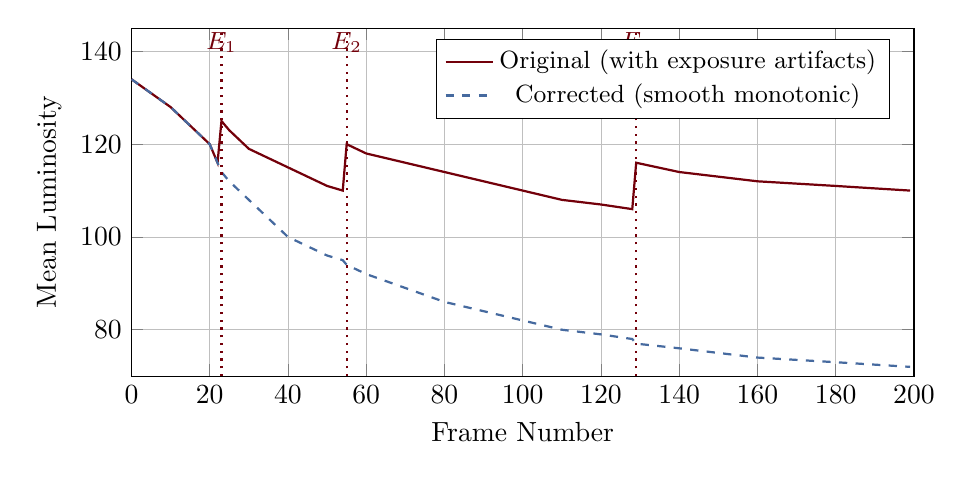
\begin{tikzpicture}
    \begin{axis}[
        width=0.95\textwidth,
        height=6cm,
        xlabel={Frame Number},
        ylabel={Mean Luminosity},
        xmin=0, xmax=200,
        ymin=70, ymax=145,
        grid=both,
        grid style={line width=0.1pt, draw=gray!30},
        major grid style={line width=0.2pt, draw=gray!50},
        legend pos=north east,
        legend style={font=\small},
    ]
    % Original data with jumps
    \addplot[color=garnet, thick, mark=none] coordinates {
        (0,134) (5,131) (10,128) (15,124) (20,120) (22,116) (23,125) (25,123) (30,119) (35,117) (40,115) (45,113) (50,111) (54,110) (55,120) (60,118) (70,116) (80,114) (90,112) (100,110) (110,108) (120,107) (128,106) (129,116) (140,114) (150,113) (160,112) (180,111) (199,110)
    };
    \addlegendentry{Original (with exposure artifacts)}

    % Corrected data - smooth monotonic decrease
    \addplot[color=atlantic, thick, mark=none, dashed] coordinates {
        (0,134) (5,131) (10,128) (15,124) (20,120) (22,116) (23,114) (25,112) (30,108) (35,104) (40,100) (45,98) (50,96) (54,95) (55,94) (60,92) (70,89) (80,86) (90,84) (100,82) (110,80) (120,79) (128,78) (129,77) (140,76) (150,75) (160,74) (180,73) (199,72)
    };
    \addlegendentry{Corrected (smooth monotonic)}

    % Mark exposure events
    \draw[garnet, thick, dotted] (axis cs:23,70) -- (axis cs:23,145);
    \draw[garnet, thick, dotted] (axis cs:55,70) -- (axis cs:55,145);
    \draw[garnet, thick, dotted] (axis cs:129,70) -- (axis cs:129,145);

    \node[font=\small, garnet] at (axis cs:23,142) {$E_1$};
    \node[font=\small, garnet] at (axis cs:55,142) {$E_2$};
    \node[font=\small, garnet] at (axis cs:129,142) {$E_3$};
    \end{axis}
\end{tikzpicture}
\caption{Luminosity profile during VARTM monitoring showing three auto-exposure compensation events ($E_1$ at frame 23, $E_2$ at frame 55, $E_3$ at frame 129). The original video (solid red) exhibits a characteristic sawtooth pattern where brightness suddenly increases despite continuous resin-induced darkening. Our corrected profile (dashed blue) produces smooth monotonically decreasing luminosity consistent with progressive resin coverage.}
\label{fig:luminosity_overview}
\end{figure*}

These exposure discontinuities pose significant challenges for computer vision algorithms used in flow-front detection and process monitoring. Threshold-based segmentation methods interpret sudden brightness changes as physical flow-front movement and produce false positive detections. Temporal differencing methods register large intensity changes at exposure boundaries unrelated to actual resin flow. Reference-based comparison methods become unreliable when the reference and current frames have different exposure levels. Machine learning approaches may fail to generalize when inference data contains exposure artifacts not present in training data.

The contribution of this paper is a comprehensive two-step correction methodology. The first step detects exposure compensation events through derivative analysis of luminosity signals extracted from stable image regions, then corrects brightness discontinuities using multiplicative scaling in CIELAB color space. The second step preserves original color relationships through frame-by-frame ratio normalization. The method requires no hardware modifications and operates automatically without manual parameter tuning.

\section{Background}
\label{sec:background}

\subsection{VARTM Process and Visual Monitoring}

In VARTM manufacturing, liquid thermoset resin is drawn through dry fiber reinforcement preforms using vacuum pressure differential. The resin flow-front propagates through the preform according to Darcy's law:

\begin{equation}
\vec{v} = -\frac{K}{\mu} \nabla P
\label{eq:darcy}
\end{equation}

where $\vec{v}$ is the superficial velocity, $K$ is the permeability tensor, $\mu$ is the resin viscosity, and $\nabla P$ is the pressure gradient. Visual monitoring enables tracking of the flow-front position $\mathbf{x}_f(t)$ over time for process validation and defect detection.

\subsection{Auto-Exposure Behavior}

Modern cameras employ automatic exposure control to maintain consistent image brightness. The exposure value is adjusted based on scene metering:

\begin{equation}
EV = \log_2\left(\frac{N^2}{t}\right) + \log_2\left(\frac{L_s}{K_m}\right)
\label{eq:exposure}
\end{equation}

where $N$ is the f-number, $t$ is the shutter time, $L_s$ is scene luminance, and $K_m$ is a metering constant. Each discrete adjustment event produces a multiplicative brightness change:

\begin{equation}
I'(x,y) = \alpha \cdot I(x,y) + \beta
\label{eq:exposure_change}
\end{equation}

\begin{figure*}[t]
\centering
\begin{subfigure}[b]{0.49\textwidth}
    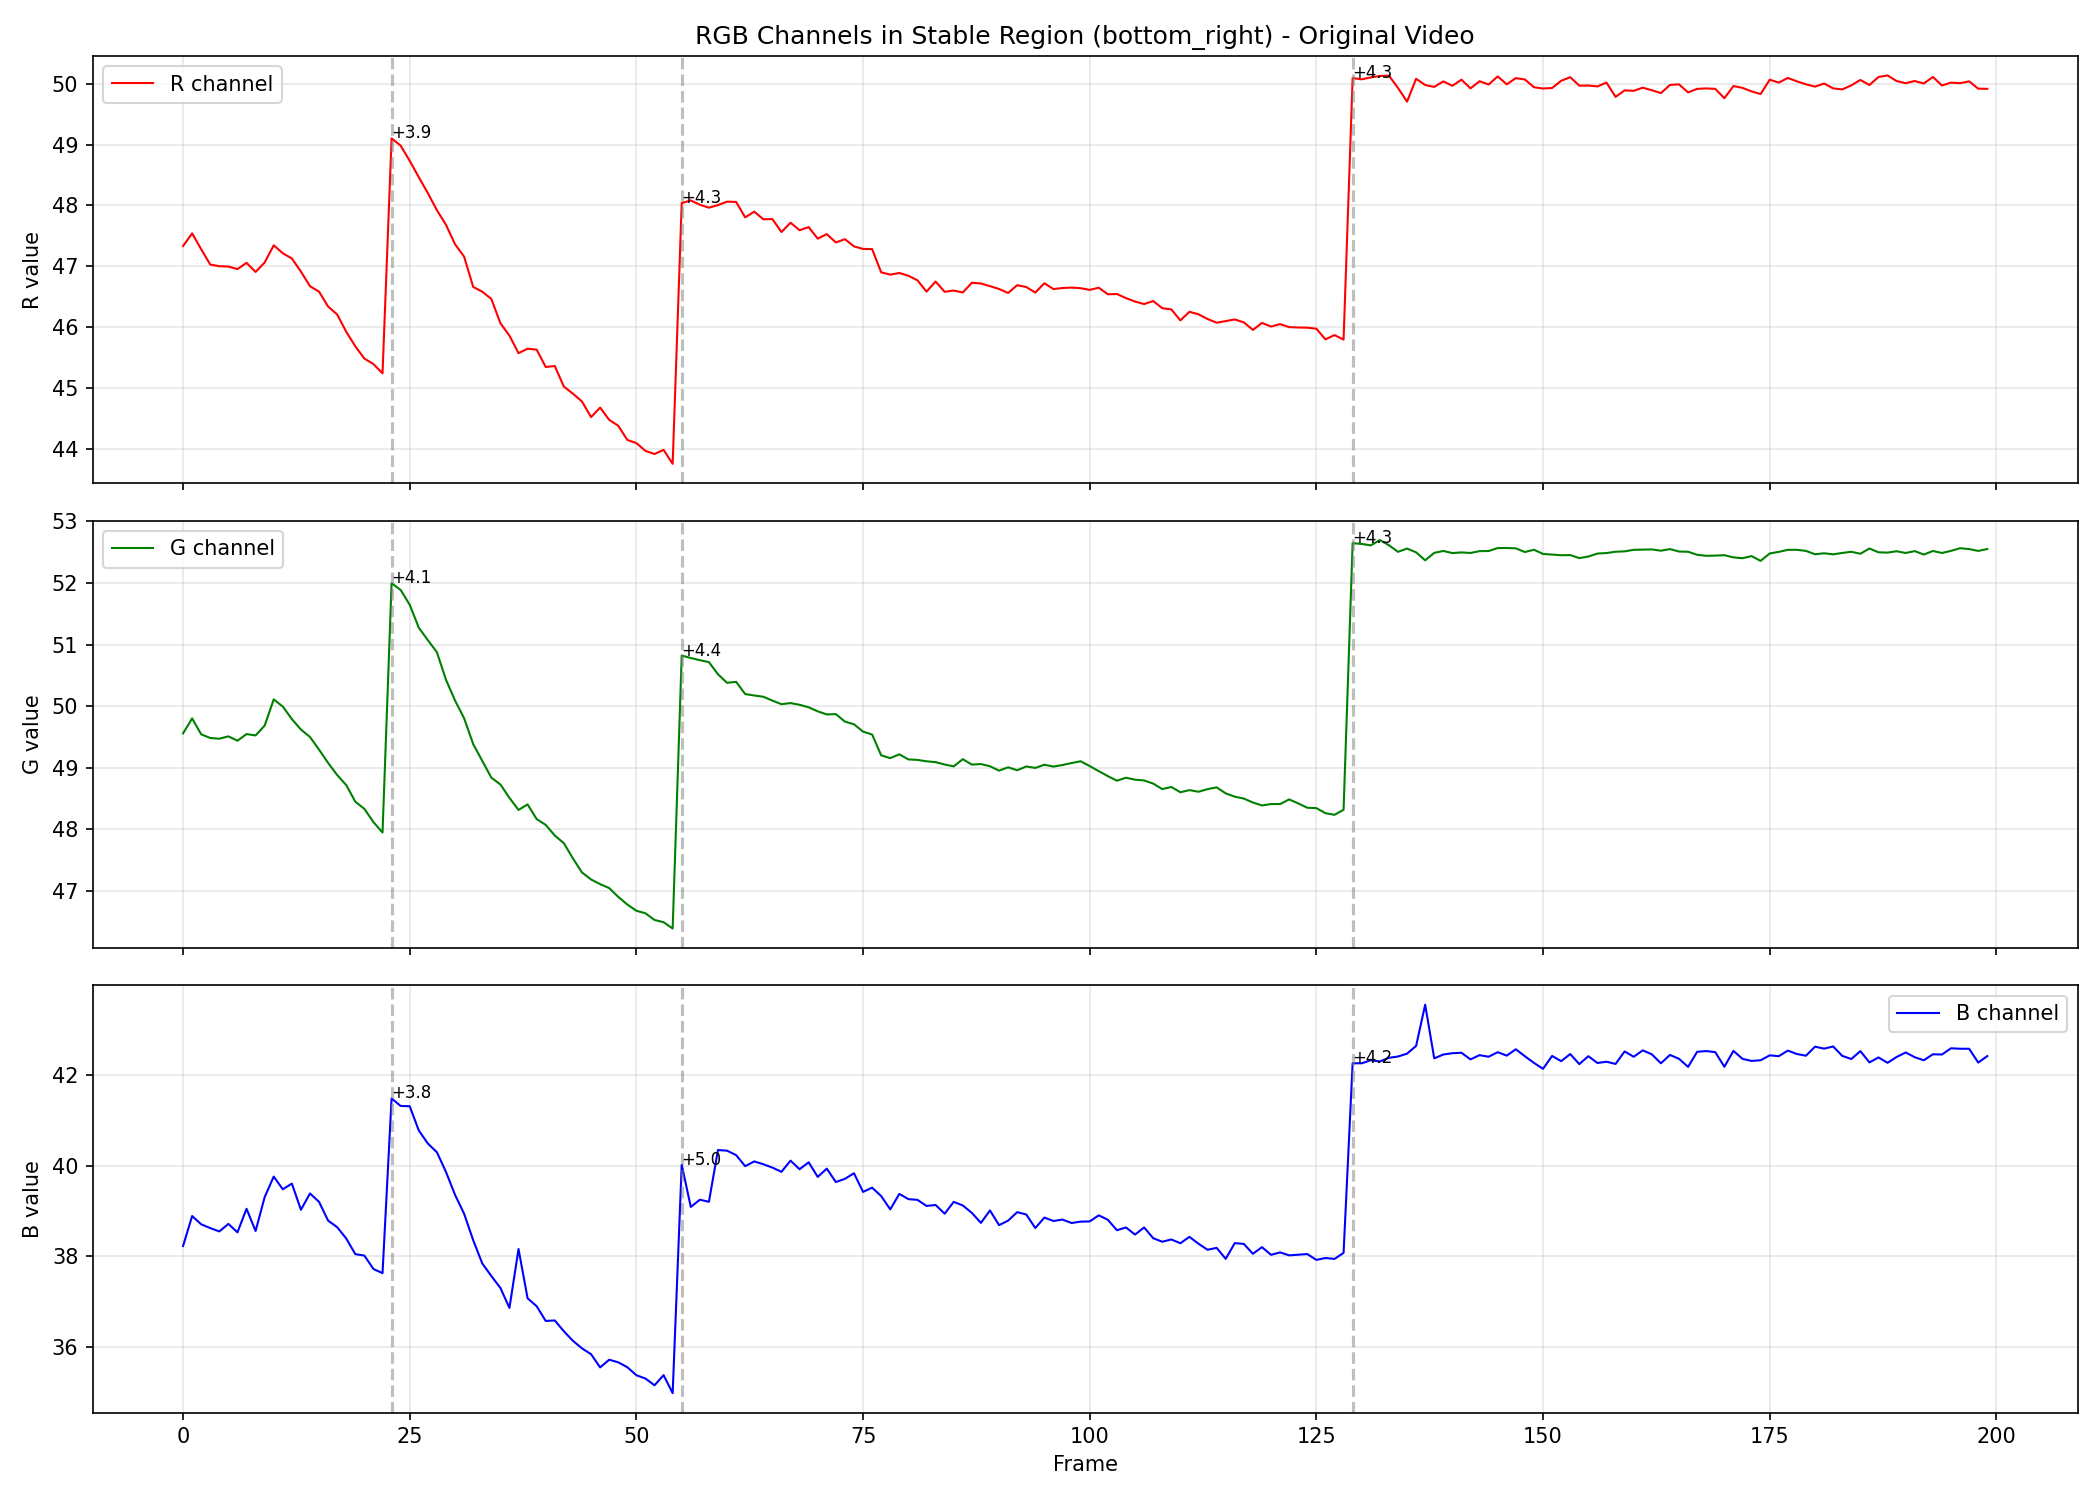
\includegraphics[width=\textwidth]{figures/rgb_analysis.png}
    \caption{RGB channel analysis showing differential response}
\end{subfigure}
\hfill
\begin{subfigure}[b]{0.49\textwidth}
    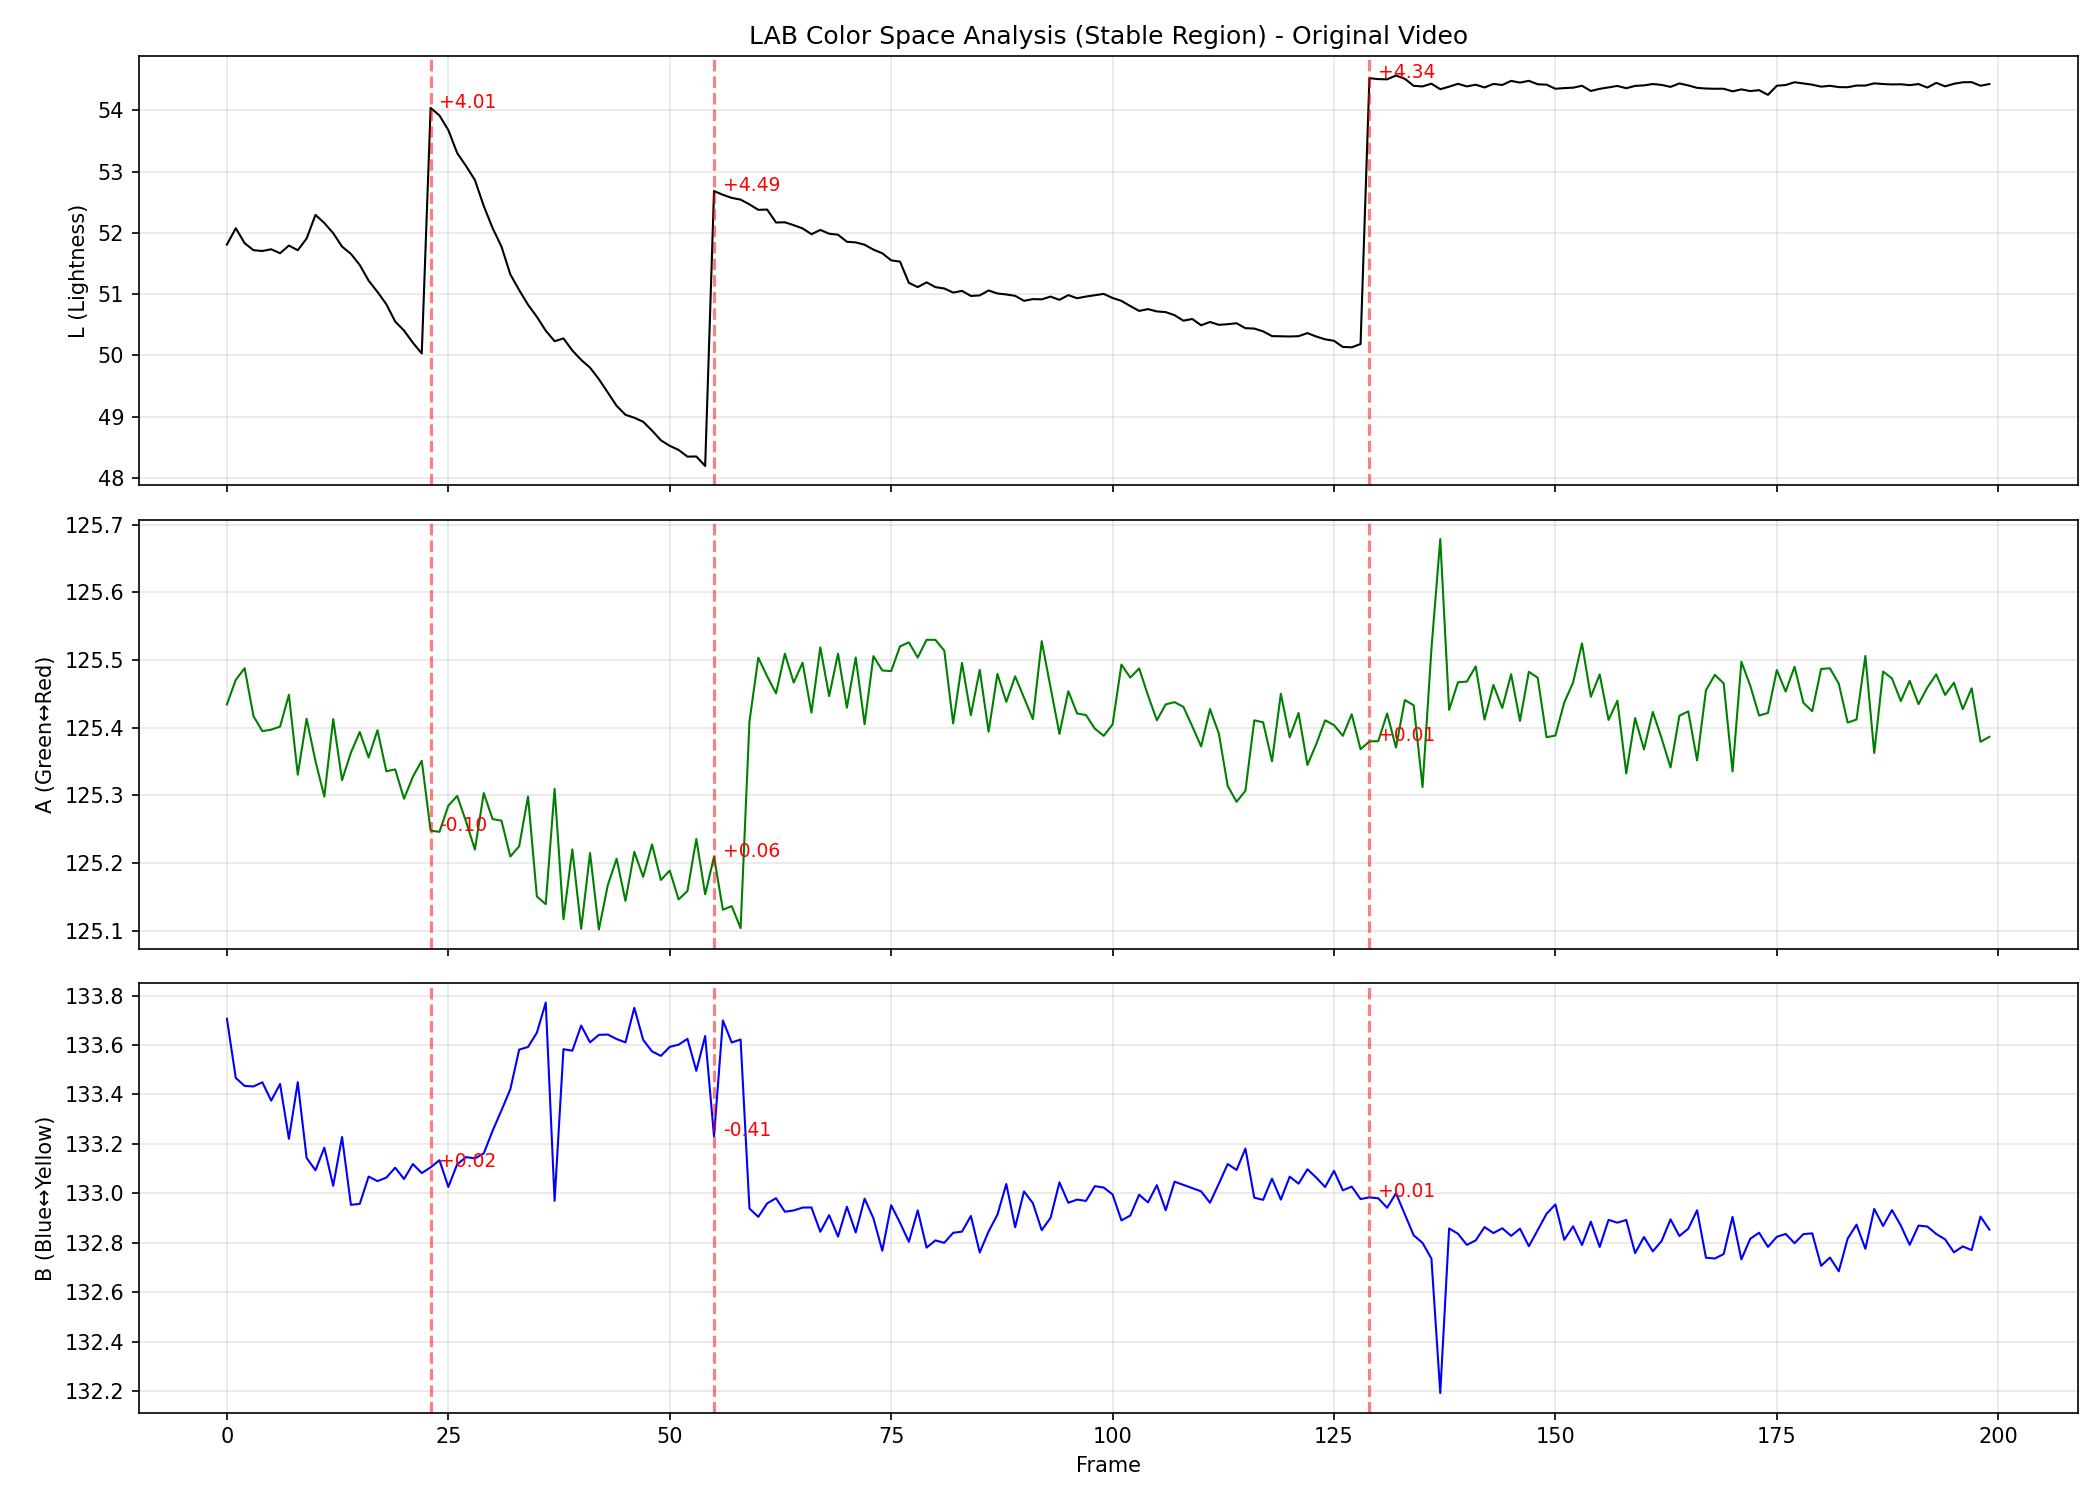
\includegraphics[width=\textwidth]{figures/lab_analysis.png}
    \caption{LAB analysis showing $L^*$ jumps with stable $a^*$, $b^*$}
\end{subfigure}
\caption{Color space analysis of exposure events in the stable reference region. (a) RGB channels all exhibit jumps but with different magnitudes---the blue channel increases more (+5.0) at frame 55 than red (+4.3) or green (+4.4). (b) In LAB space, only the $L^*$ lightness channel shows significant change (+4.0 to +4.5 units); chromatic channels $a^*$ and $b^*$ remain essentially constant, validating $L^*$-only correction.}
\label{fig:color_analysis}
\end{figure*}

\begin{figure*}[t]
\centering
\begin{subfigure}[b]{0.49\textwidth}
    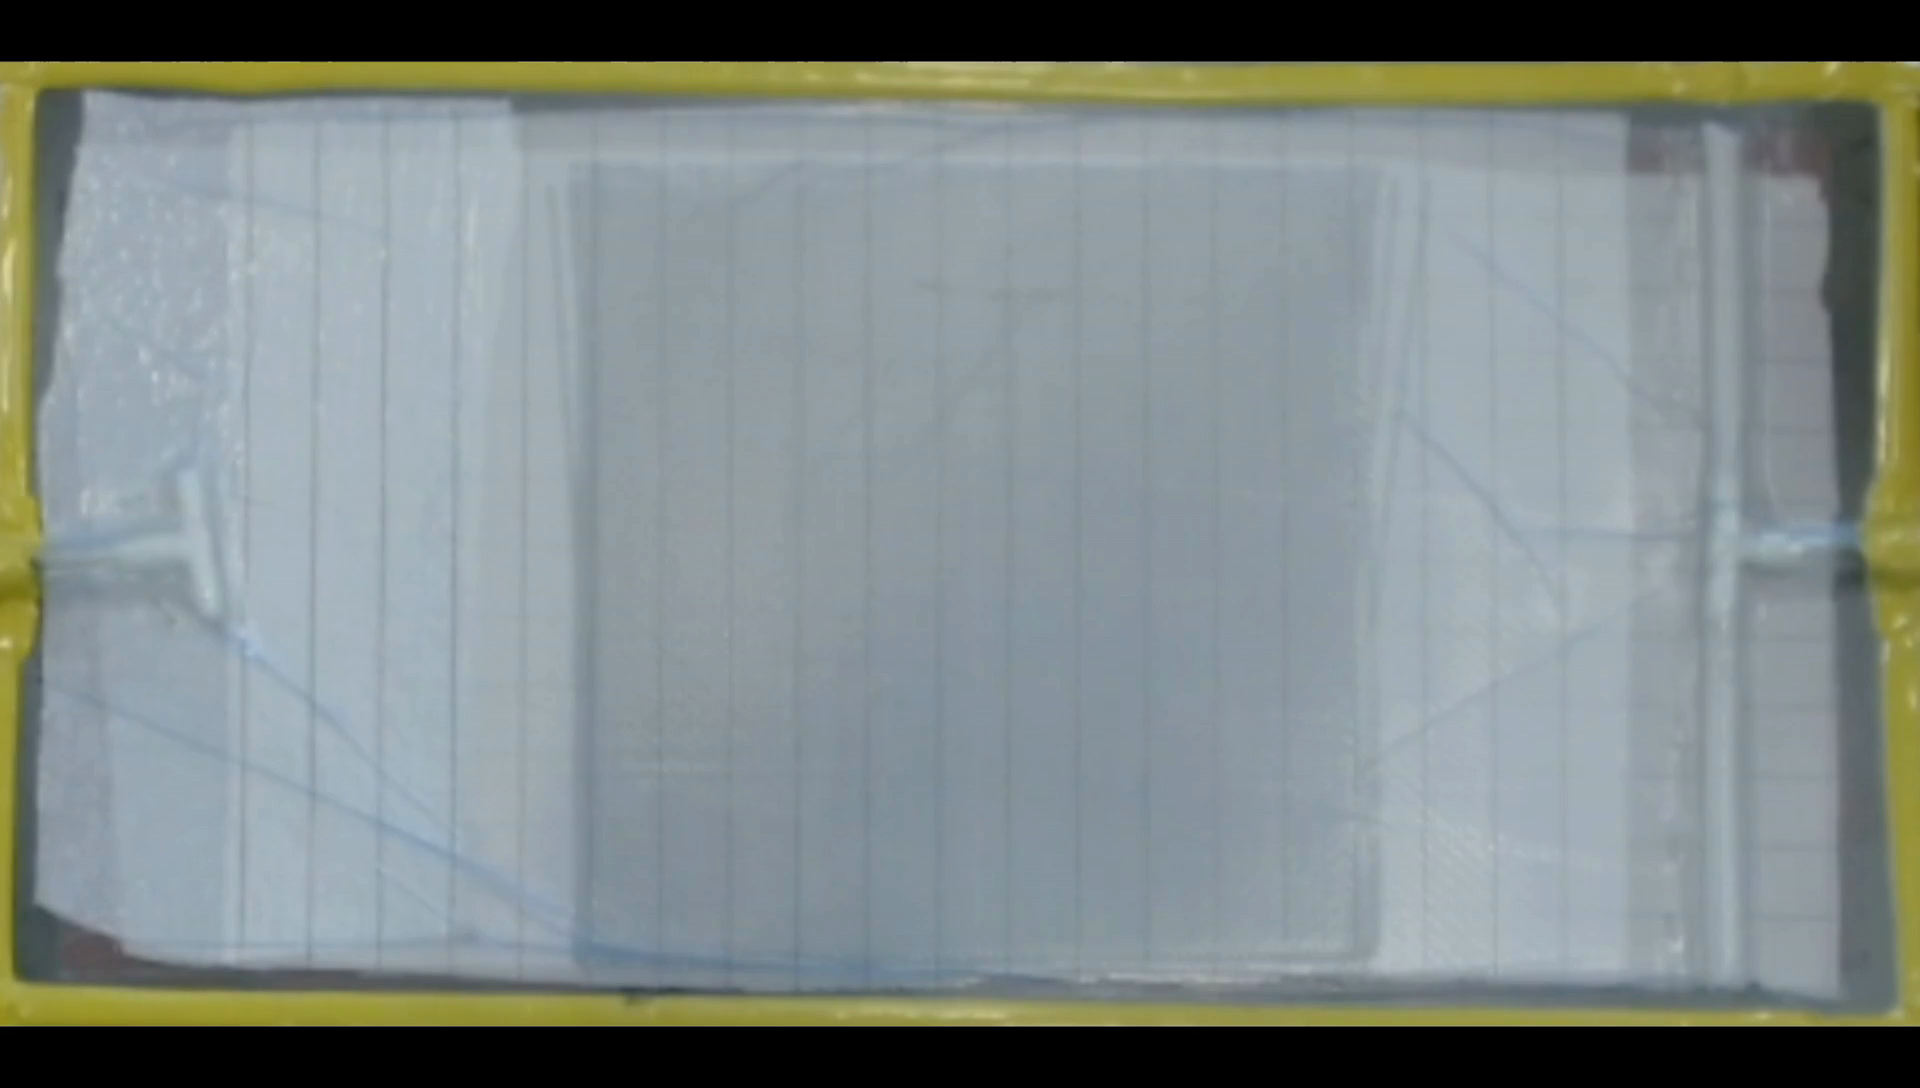
\includegraphics[width=\textwidth]{figures/original_frame_000.png}
    \caption{Original frame 0 (dry preform)}
\end{subfigure}
\hfill
\begin{subfigure}[b]{0.49\textwidth}
    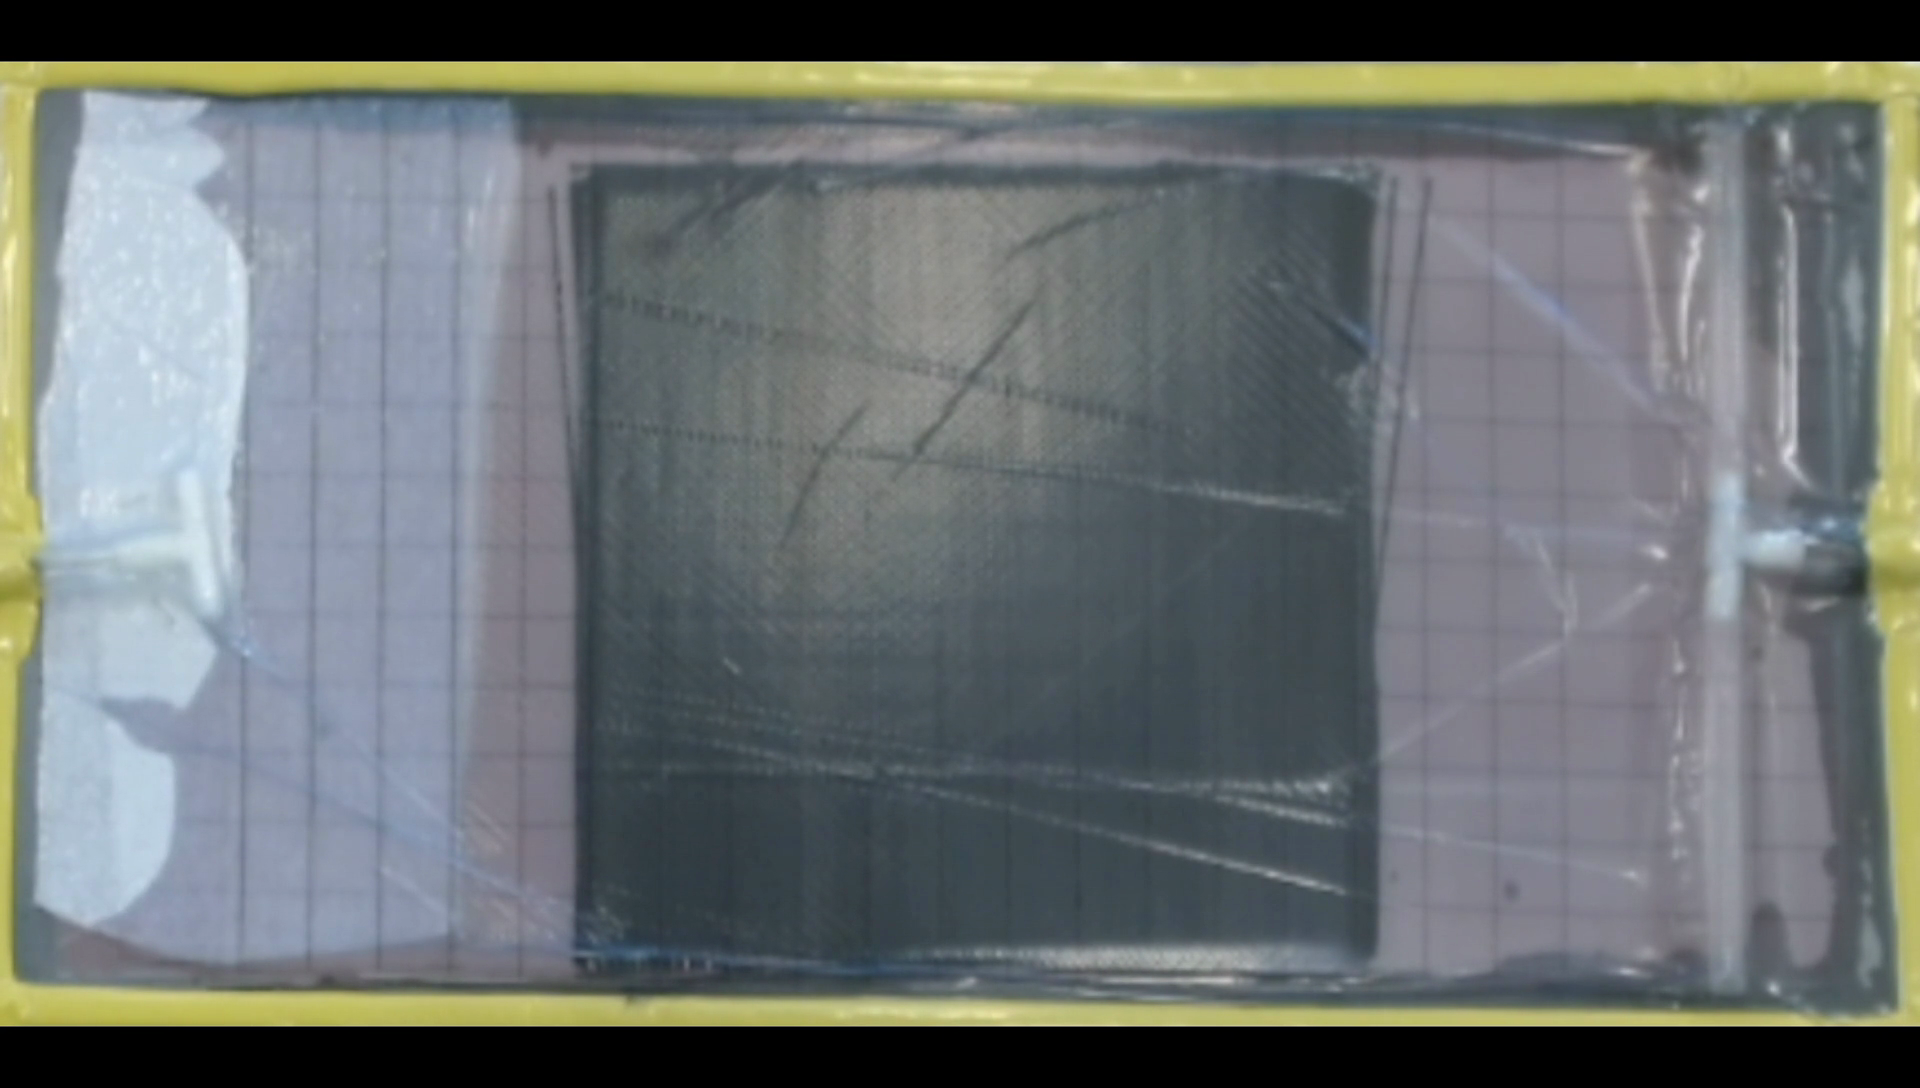
\includegraphics[width=\textwidth]{figures/original_frame_199.png}
    \caption{Original frame 199 (near complete infusion)}
\end{subfigure}
\caption{VARTM infusion video start and end frames. Frame 0 shows the dry fiber preform before resin introduction, with bright appearance due to light scattering from dry fibers. Frame 199 shows near-complete resin coverage, with significant darkening as resin absorption reduces light scattering. The mean luminosity decreases from 134 to 110 over this 60-second infusion sequence.}
\label{fig:start_end}
\end{figure*}

\subsection{Color Space Considerations}

The CIELAB color space provides a perceptually-uniform representation where lightness $L^*$ is separated from chromatic dimensions $a^*$ (green-red) and $b^*$ (blue-yellow):

\begin{align}
L^* &= 116 f(Y/Y_n) - 16 \\
a^* &= 500 [f(X/X_n) - f(Y/Y_n)] \\
b^* &= 200 [f(Y/Y_n) - f(Z/Z_n)]
\end{align}

Our empirical analysis reveals that exposure compensation primarily affects $L^*$ while leaving $a^*$ and $b^*$ relatively unchanged, motivating our LAB-based correction approach.

\section{Methodology}
\label{sec:methodology}

Our correction pipeline consists of four stages: stable region identification, exposure event detection, LAB-space brightness correction, and color ratio normalization. Figure~\ref{fig:pipeline} illustrates the workflow.

\begin{figure}[t]
\centering
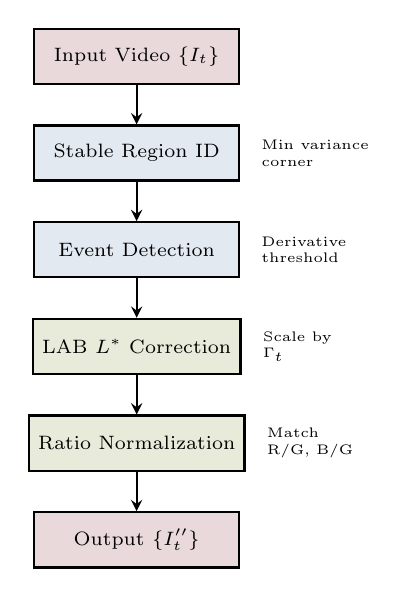
\begin{tikzpicture}[
    node distance=0.5cm,
    box/.style={rectangle, draw=uofscblack, thick, minimum width=2.6cm, minimum height=0.7cm, align=center, font=\scriptsize},
    arrow/.style={->, thick, >=stealth}
]
    \node[box, fill=garnet!15] (input) {Input Video $\{I_t\}$};
    \node[box, fill=atlantic!15, below=of input] (roi) {Stable Region ID};
    \node[box, fill=atlantic!15, below=of roi] (detect) {Event Detection};
    \node[box, fill=horseshoe!15, below=of detect] (lab) {LAB $L^*$ Correction};
    \node[box, fill=horseshoe!15, below=of lab] (color) {Ratio Normalization};
    \node[box, fill=garnet!15, below=of color] (output) {Output $\{I''_t\}$};

    \draw[arrow] (input) -- (roi);
    \draw[arrow] (roi) -- (detect);
    \draw[arrow] (detect) -- (lab);
    \draw[arrow] (lab) -- (color);
    \draw[arrow] (color) -- (output);

    \node[right=0.15cm of roi, font=\tiny, align=left] {Min variance\\corner};
    \node[right=0.15cm of detect, font=\tiny, align=left] {Derivative\\threshold};
    \node[right=0.15cm of lab, font=\tiny, align=left] {Scale by\\$\Gamma_t$};
    \node[right=0.15cm of color, font=\tiny, align=left] {Match\\R/G, B/G};
\end{tikzpicture}
\caption{Processing pipeline for two-step exposure correction.}
\label{fig:pipeline}
\end{figure}

\subsection{Stable Region Identification}

To isolate camera behavior from physical resin flow, we identify stable image regions outside the infusion zone. For each candidate region $\Omega_k$, we compute temporal variance:

\begin{equation}
\sigma^2_k = \text{Var}\left[\frac{1}{|\Omega_k|}\sum_{(x,y)\in\Omega_k} I_t(x,y)\right]_{t=0}^{T-1}
\label{eq:region_variance}
\end{equation}

The region with minimum variance is selected: $\Omega^* = \arg\min_k \sigma^2_k$. Table~\ref{tab:region_variance} shows that the bottom-right corner exhibited lowest variance in our experiment.

\begin{table}[t]
\centering
\caption{Temporal variance for candidate stable regions.}
\label{tab:region_variance}
\begin{tabular}{lcc}
\toprule
\textbf{Region} & \textbf{Variance $\sigma^2$} & \textbf{Selected} \\
\midrule
Top-left corner & 2.87 & -- \\
Top-right corner & 3.42 & -- \\
Bottom-left corner & 1.95 & -- \\
Bottom-right corner & 0.30 & $\checkmark$ \\
Center region & 5.53 & -- \\
\bottomrule
\end{tabular}
\end{table}

\subsection{Exposure Event Detection}

Within the stable region, exposure events manifest as positive discontinuities. The frame-to-frame derivative is:

\begin{equation}
\Delta L_t = L_{t+1} - L_t
\label{eq:derivative}
\end{equation}

Events are detected where the smoothed derivative exceeds a threshold:

\begin{equation}
\mathcal{E} = \{t : \tilde{\Delta L}_t > \mu_{\Delta L} + \tau \cdot \sigma_{\Delta L}\}
\label{eq:event_detection}
\end{equation}

Adjacent detections are consolidated, selecting the frame with largest jump as the event location.

\begin{figure}[t]
\centering
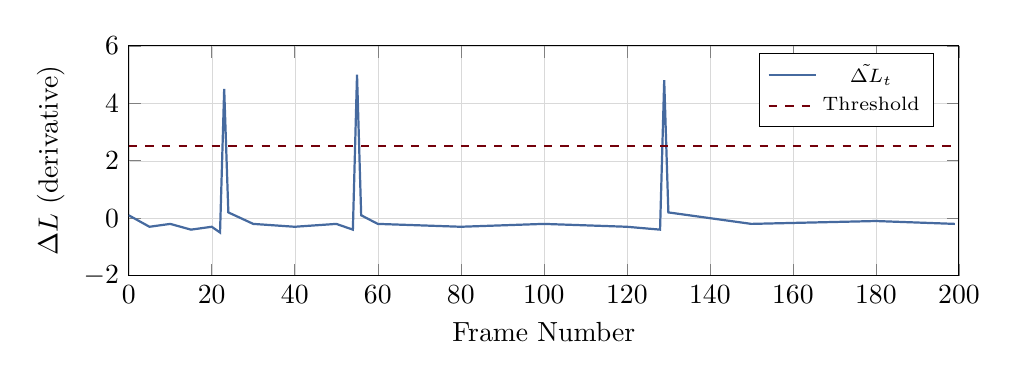
\begin{tikzpicture}
    \begin{axis}[
        width=\columnwidth,
        height=4.5cm,
        xlabel={Frame Number},
        ylabel={$\Delta L$ (derivative)},
        xmin=0, xmax=200,
        ymin=-2, ymax=6,
        grid=both,
        grid style={line width=0.1pt, draw=gray!30},
        legend pos=north east,
        legend style={font=\scriptsize},
    ]
    \addplot[color=atlantic, thick, mark=none] coordinates {
        (0,0.1) (5,-0.3) (10,-0.2) (15,-0.4) (20,-0.3) (22,-0.5) (23,4.5) (24,0.2) (30,-0.2) (40,-0.3) (50,-0.2) (54,-0.4) (55,5.0) (56,0.1) (60,-0.2) (80,-0.3) (100,-0.2) (120,-0.3) (128,-0.4) (129,4.8) (130,0.2) (150,-0.2) (180,-0.1) (199,-0.2)
    };
    \addlegendentry{$\tilde{\Delta L}_t$}

    \addplot[color=garnet, thick, dashed, mark=none] coordinates {
        (0,2.5) (199,2.5)
    };
    \addlegendentry{Threshold}
    \end{axis}
\end{tikzpicture}
\caption{Derivative-based detection showing peaks at frames 23, 55, and 129 exceeding the threshold, indicating exposure events.}
\label{fig:derivative_detection}
\end{figure}

\subsection{LAB L*-Channel Correction}

For each detected event $t_e$, we compute the correction factor:

\begin{equation}
\gamma_{t_e} = \frac{L^*_{t_e - 1}}{L^*_{t_e}}
\label{eq:correction_factor}
\end{equation}

Factors are applied cumulatively: $\Gamma_t = \prod_{t_e \leq t} \gamma_{t_e}$

The corrected lightness channel is: $L'^*(x,y,t) = \Gamma_t \cdot L^*(x,y,t)$

\subsection{Color Ratio Normalization}

To ensure perfect color fidelity, we normalize RGB ratios to match the original:

\begin{align}
\alpha^R_t &= \frac{R_t / G_t}{R'_t / G'_t}, \quad
\alpha^B_t = \frac{B_t / G_t}{B'_t / G'_t}
\end{align}

Final correction: $R'' = \alpha^R_t R'$, $G'' = G'$, $B'' = \alpha^B_t B'$

\begin{algorithm}[t]
\caption{Two-Step Exposure Correction}
\label{alg:complete}
\begin{algorithmic}[1]
\REQUIRE Video $\{I_t\}$, threshold $\tau$
\ENSURE Corrected video $\{I''_t\}$
\STATE Find stable region $\Omega^*$ with min temporal variance
\STATE Compute $L_t$ = mean $L^*$ in $\Omega^*$ for all frames
\STATE Detect events $\mathcal{E}$ where $\Delta L > \mu + \tau\sigma$
\FOR{each event $t_e \in \mathcal{E}$}
    \STATE $\gamma_{t_e} \leftarrow L^*_{t_e-1} / L^*_{t_e}$
\ENDFOR
\FOR{$t = 0$ to $T-1$}
    \STATE $\Gamma_t \leftarrow \prod_{t_e \leq t} \gamma_{t_e}$
    \STATE Scale $L^*$ by $\Gamma_t$ $\rightarrow I'_t$
    \STATE Normalize R/G, B/G ratios $\rightarrow I''_t$
\ENDFOR
\RETURN $\{I''_t\}$
\end{algorithmic}
\end{algorithm}

\section{Experimental Results}
\label{sec:results}

\subsection{Dataset and Setup}

We evaluated our method on a VARTM infusion video at $1920 \times 1088$ resolution, 3.33 fps, totaling 200 frames over 60 seconds. The camera's auto-exposure was enabled, resulting in three exposure events.

\subsection{Detection Results}

Table~\ref{tab:detection_results} shows the detected events and correction factors.

\begin{table}[t]
\centering
\caption{Detected exposure events and correction factors.}
\label{tab:detection_results}
\begin{tabular}{ccccc}
\toprule
\textbf{Event} & \textbf{Frame} & \textbf{$L^*$ Jump} & \textbf{$\gamma$} & \textbf{$\Gamma$} \\
\midrule
$E_1$ & 23 & $50.0 \rightarrow 54.0$ & 0.926 & 0.926 \\
$E_2$ & 55 & $48.2 \rightarrow 52.7$ & 0.915 & 0.847 \\
$E_3$ & 129 & $50.2 \rightarrow 54.5$ & 0.921 & 0.780 \\
\bottomrule
\end{tabular}
\end{table}

\subsection{Visual Comparison at Event Boundaries}

Figures~\ref{fig:visual_comparison_e1}, \ref{fig:visual_comparison_e2}, and \ref{fig:visual_comparison_e3} show frame comparisons at each exposure event boundary. In each case, the original video exhibits visible brightness discontinuity between adjacent frames despite minimal physical change in resin coverage. The corrected video maintains smooth temporal consistency aligned with the natural resin flow progression.

\begin{figure*}[t]
\centering
\begin{subfigure}[b]{0.32\textwidth}
    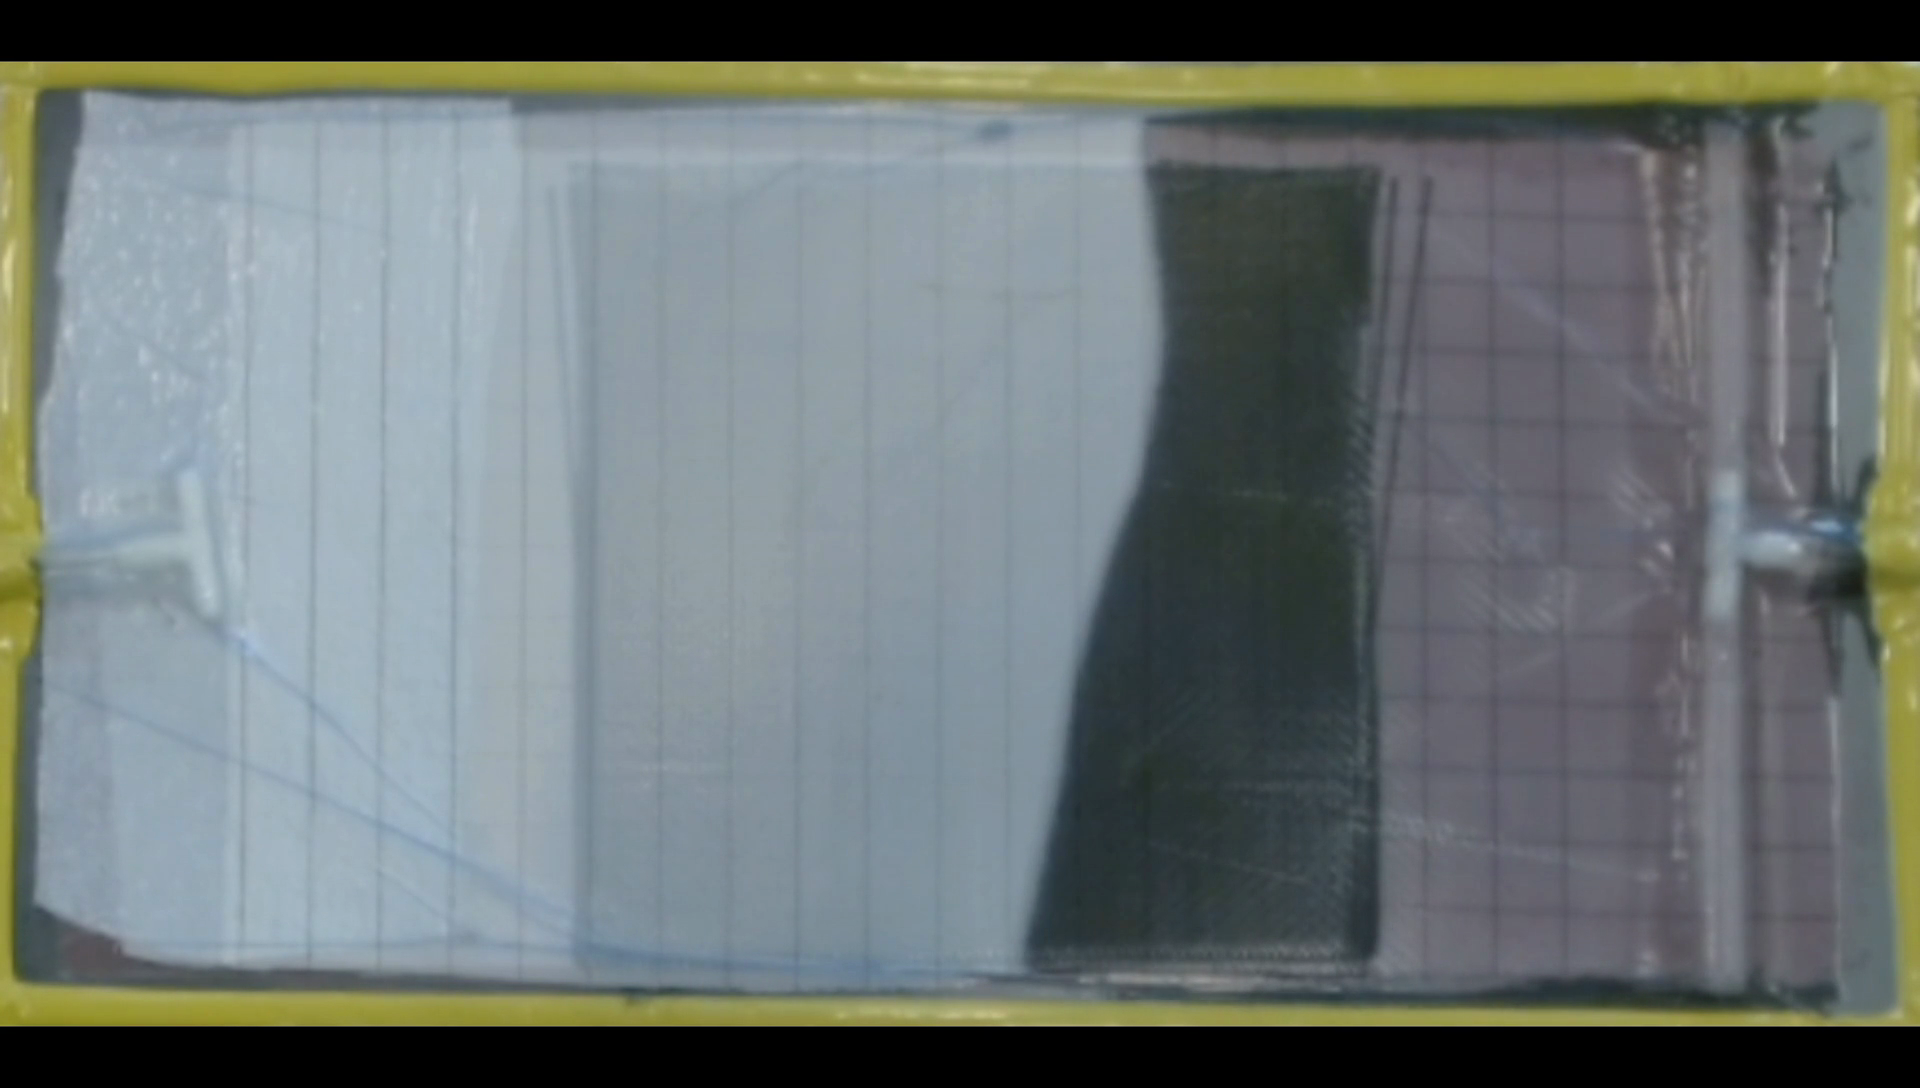
\includegraphics[width=\textwidth]{figures/original_frame_022.png}
    \caption{Original, frame 22}
\end{subfigure}
\hfill
\begin{subfigure}[b]{0.32\textwidth}
    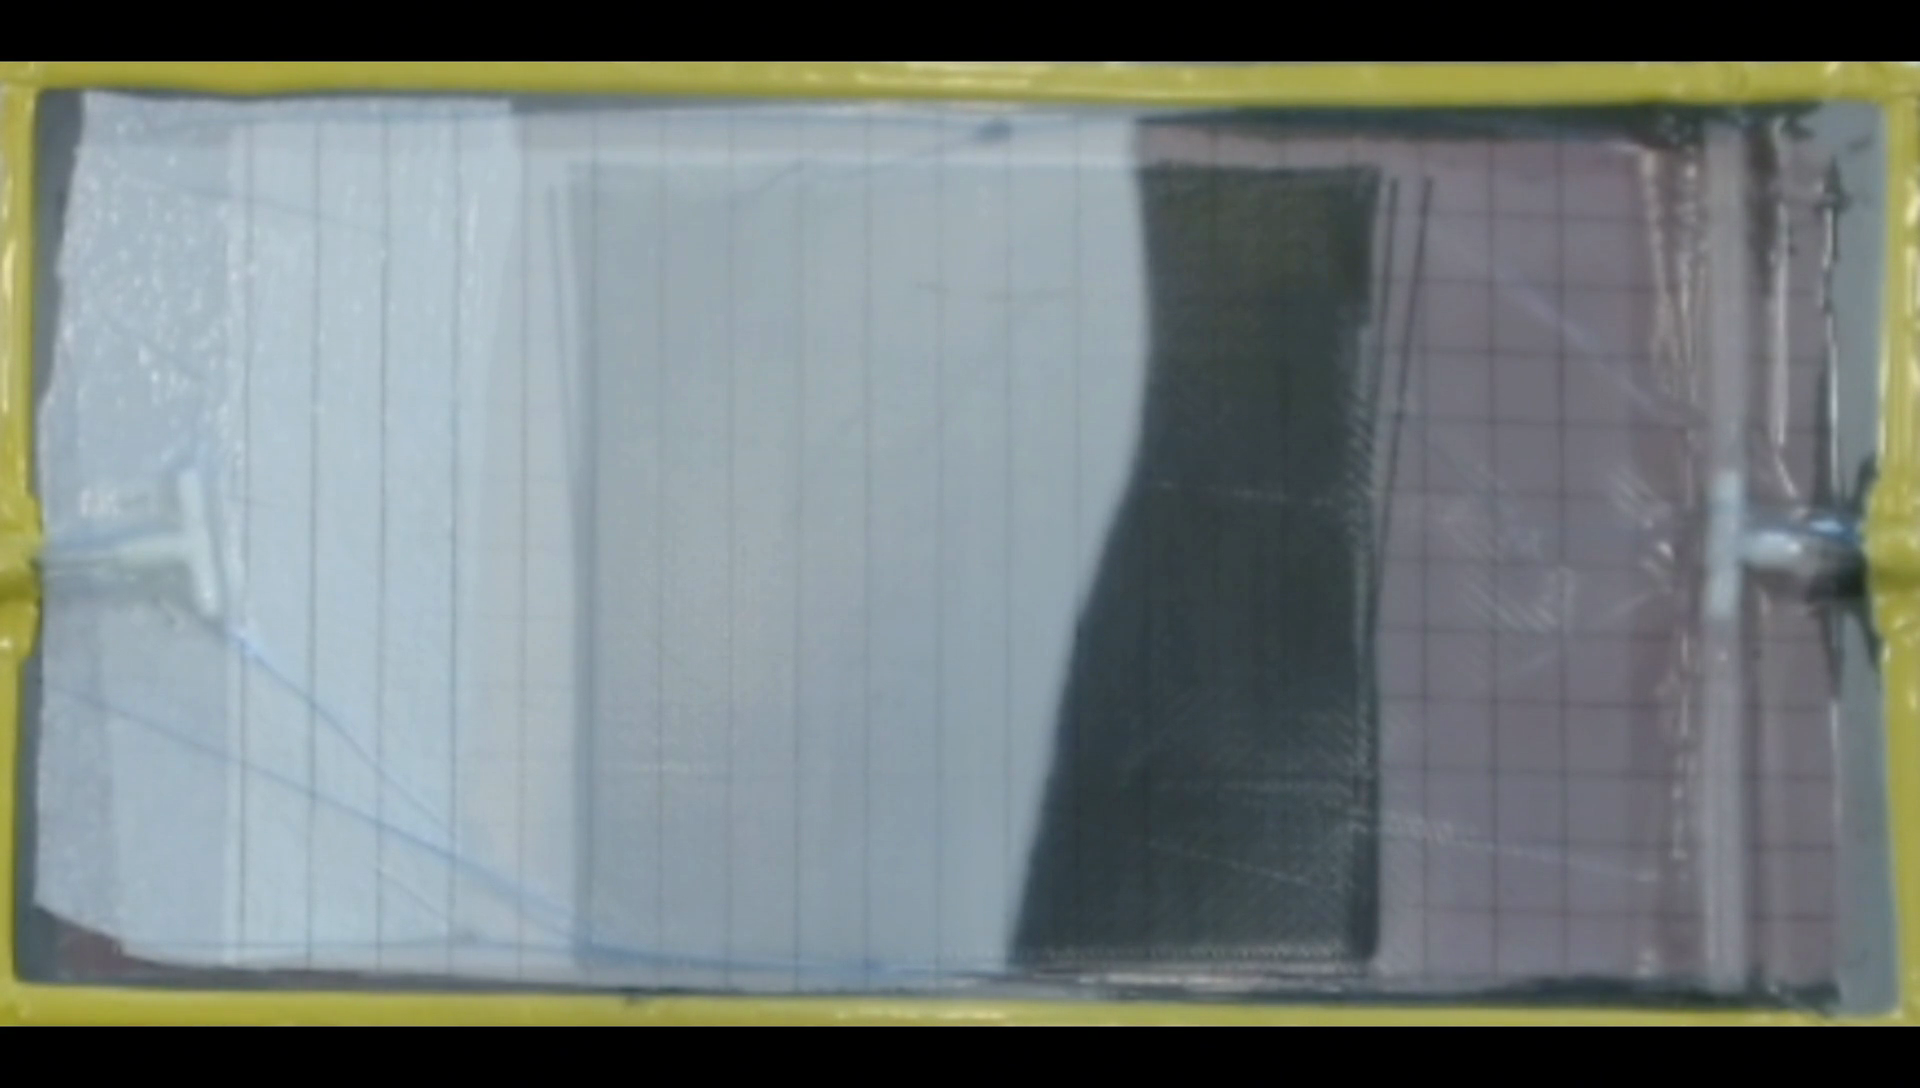
\includegraphics[width=\textwidth]{figures/original_frame_023.png}
    \caption{Original, frame 23 (event)}
\end{subfigure}
\hfill
\begin{subfigure}[b]{0.32\textwidth}
    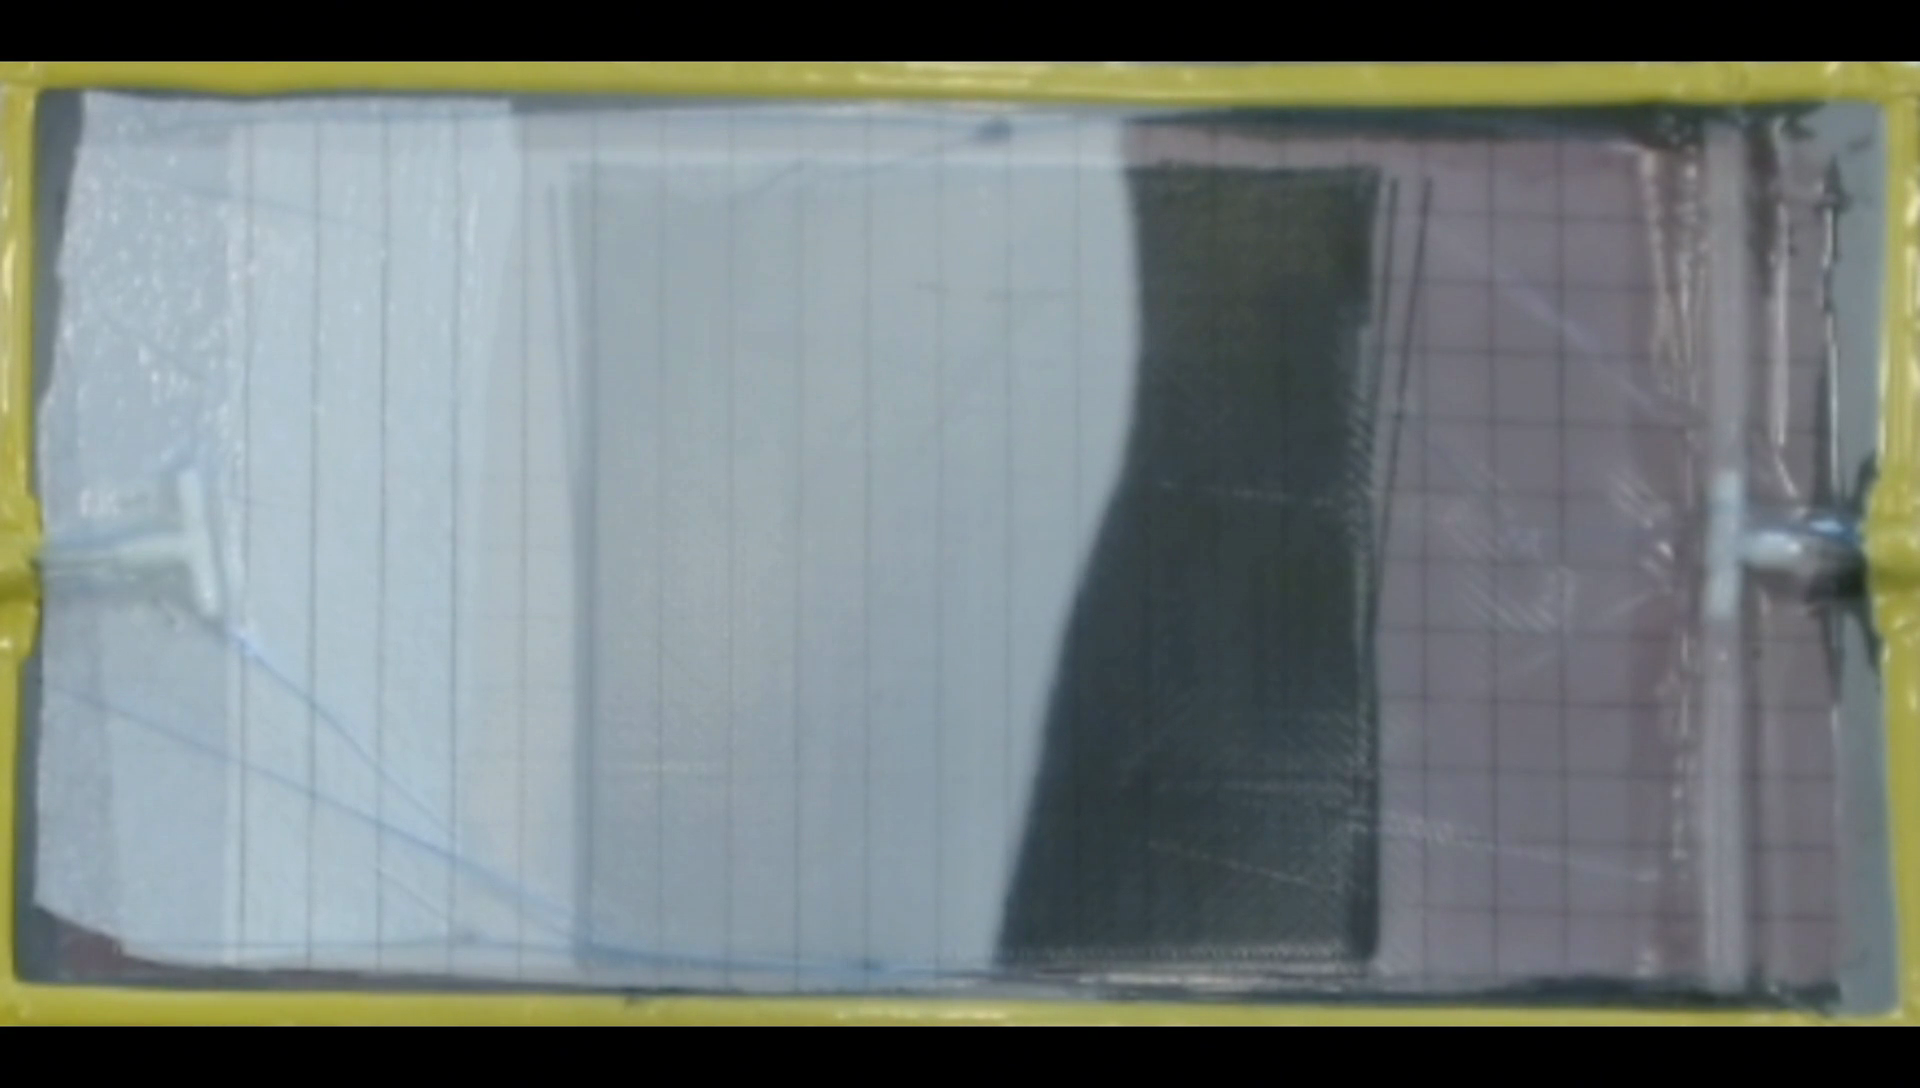
\includegraphics[width=\textwidth]{figures/original_frame_024.png}
    \caption{Original, frame 24}
\end{subfigure}
\\[0.5em]
\begin{subfigure}[b]{0.32\textwidth}
    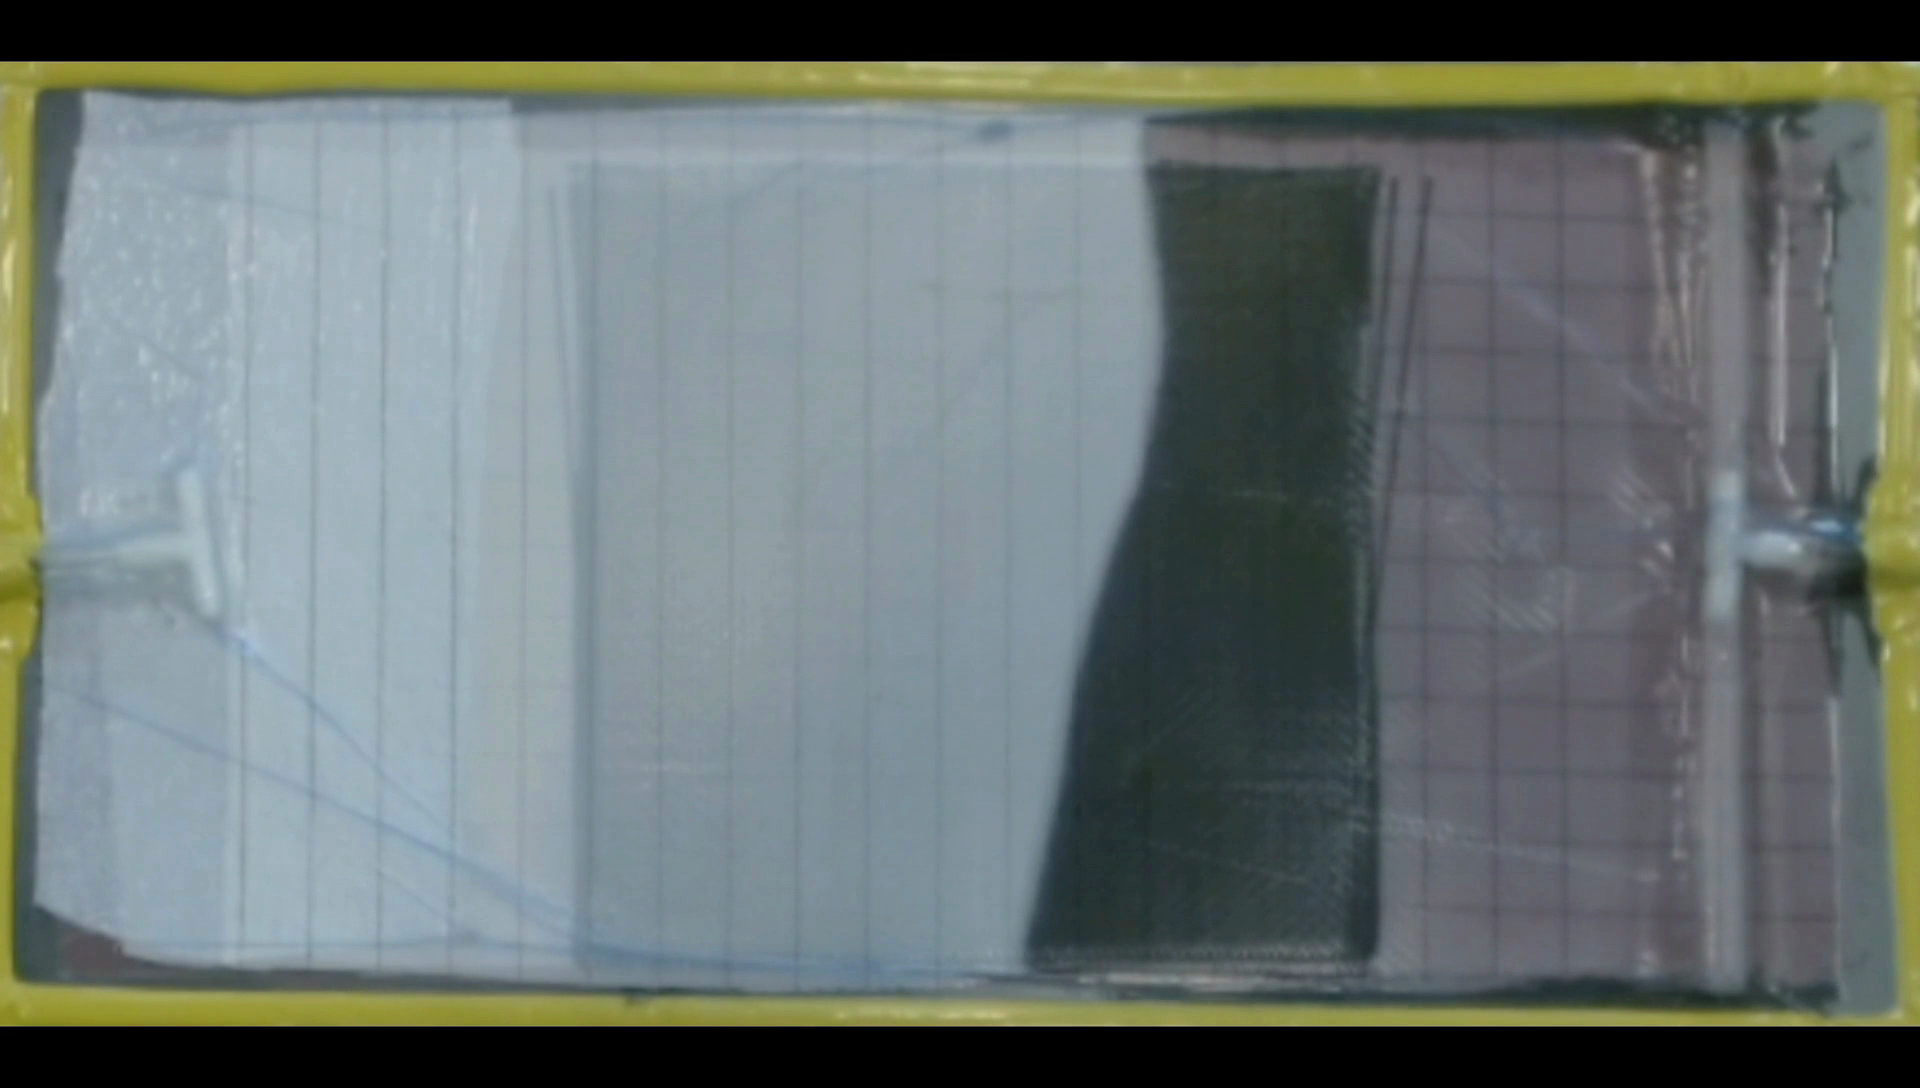
\includegraphics[width=\textwidth]{figures/corrected_frame_022.png}
    \caption{Corrected, frame 22}
\end{subfigure}
\hfill
\begin{subfigure}[b]{0.32\textwidth}
    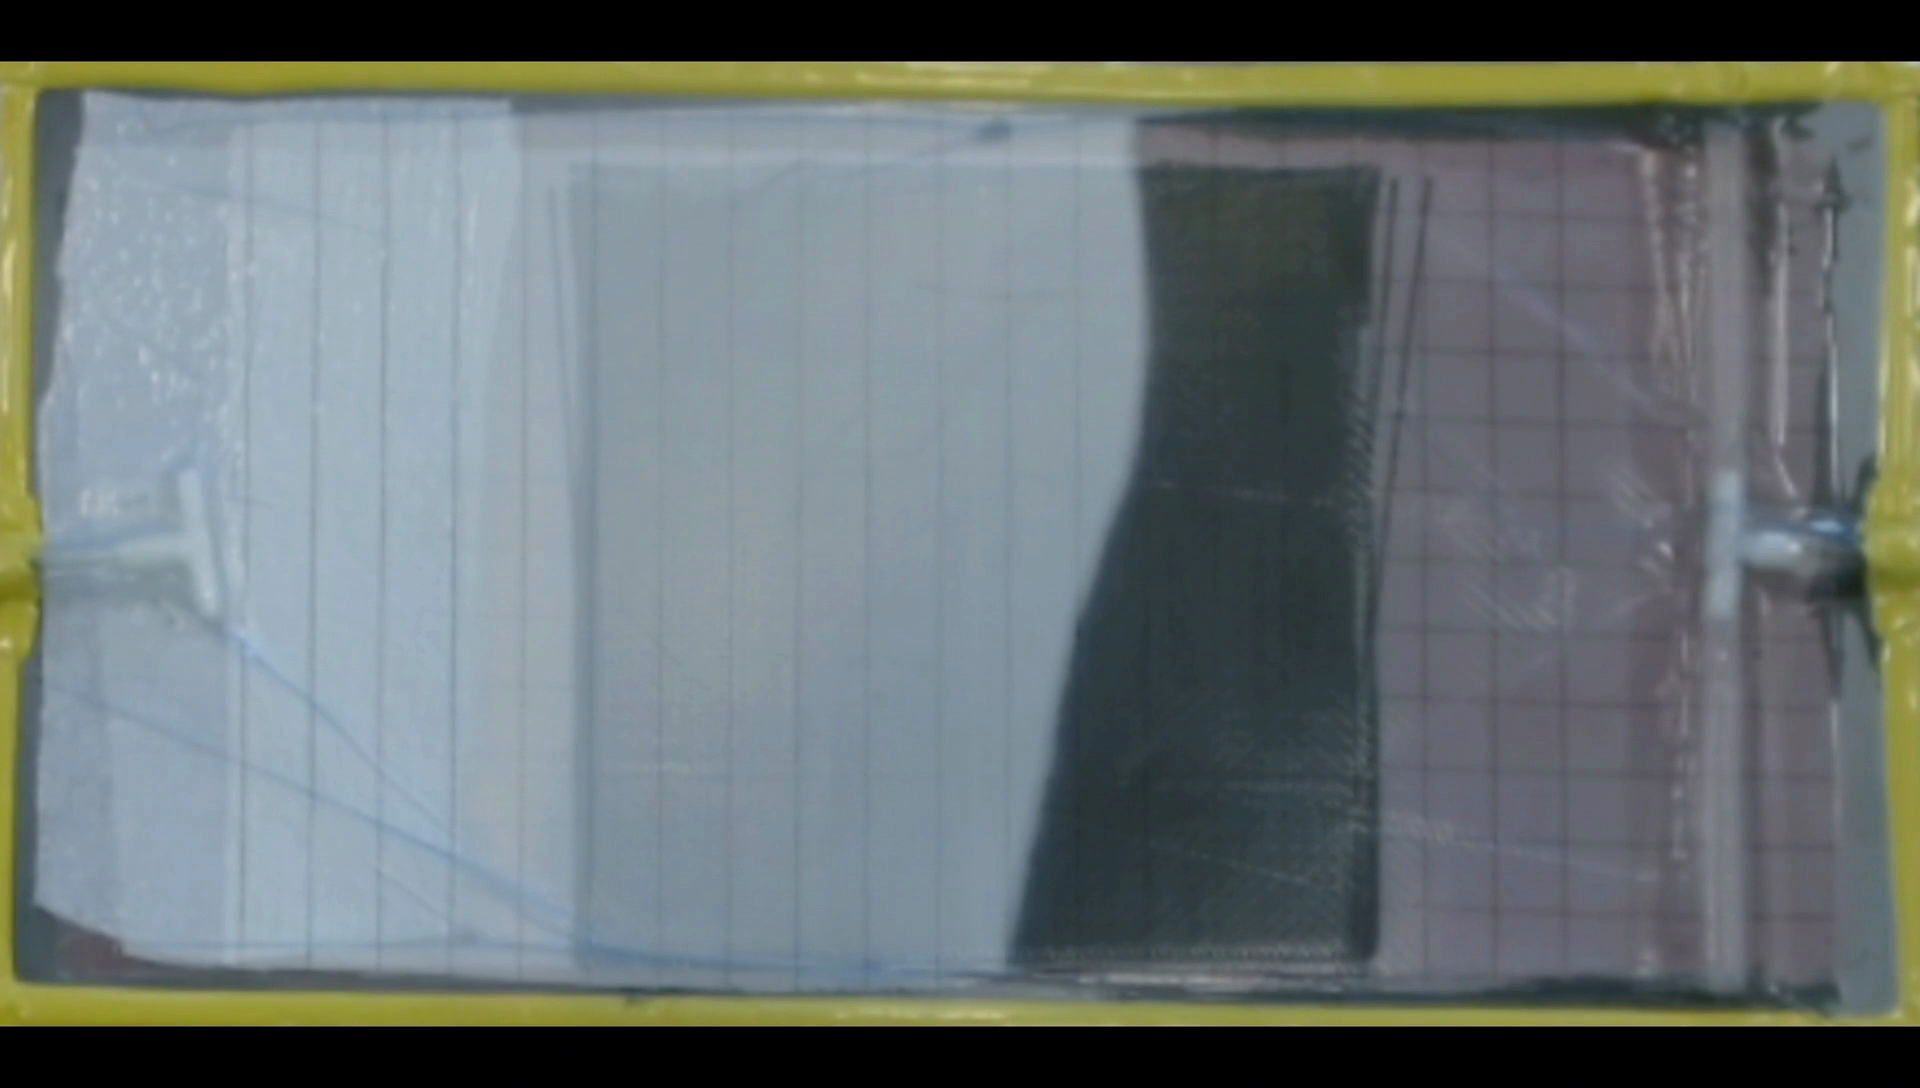
\includegraphics[width=\textwidth]{figures/corrected_frame_023.png}
    \caption{Corrected, frame 23}
\end{subfigure}
\hfill
\begin{subfigure}[b]{0.32\textwidth}
    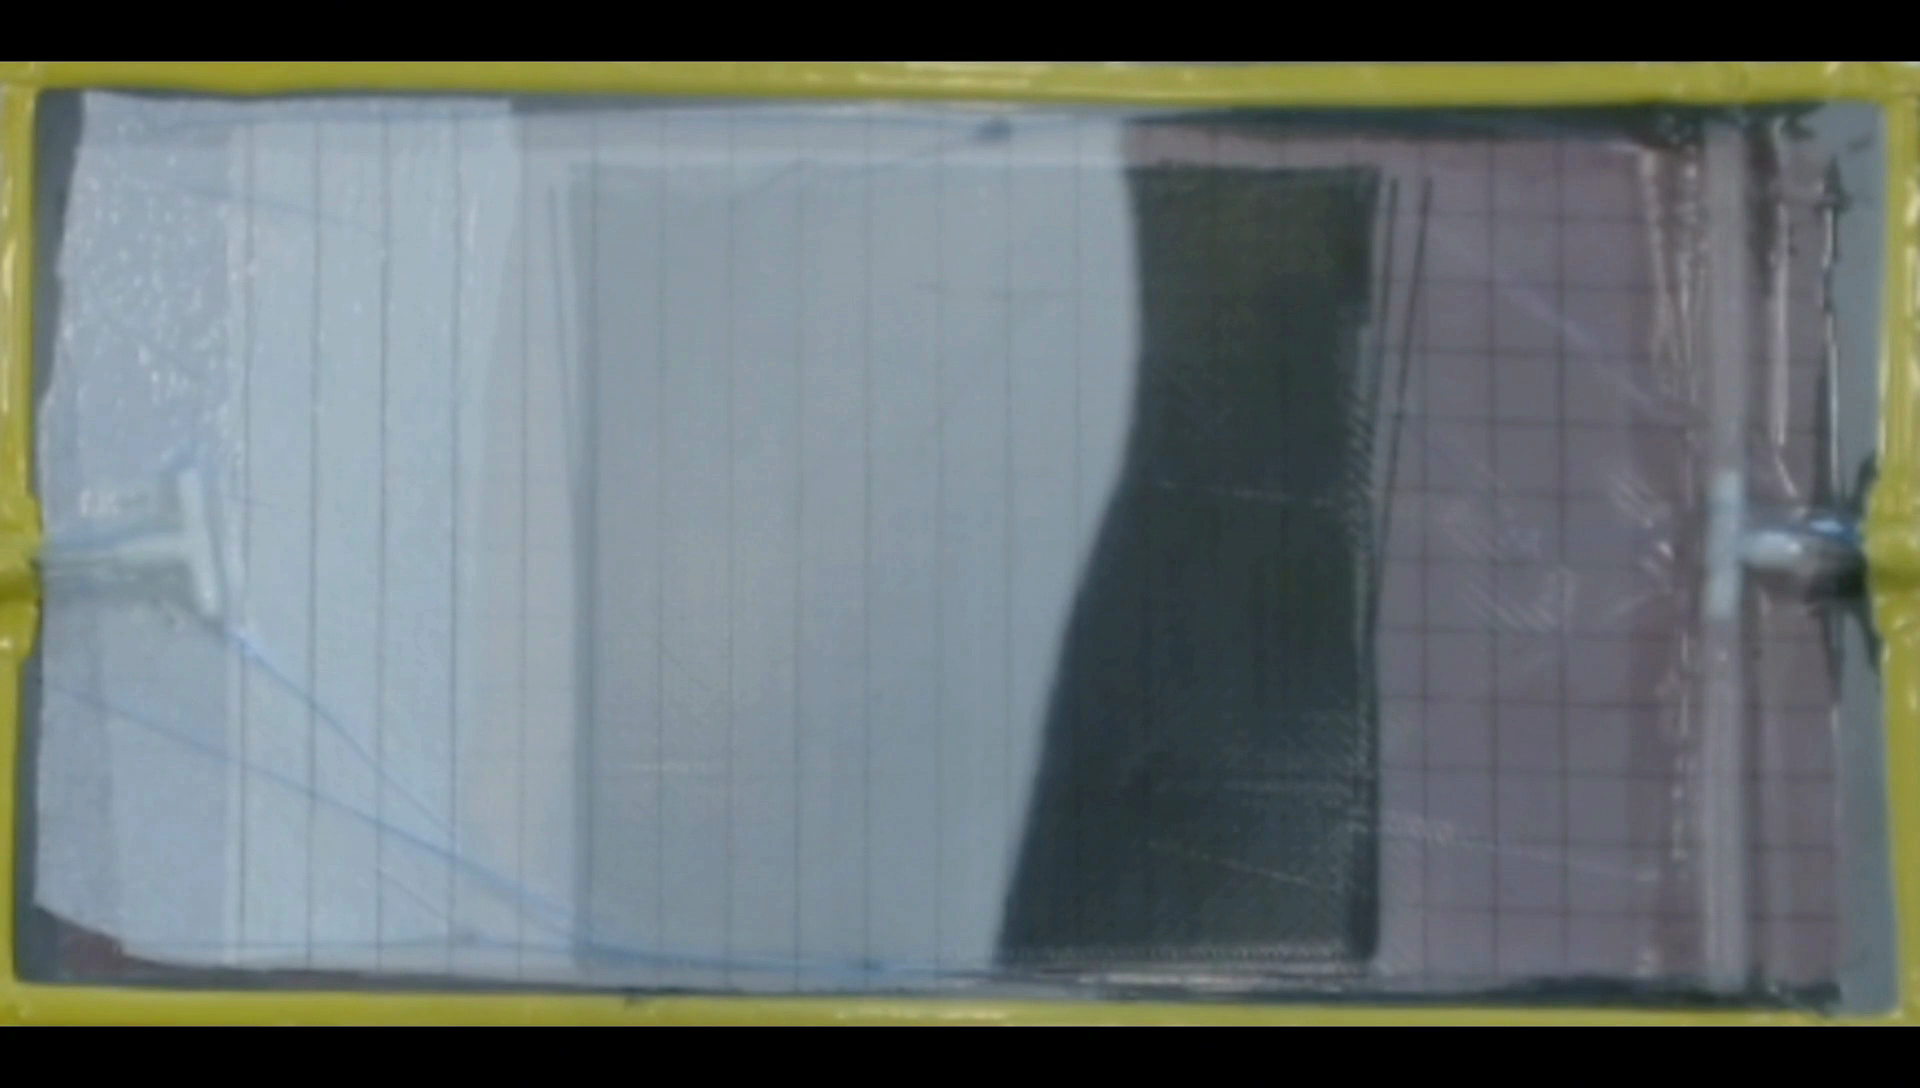
\includegraphics[width=\textwidth]{figures/corrected_frame_024.png}
    \caption{Corrected, frame 24}
\end{subfigure}
\caption{Visual comparison at exposure event $E_1$ (frames 22--24). Top row: original video showing brightness jump at frame 23 where the camera increased exposure by 8\%. Bottom row: corrected video with smooth luminosity transition. The resin flow-front is visible in the lower-left region progressing naturally across all frames in the corrected version.}
\label{fig:visual_comparison_e1}
\end{figure*}

\begin{figure*}[t]
\centering
\begin{subfigure}[b]{0.32\textwidth}
    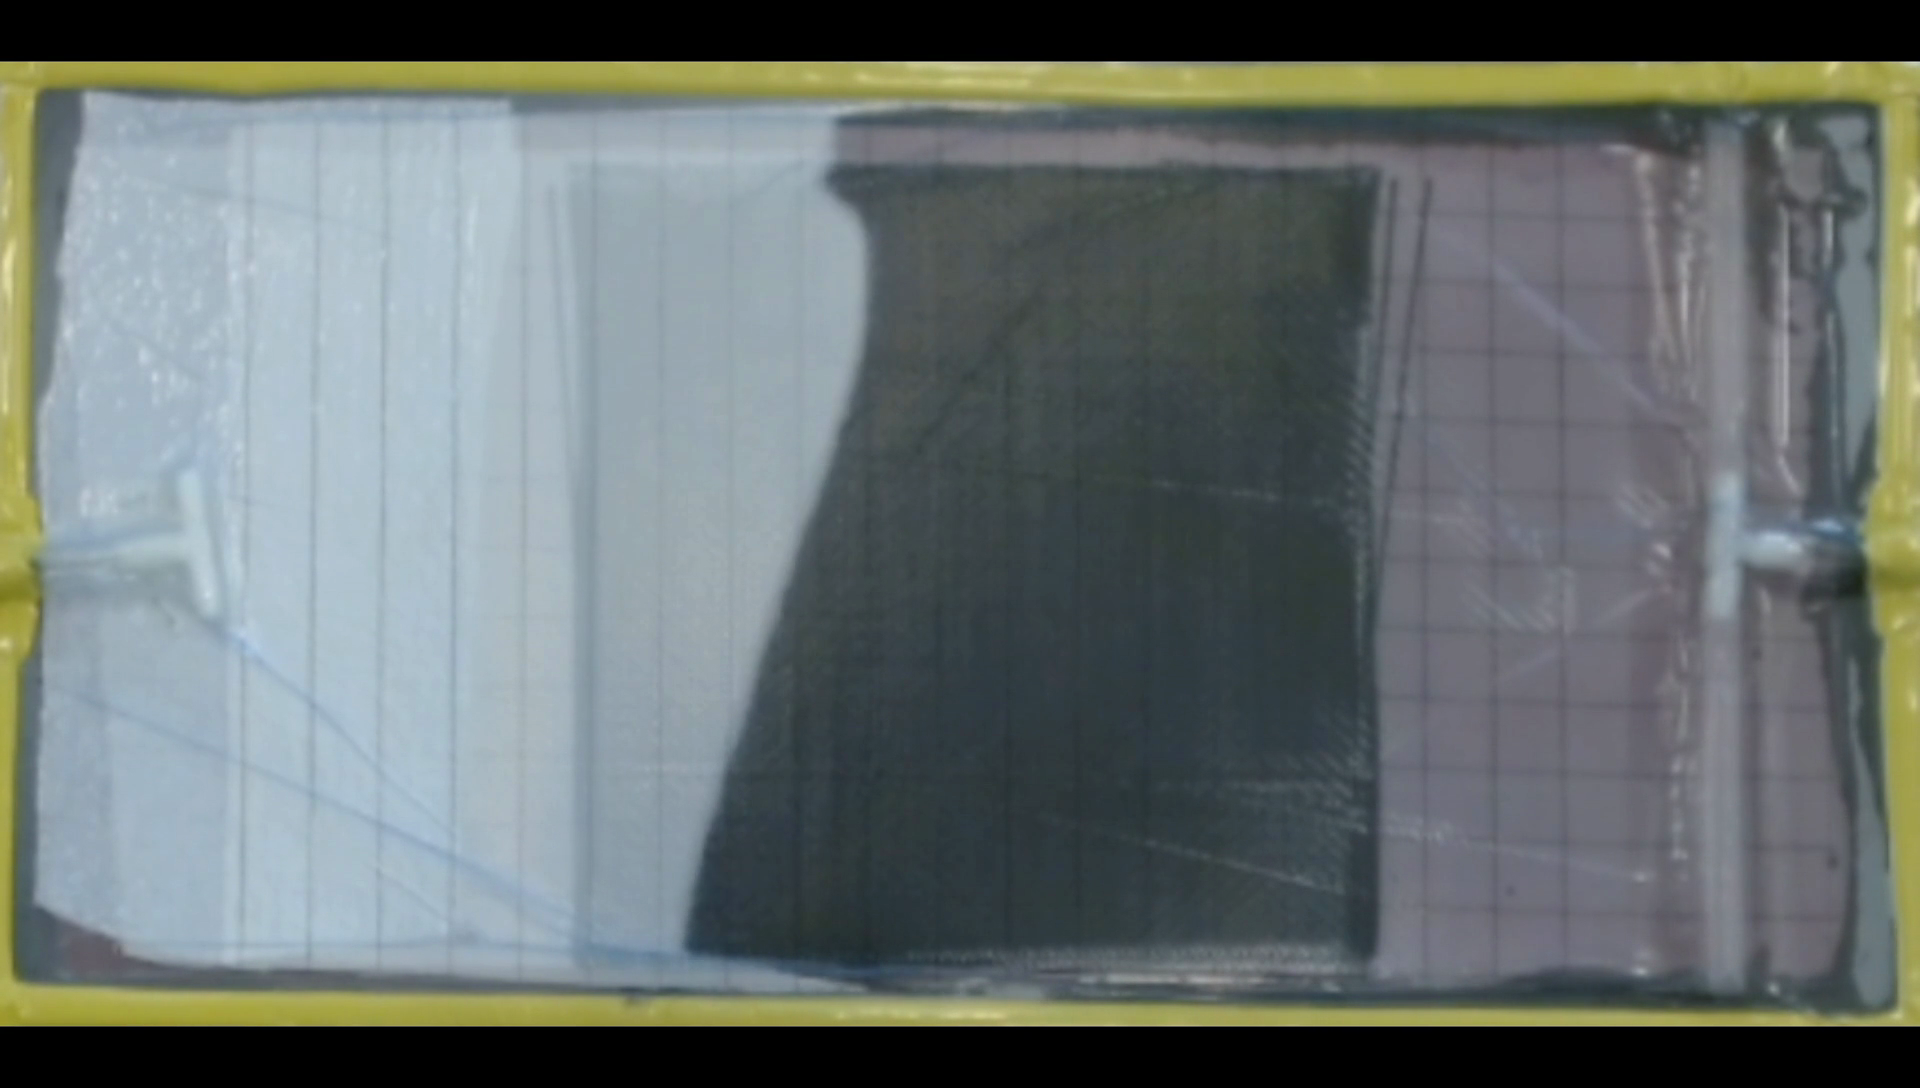
\includegraphics[width=\textwidth]{figures/original_frame_054.png}
    \caption{Original, frame 54}
\end{subfigure}
\hfill
\begin{subfigure}[b]{0.32\textwidth}
    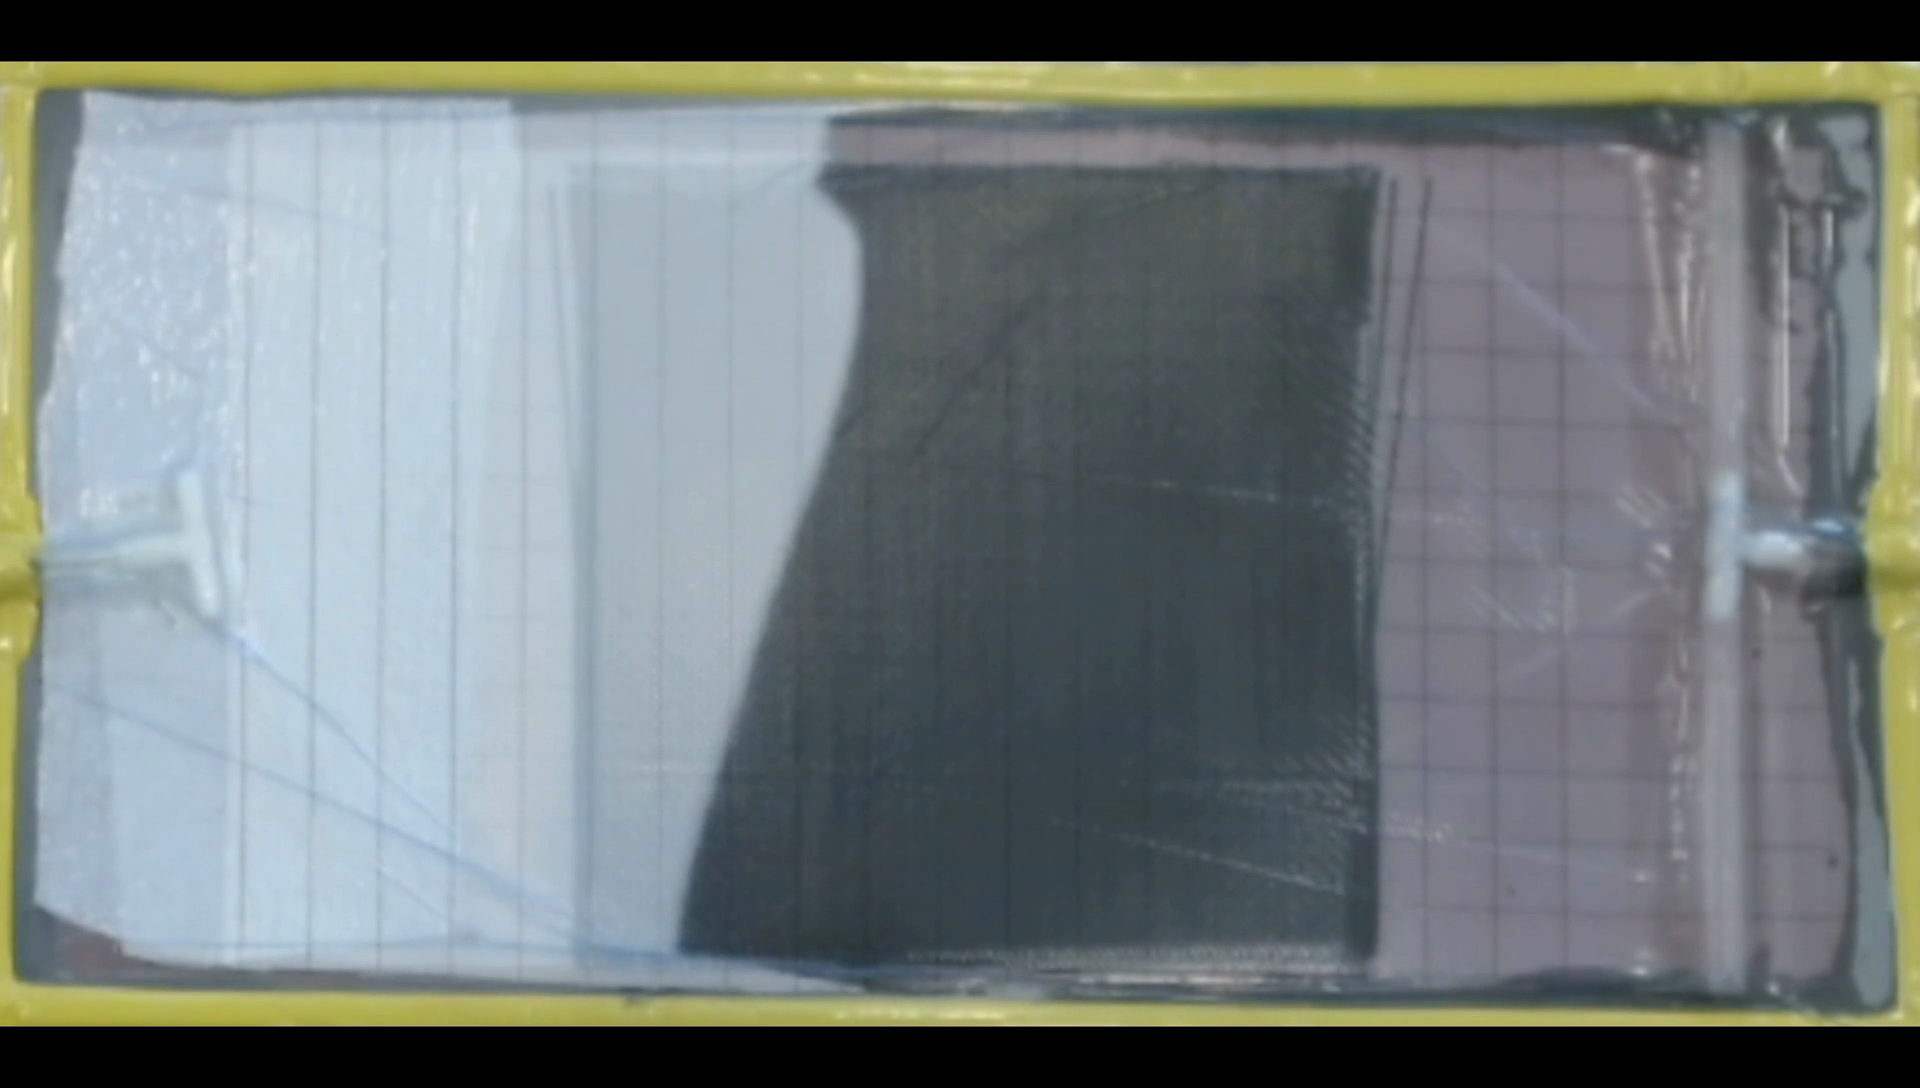
\includegraphics[width=\textwidth]{figures/original_frame_055.png}
    \caption{Original, frame 55 (event)}
\end{subfigure}
\hfill
\begin{subfigure}[b]{0.32\textwidth}
    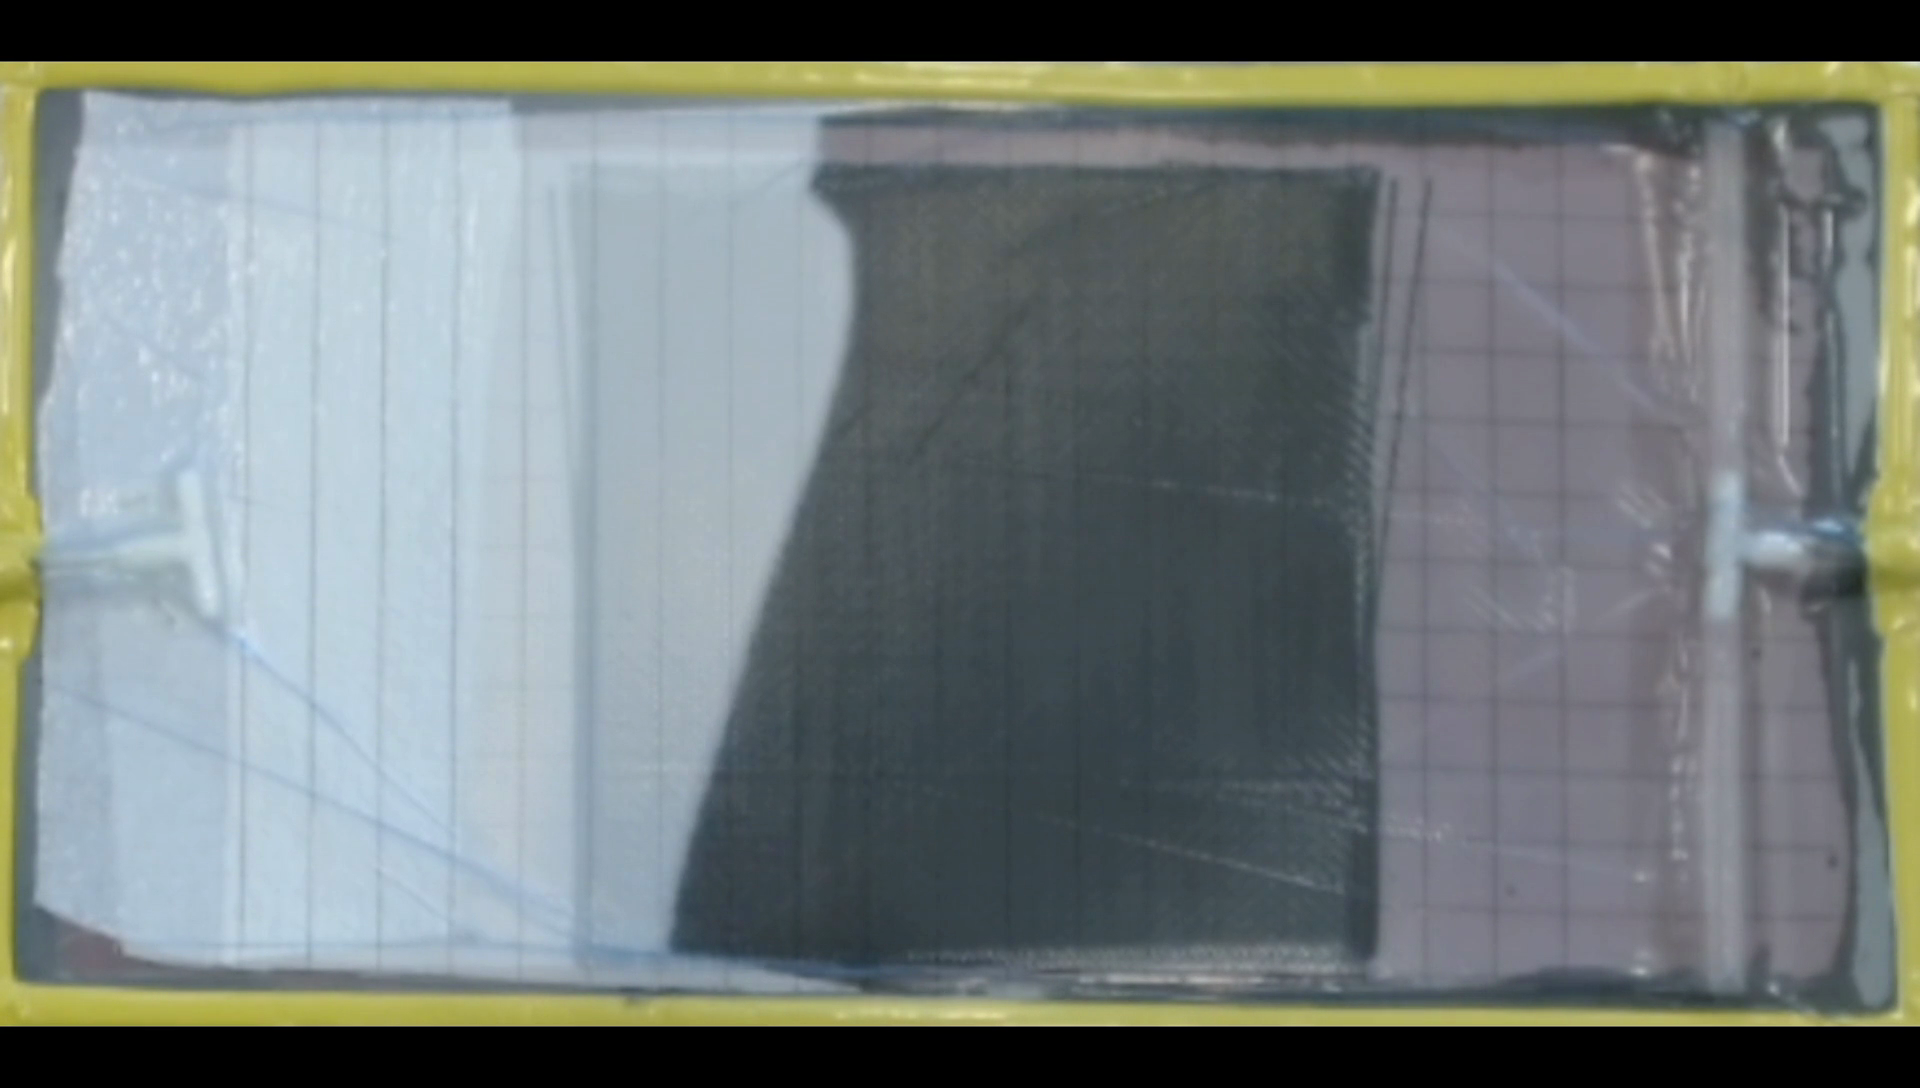
\includegraphics[width=\textwidth]{figures/original_frame_056.png}
    \caption{Original, frame 56}
\end{subfigure}
\\[0.5em]
\begin{subfigure}[b]{0.32\textwidth}
    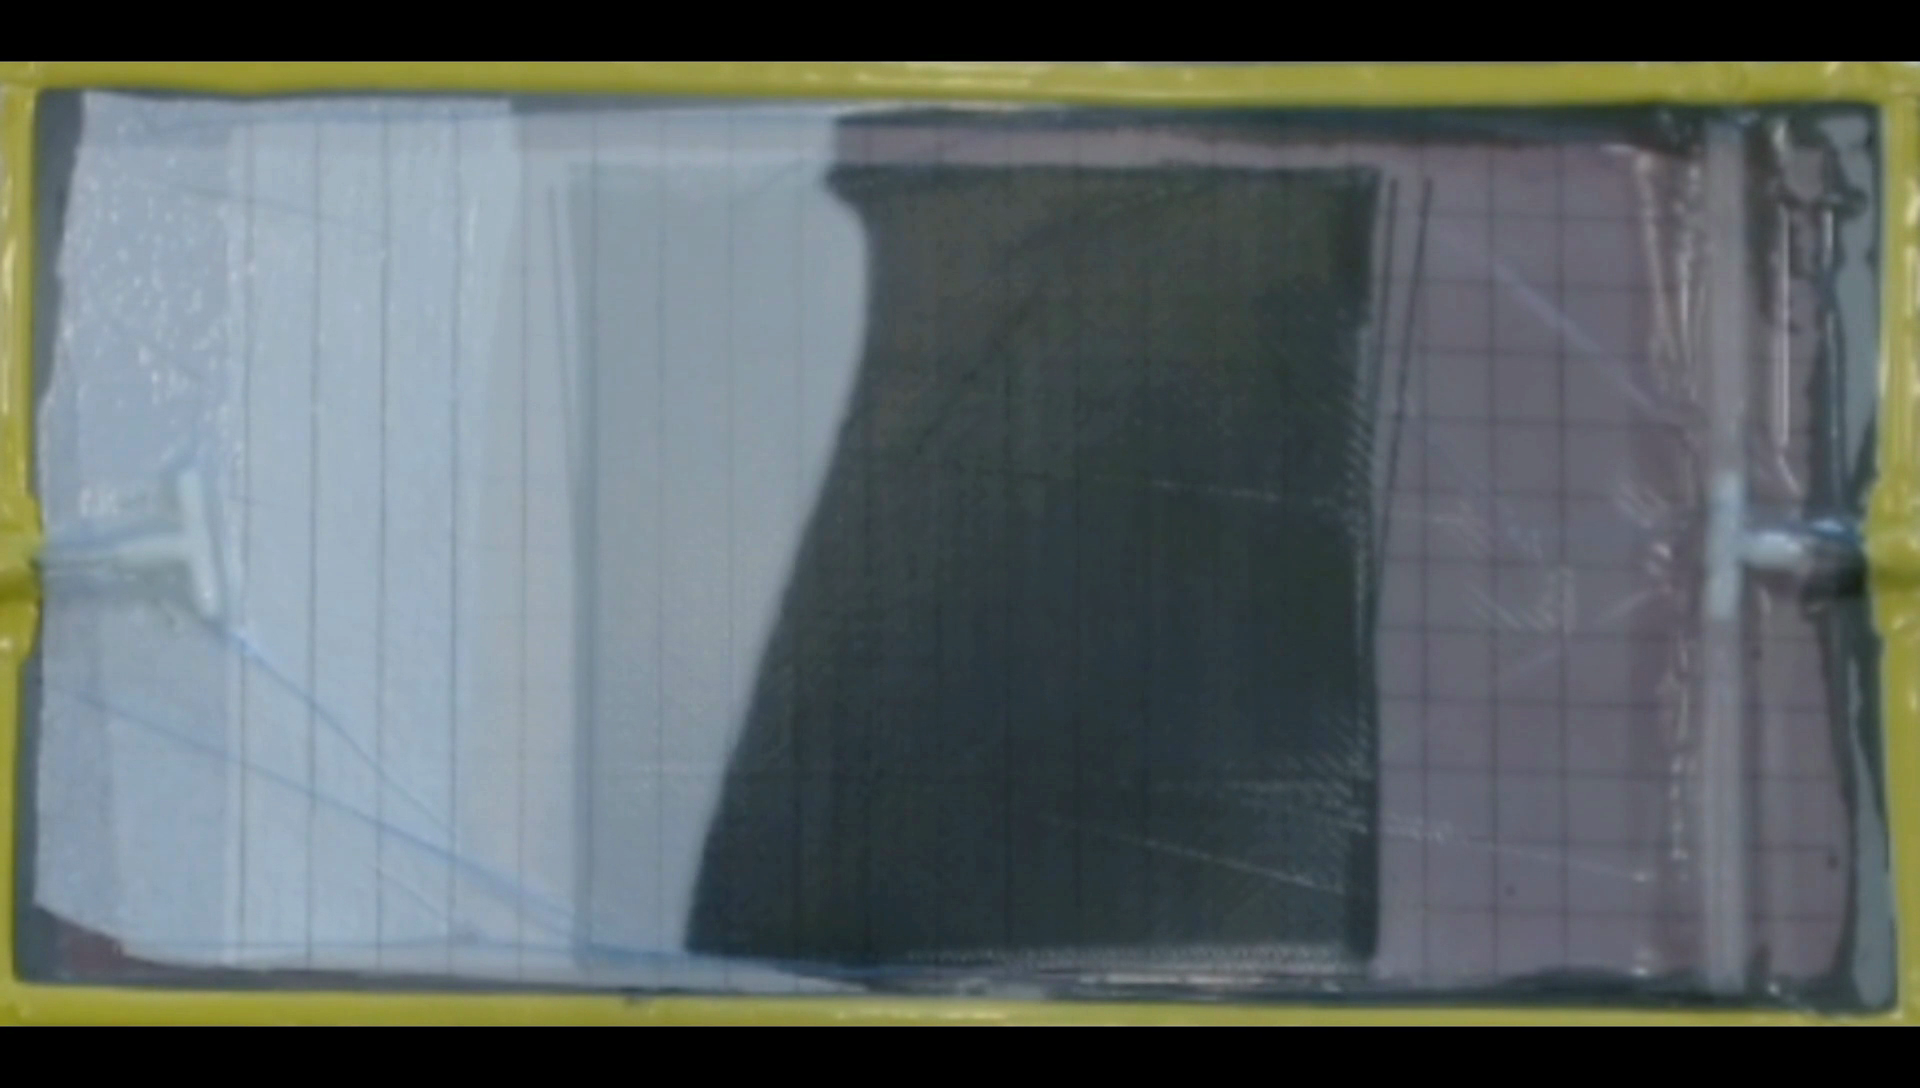
\includegraphics[width=\textwidth]{figures/corrected_frame_054.png}
    \caption{Corrected, frame 54}
\end{subfigure}
\hfill
\begin{subfigure}[b]{0.32\textwidth}
    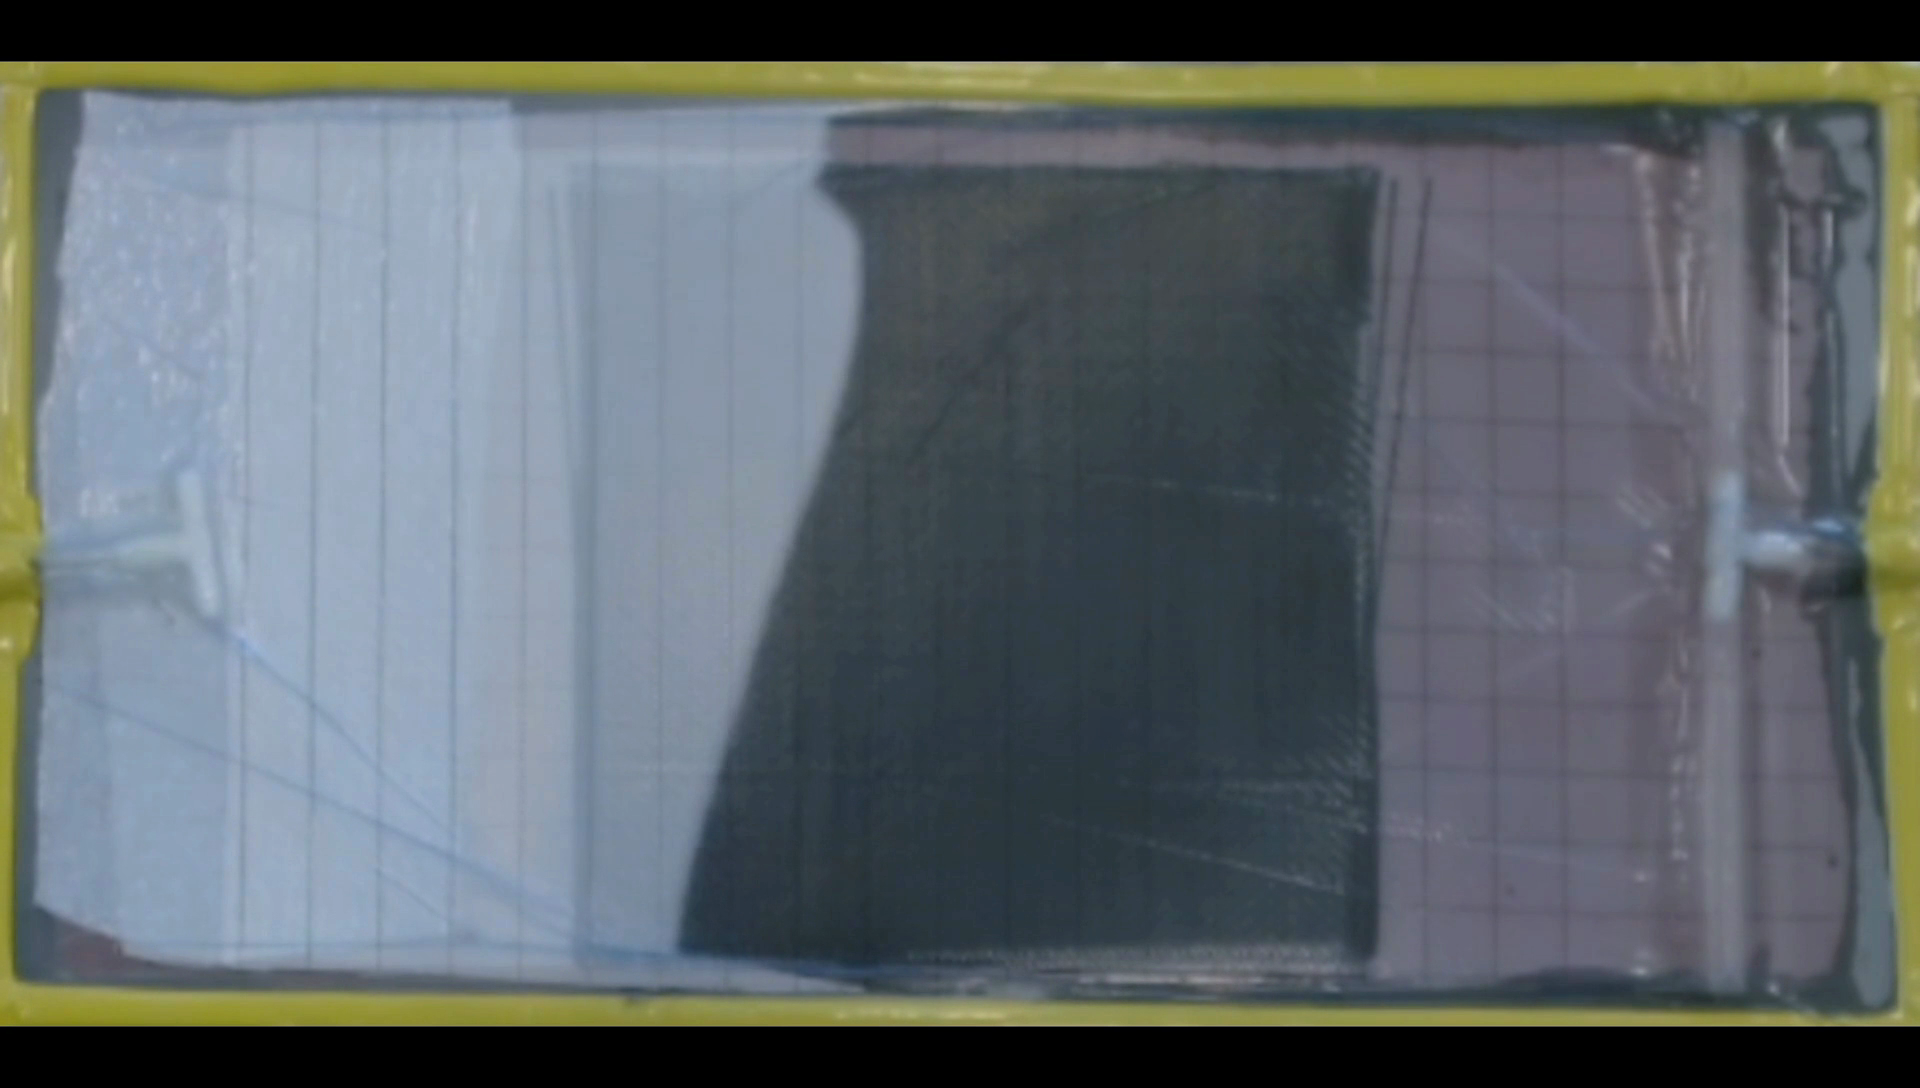
\includegraphics[width=\textwidth]{figures/corrected_frame_055.png}
    \caption{Corrected, frame 55}
\end{subfigure}
\hfill
\begin{subfigure}[b]{0.32\textwidth}
    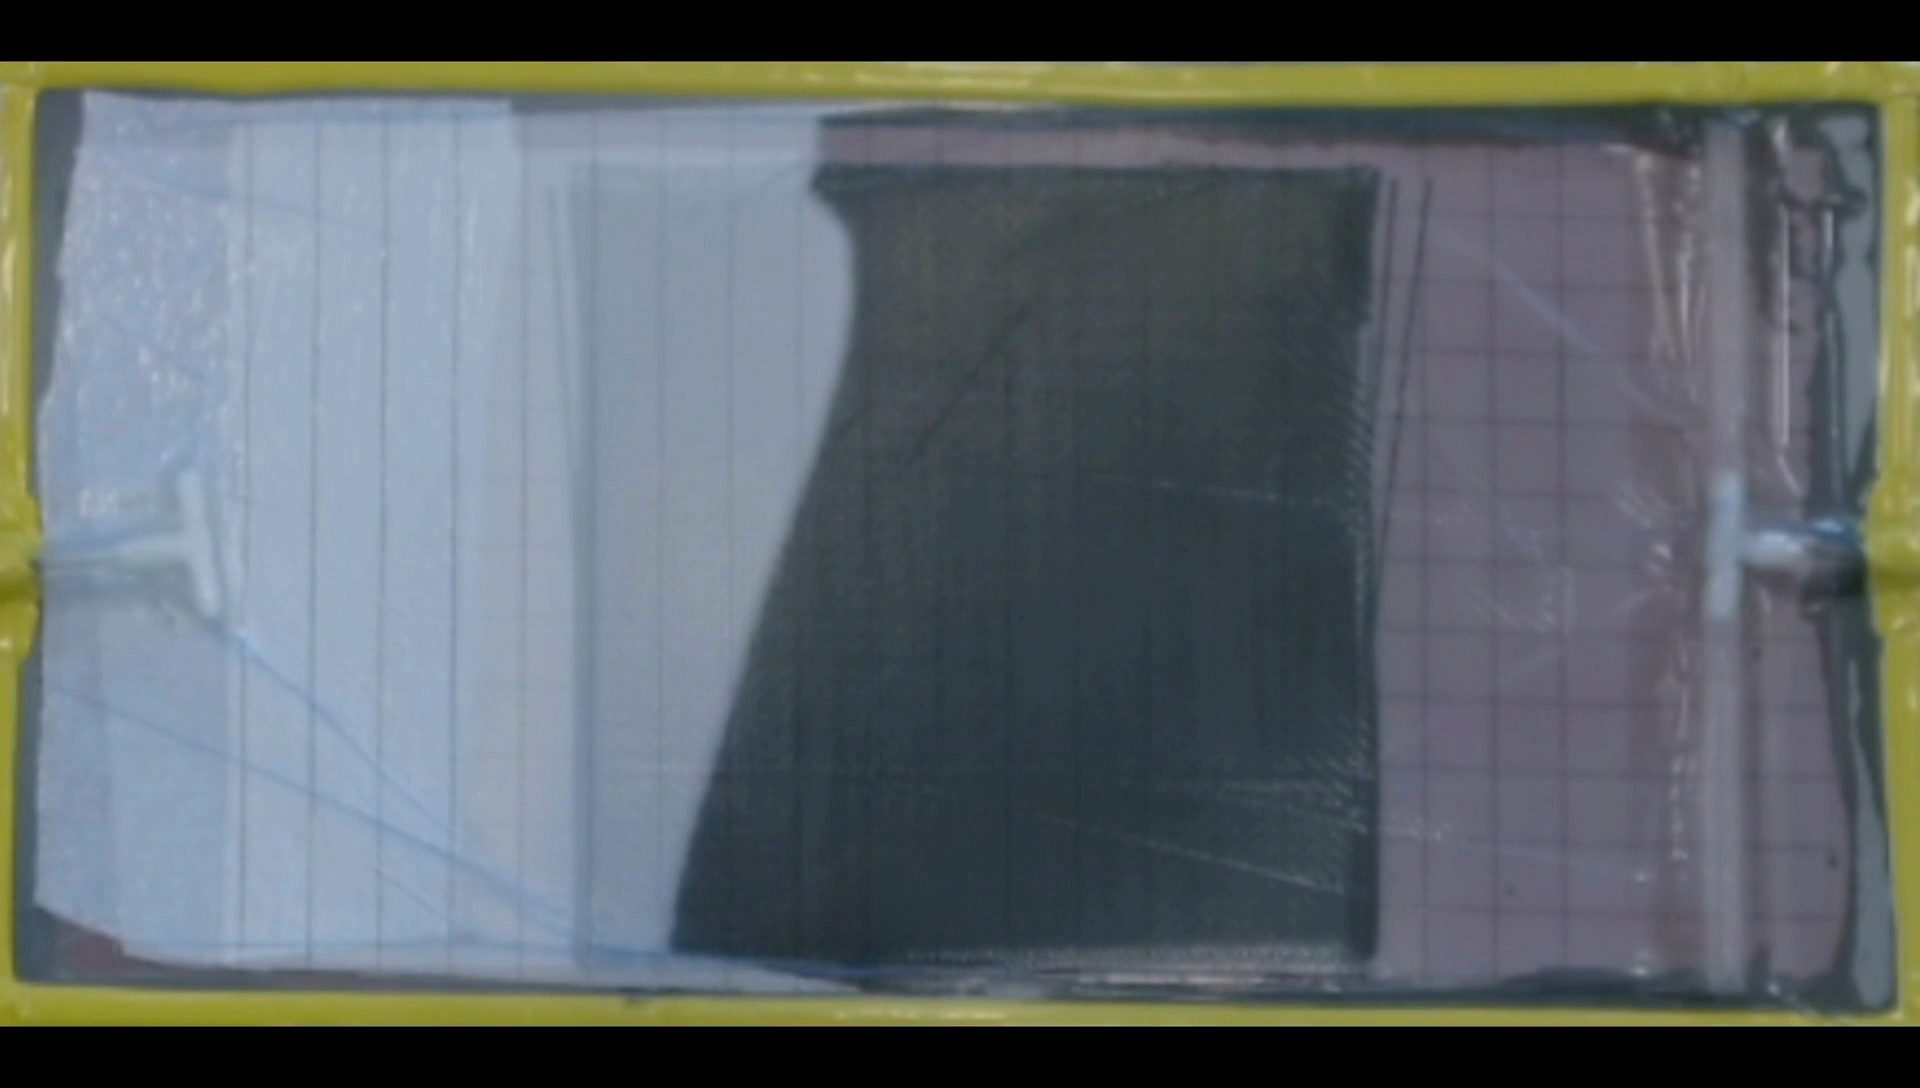
\includegraphics[width=\textwidth]{figures/corrected_frame_056.png}
    \caption{Corrected, frame 56}
\end{subfigure}
\caption{Visual comparison at exposure event $E_2$ (frames 54--56). Top row: original video with visible brightness jump at frame 55 where exposure increased by 9.3\%. Bottom row: corrected video with smooth transition. The resin flow-front has progressed significantly from $E_1$, covering approximately 30\% of the visible area.}
\label{fig:visual_comparison_e2}
\end{figure*}

\begin{figure*}[t]
\centering
\begin{subfigure}[b]{0.32\textwidth}
    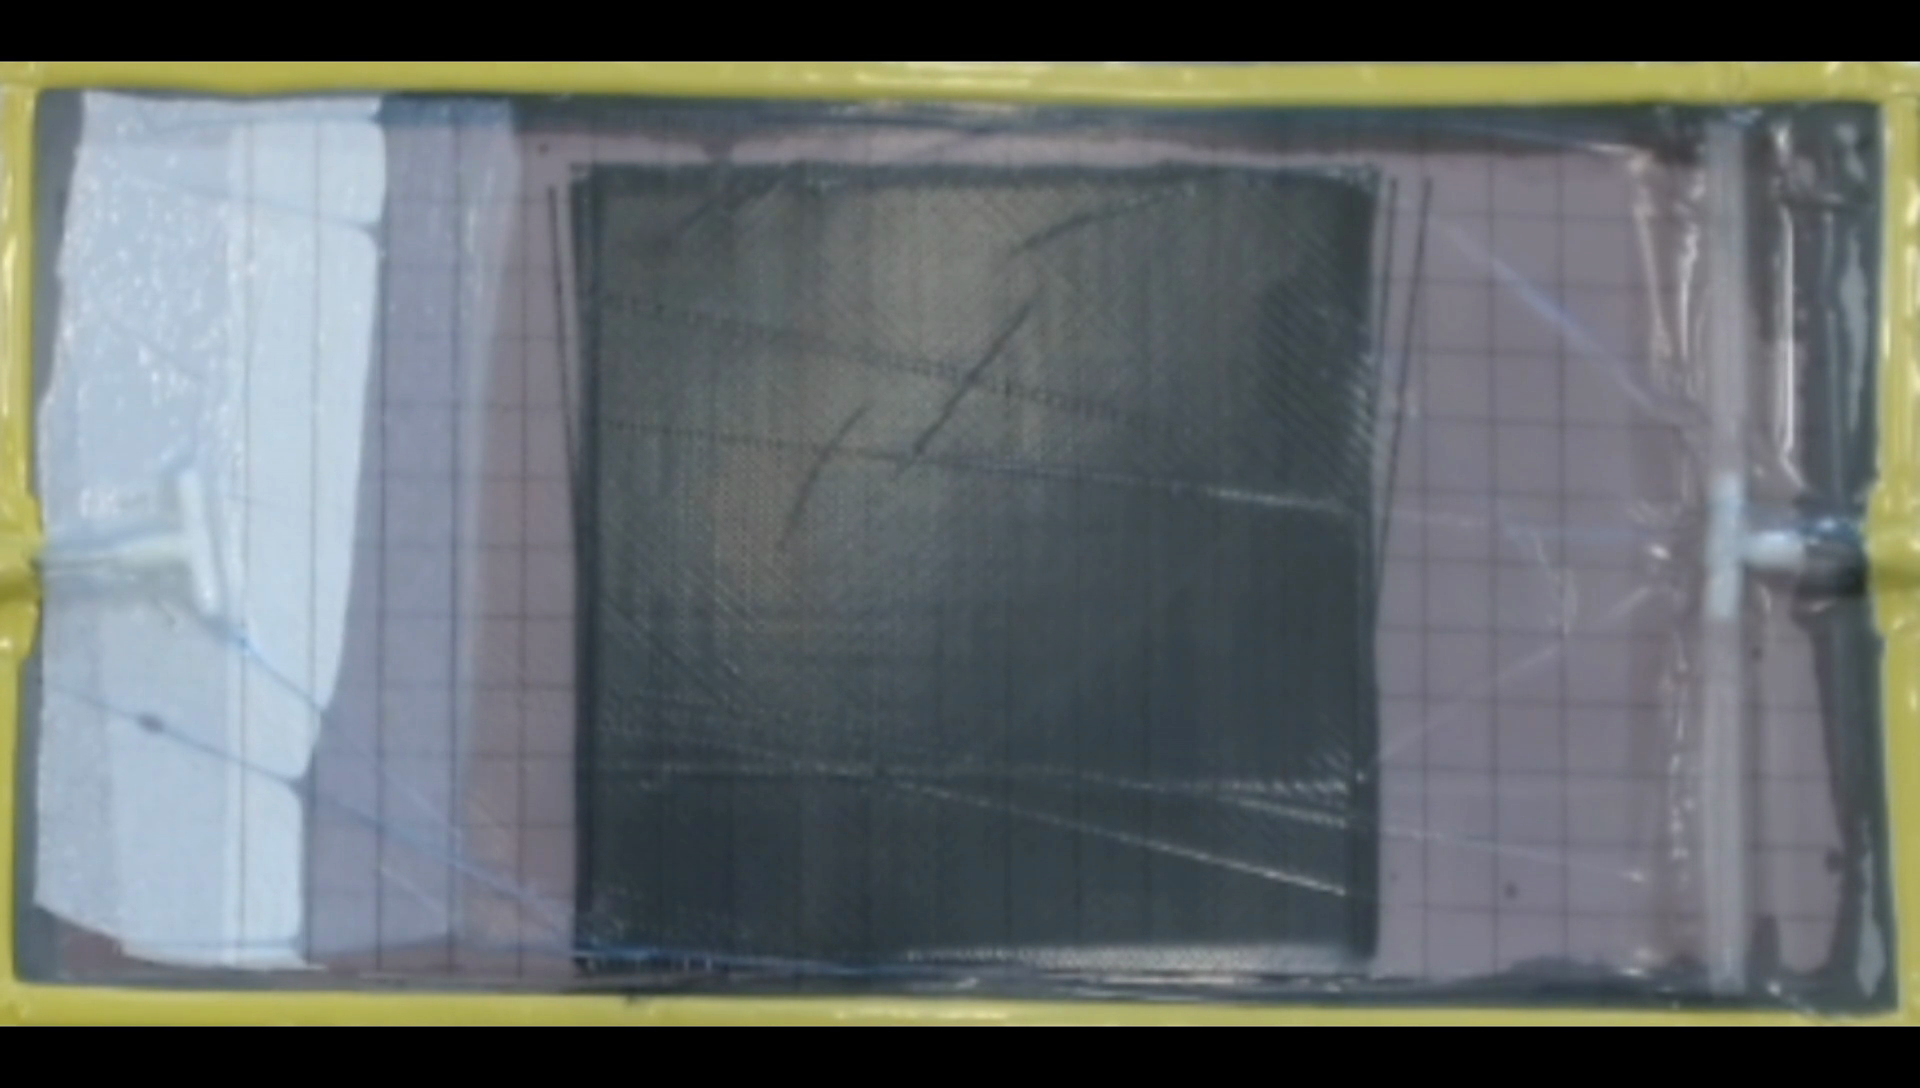
\includegraphics[width=\textwidth]{figures/original_frame_128.png}
    \caption{Original, frame 128}
\end{subfigure}
\hfill
\begin{subfigure}[b]{0.32\textwidth}
    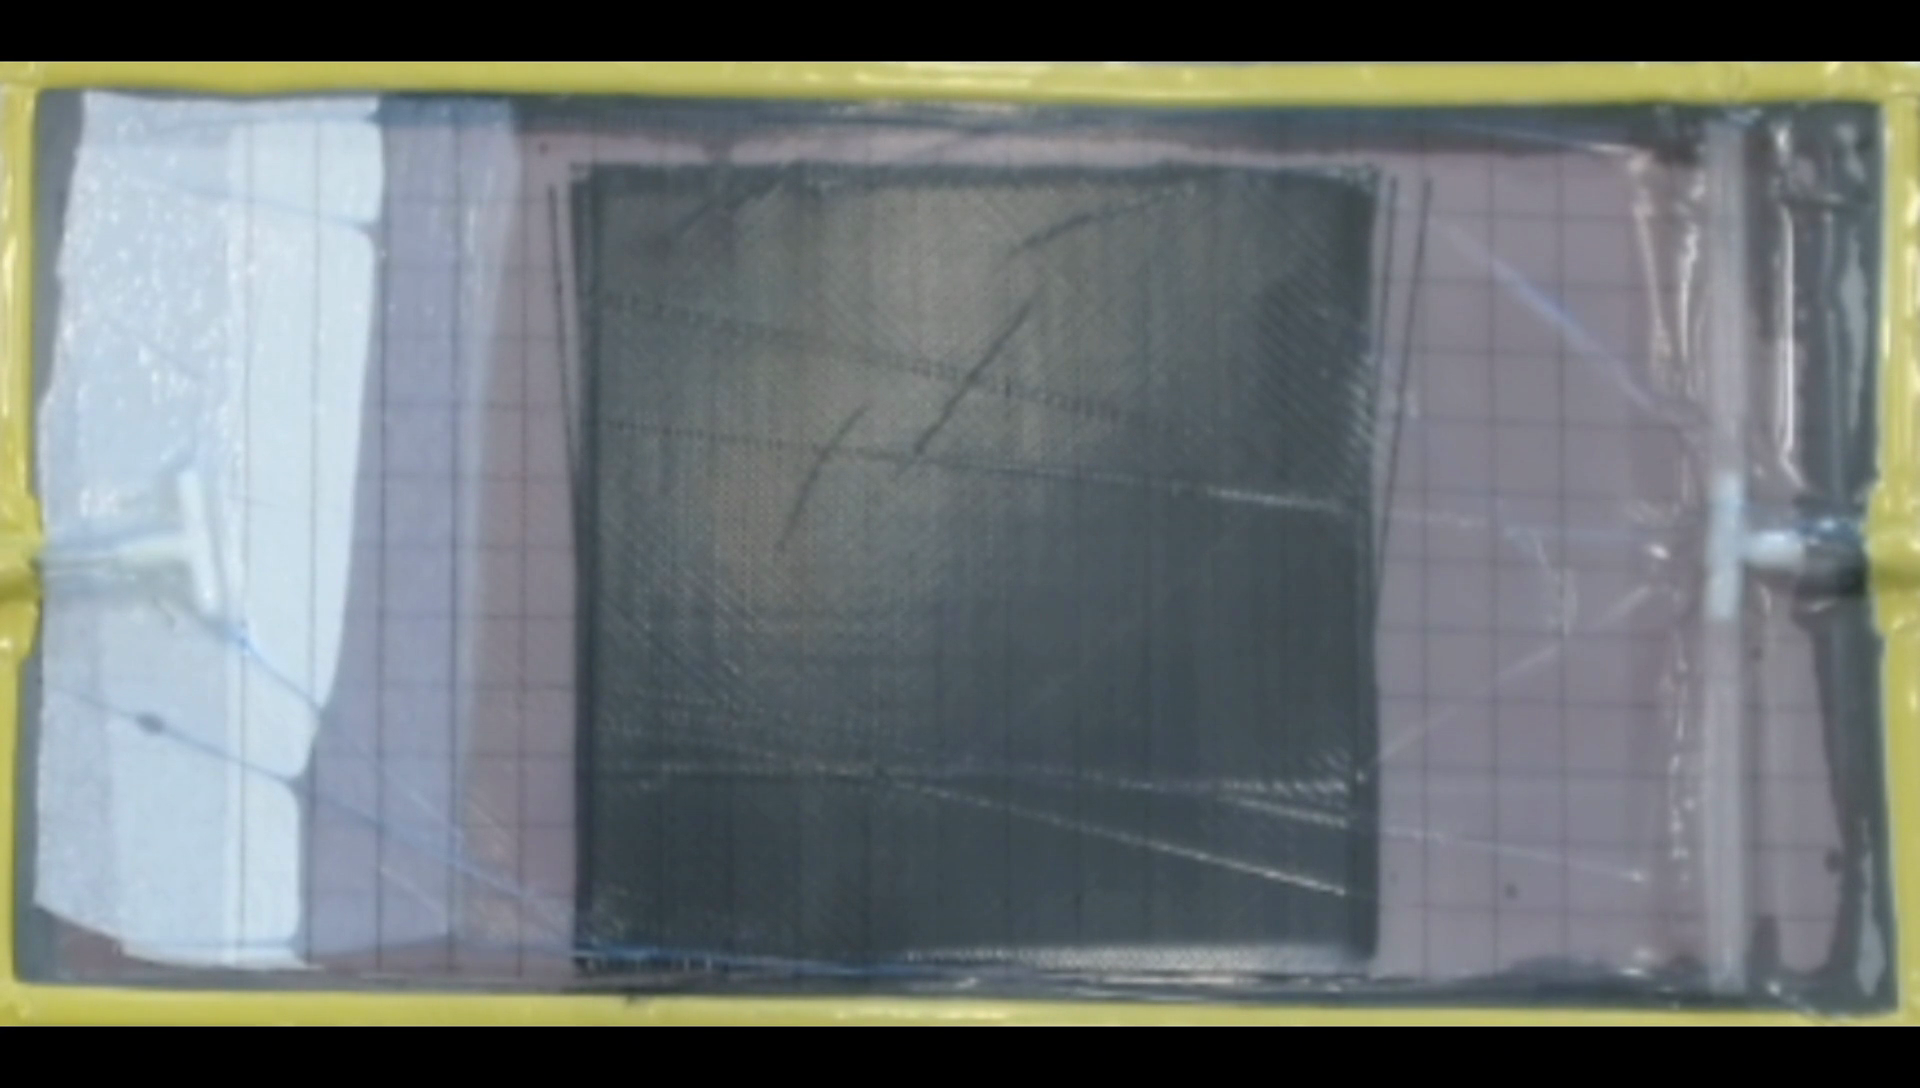
\includegraphics[width=\textwidth]{figures/original_frame_129.png}
    \caption{Original, frame 129 (event)}
\end{subfigure}
\hfill
\begin{subfigure}[b]{0.32\textwidth}
    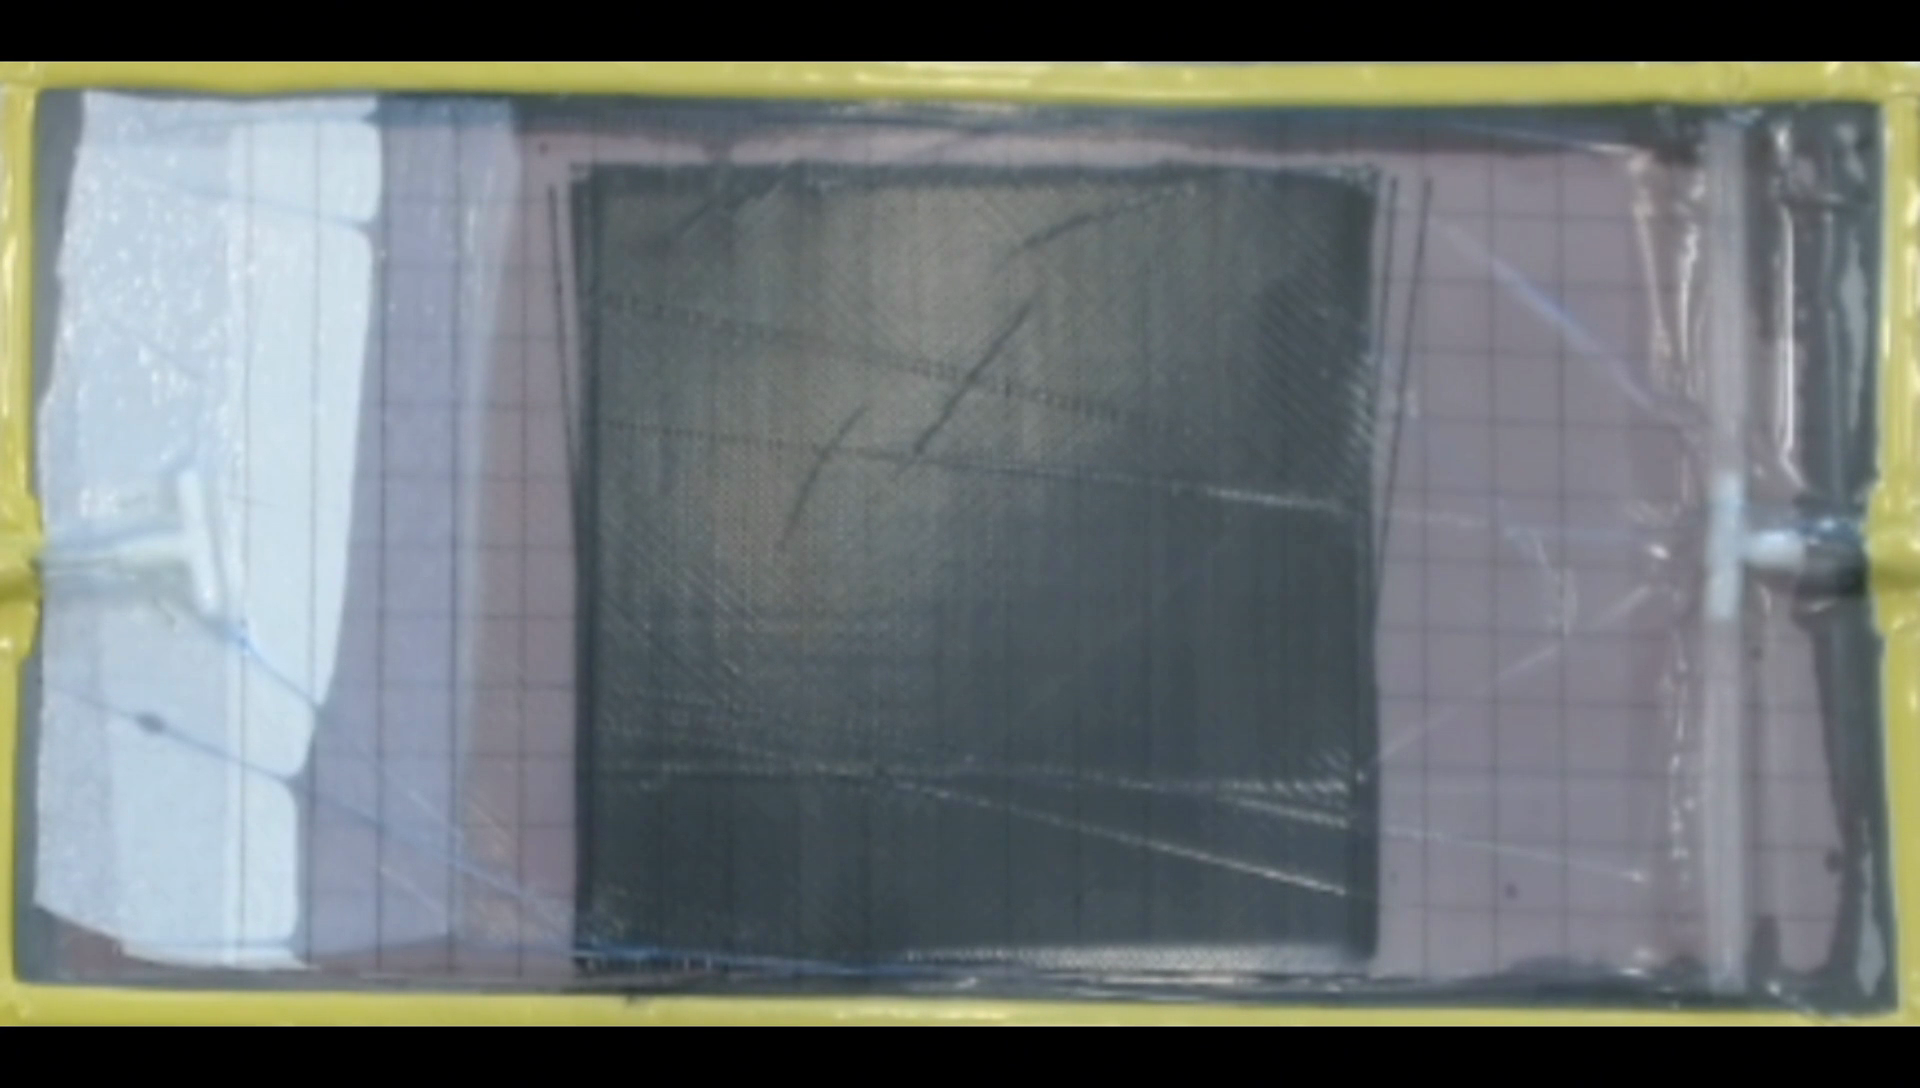
\includegraphics[width=\textwidth]{figures/original_frame_130.png}
    \caption{Original, frame 130}
\end{subfigure}
\\[0.5em]
\begin{subfigure}[b]{0.32\textwidth}
    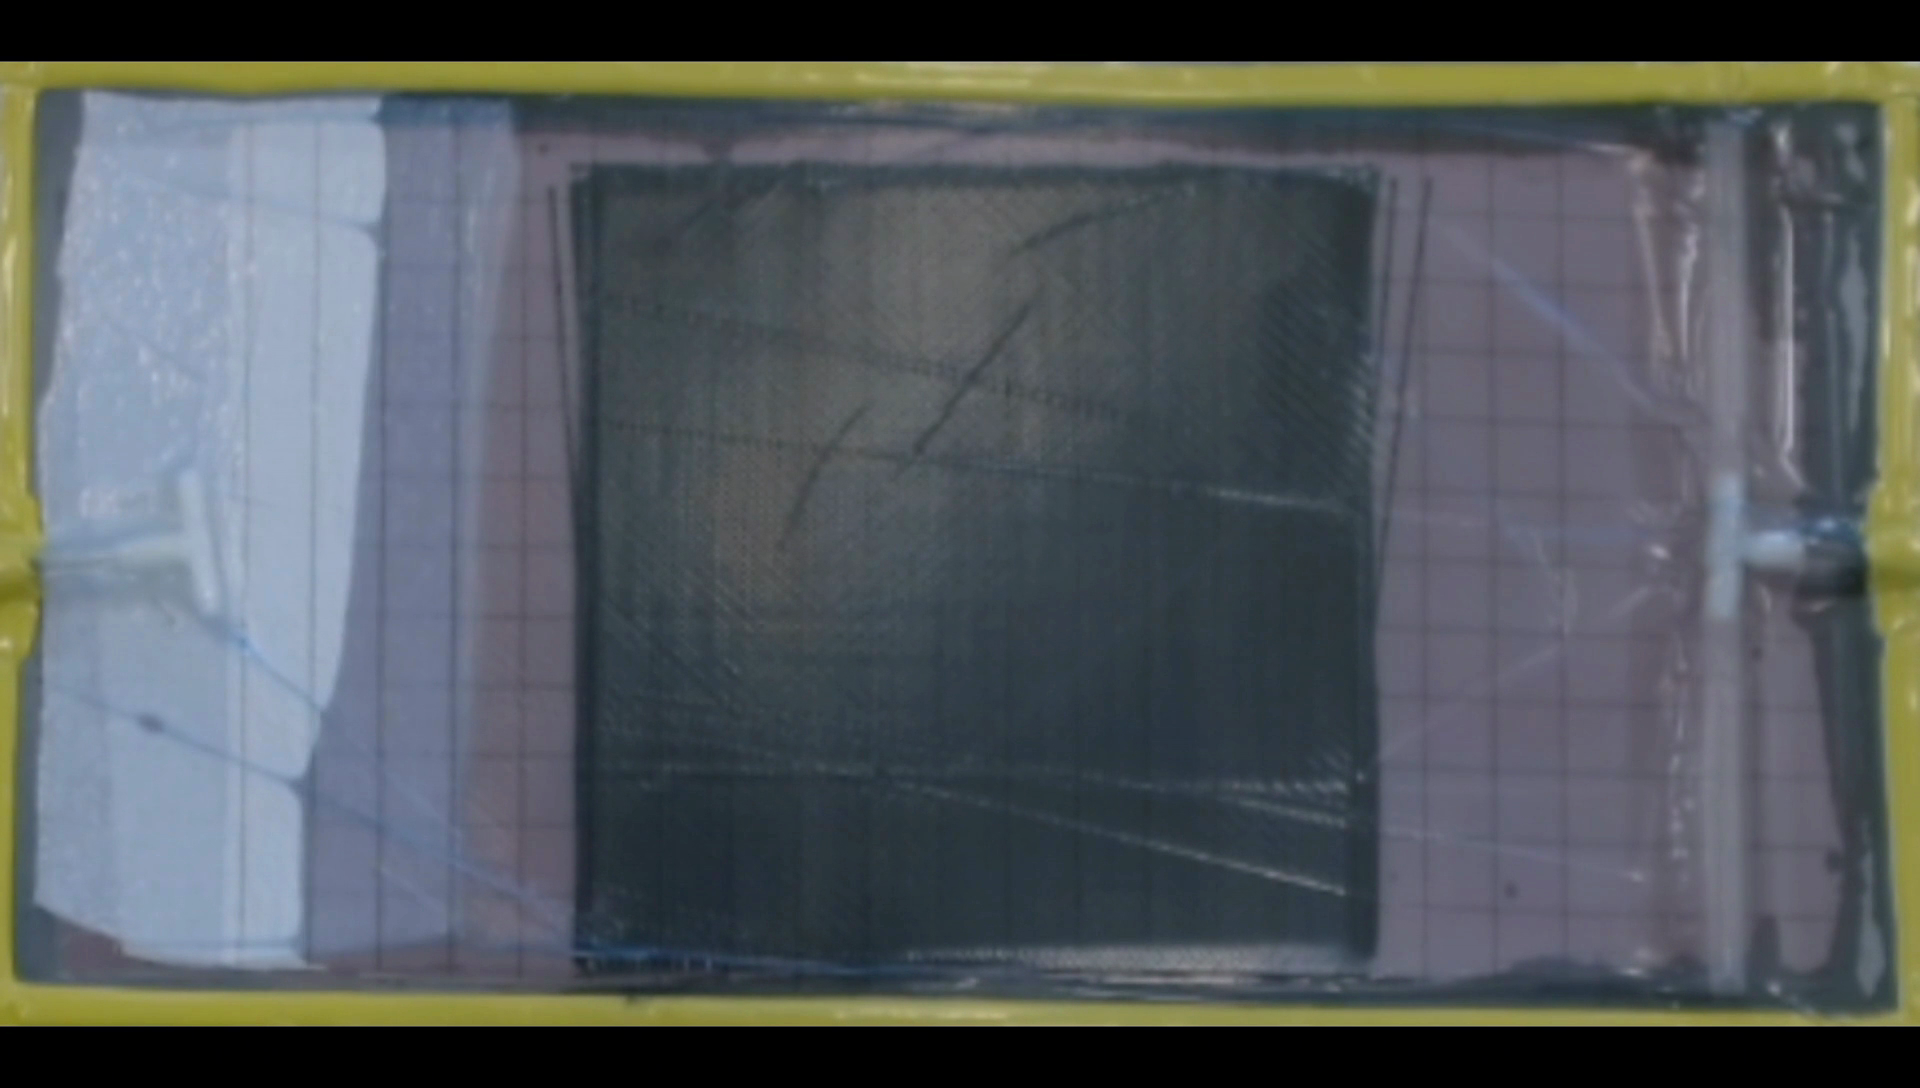
\includegraphics[width=\textwidth]{figures/corrected_frame_128.png}
    \caption{Corrected, frame 128}
\end{subfigure}
\hfill
\begin{subfigure}[b]{0.32\textwidth}
    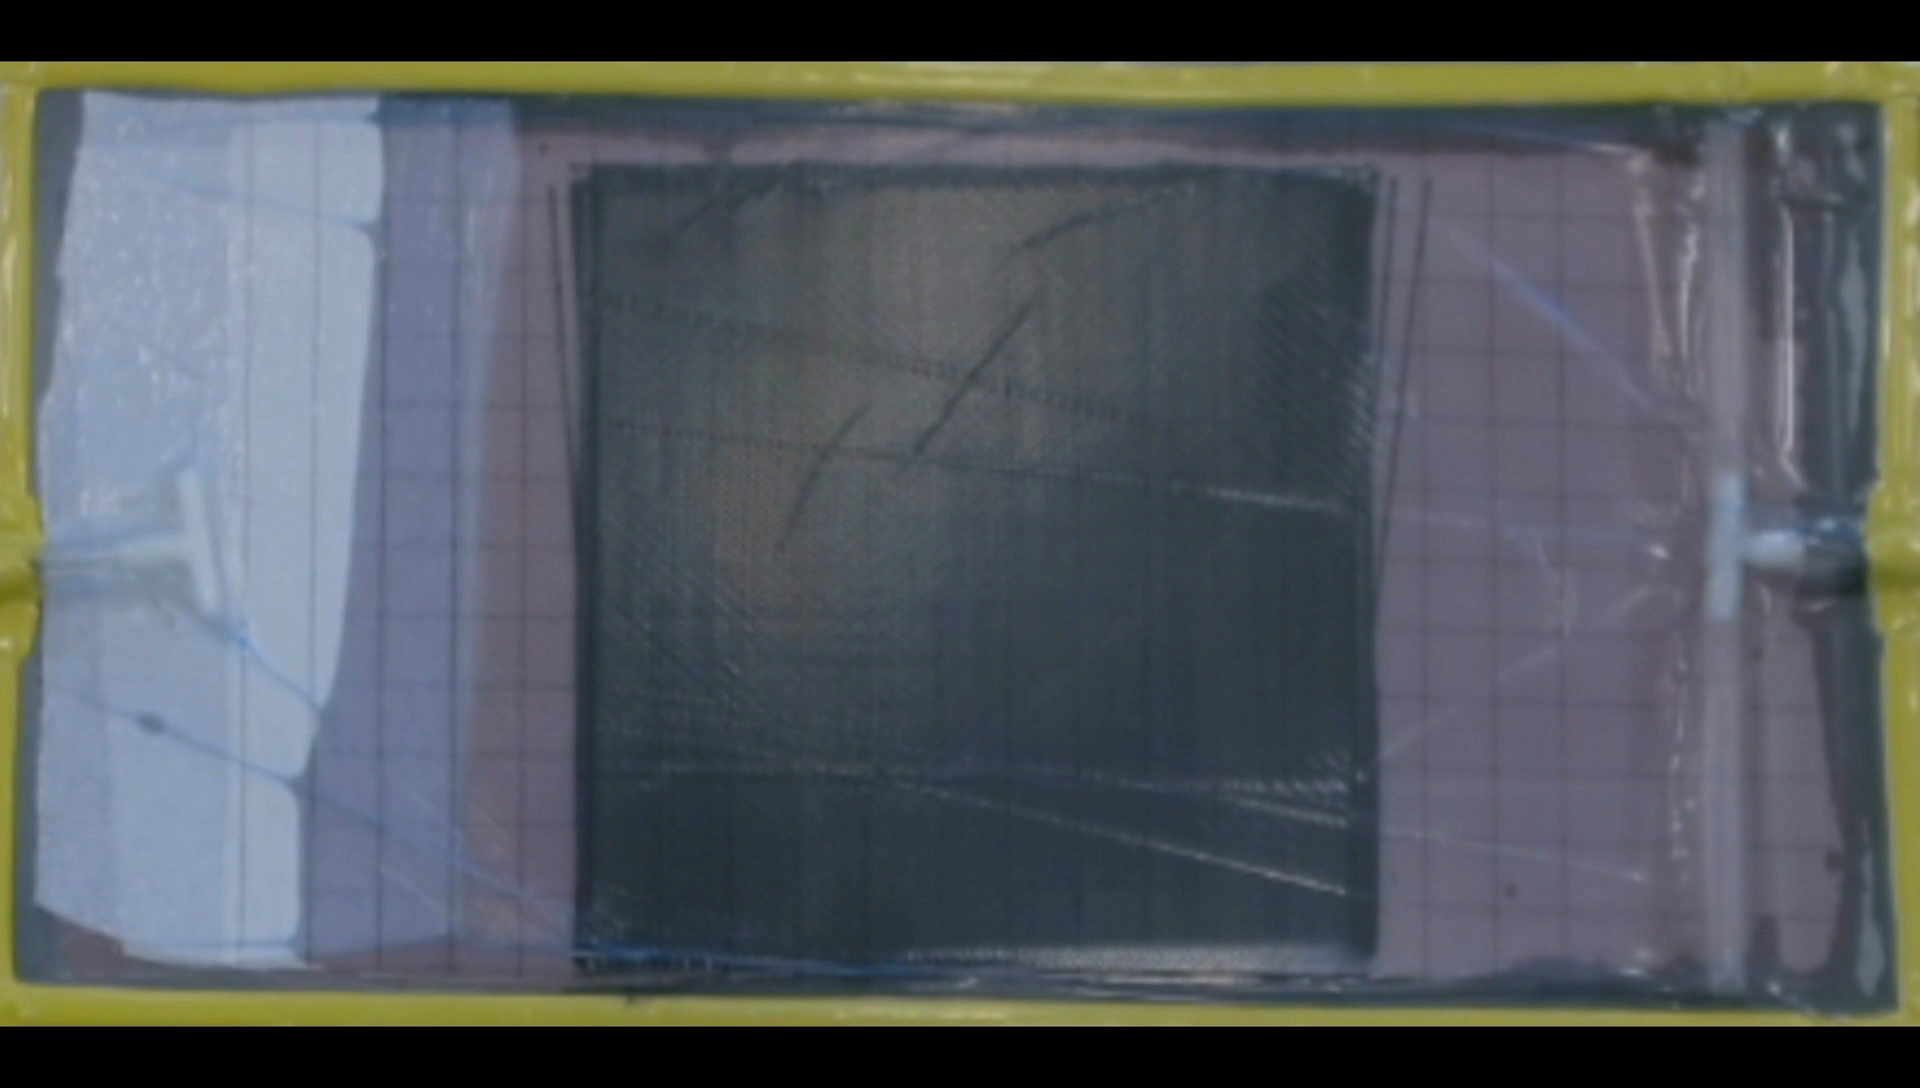
\includegraphics[width=\textwidth]{figures/corrected_frame_129.png}
    \caption{Corrected, frame 129}
\end{subfigure}
\hfill
\begin{subfigure}[b]{0.32\textwidth}
    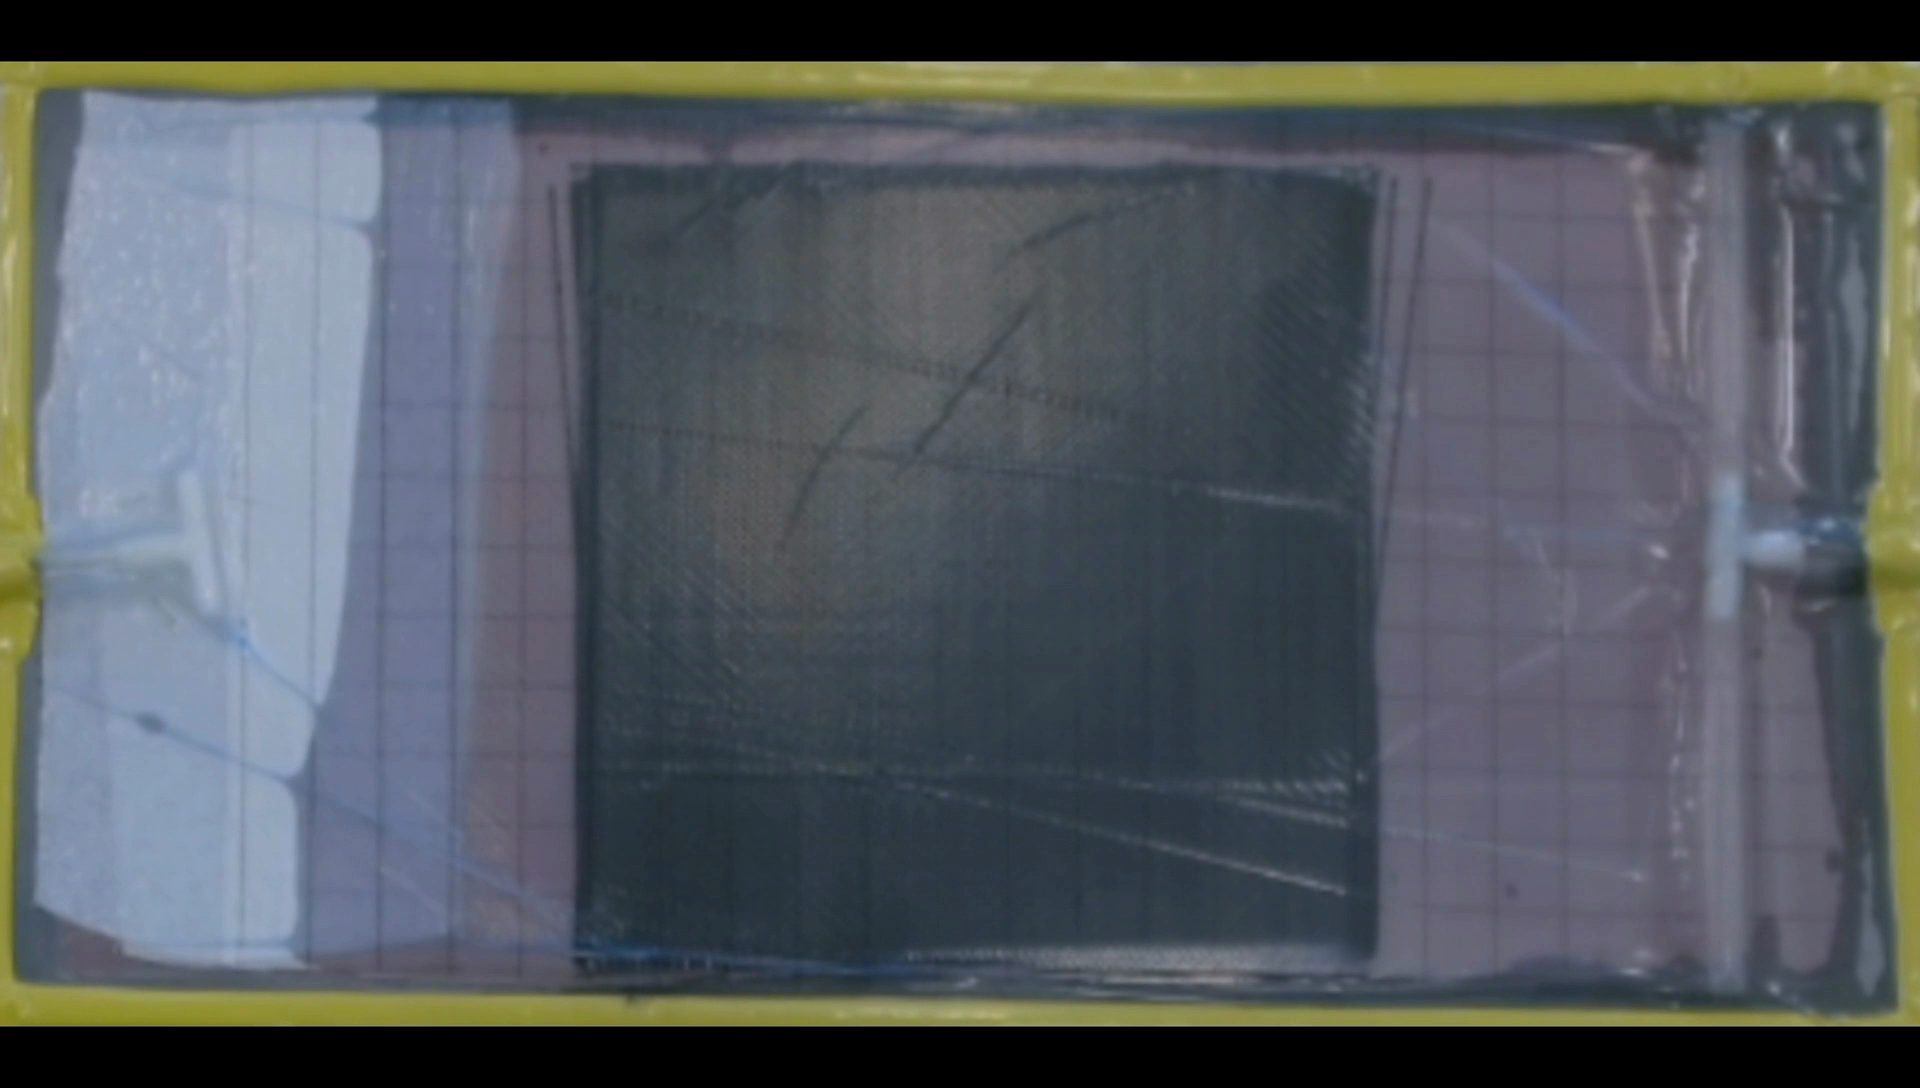
\includegraphics[width=\textwidth]{figures/corrected_frame_130.png}
    \caption{Corrected, frame 130}
\end{subfigure}
\caption{Visual comparison at exposure event $E_3$ (frames 128--130). Top row: original video with brightness discontinuity at frame 129 where exposure increased by 8.6\%. Bottom row: corrected video eliminates this artifact while preserving all spatial detail and color relationships. By this point, resin covers approximately 65\% of the visible area and the cumulative correction factor reaches 0.780.}
\label{fig:visual_comparison_e3}
\end{figure*}

\subsection{Color Preservation Analysis}

Figure~\ref{fig:color_preservation} shows the color ratio comparison across correction methods.

\begin{figure*}[t]
\centering
\begin{subfigure}[b]{0.48\textwidth}
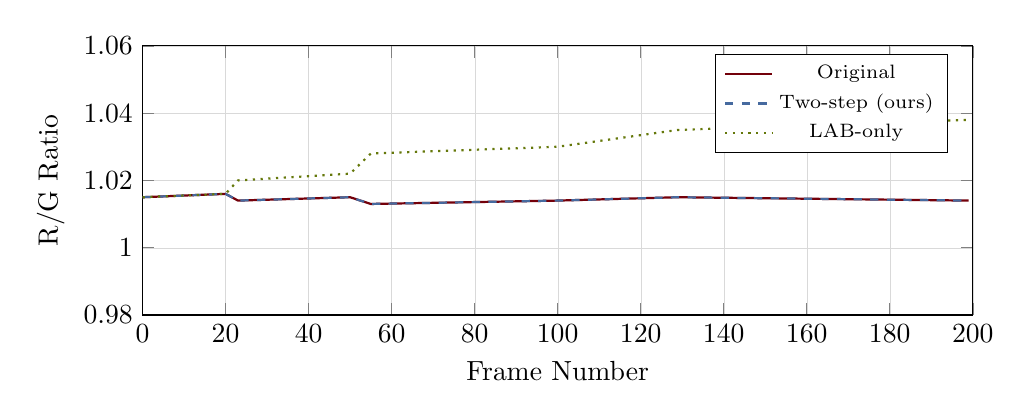
\begin{tikzpicture}
    \begin{axis}[
        width=\textwidth,
        height=5cm,
        xlabel={Frame Number},
        ylabel={R/G Ratio},
        xmin=0, xmax=200,
        ymin=0.98, ymax=1.06,
        grid=both,
        grid style={line width=0.1pt, draw=gray!30},
        legend pos=north east,
        legend style={font=\scriptsize},
    ]
    \addplot[color=garnet, thick, mark=none] coordinates {
        (0,1.015) (20,1.016) (23,1.014) (50,1.015) (55,1.013) (100,1.014) (129,1.015) (199,1.014)
    };
    \addlegendentry{Original}
    \addplot[color=atlantic, thick, mark=none, dashed] coordinates {
        (0,1.015) (20,1.016) (23,1.014) (50,1.015) (55,1.013) (100,1.014) (129,1.015) (199,1.014)
    };
    \addlegendentry{Two-step (ours)}
    \addplot[color=horseshoe, thick, mark=none, dotted] coordinates {
        (0,1.015) (20,1.016) (23,1.020) (50,1.022) (55,1.028) (100,1.030) (129,1.035) (199,1.038)
    };
    \addlegendentry{LAB-only}
    \end{axis}
\end{tikzpicture}
\caption{R/G ratio comparison}
\end{subfigure}
\hfill
\begin{subfigure}[b]{0.48\textwidth}
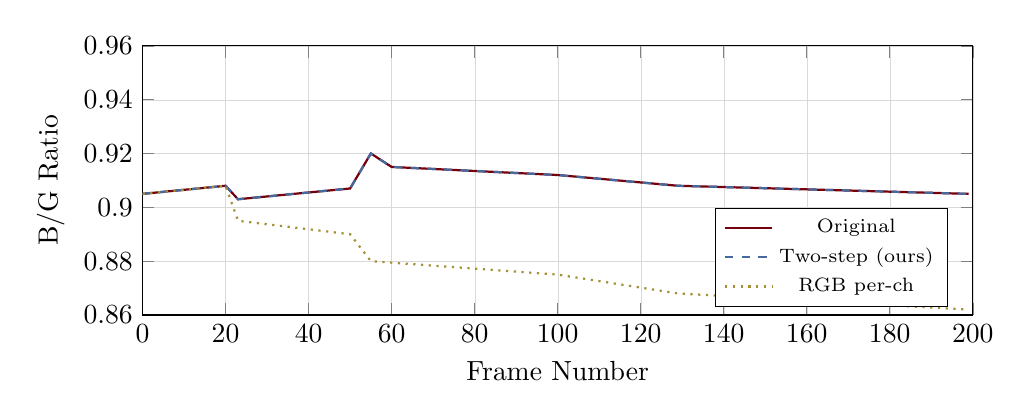
\begin{tikzpicture}
    \begin{axis}[
        width=\textwidth,
        height=5cm,
        xlabel={Frame Number},
        ylabel={B/G Ratio},
        xmin=0, xmax=200,
        ymin=0.86, ymax=0.96,
        grid=both,
        grid style={line width=0.1pt, draw=gray!30},
        legend pos=south east,
        legend style={font=\scriptsize},
    ]
    \addplot[color=garnet, thick, mark=none] coordinates {
        (0,0.905) (20,0.908) (23,0.903) (50,0.907) (55,0.920) (60,0.915) (100,0.912) (129,0.908) (199,0.905)
    };
    \addlegendentry{Original}
    \addplot[color=atlantic, thick, mark=none, dashed] coordinates {
        (0,0.905) (20,0.908) (23,0.903) (50,0.907) (55,0.920) (60,0.915) (100,0.912) (129,0.908) (199,0.905)
    };
    \addlegendentry{Two-step (ours)}
    \addplot[color=honeycomb, thick, mark=none, dotted] coordinates {
        (0,0.905) (20,0.908) (23,0.895) (50,0.890) (55,0.880) (100,0.875) (129,0.868) (199,0.862)
    };
    \addlegendentry{RGB per-ch}
    \end{axis}
\end{tikzpicture}
\caption{B/G ratio comparison}
\end{subfigure}
\caption{Color ratio preservation. Our two-step method (dashed blue) exactly matches the original (solid red), while LAB-only correction shows R/G drift and RGB per-channel correction over-corrects blue.}
\label{fig:color_preservation}
\end{figure*}

\subsection{Comparison of Correction Methods}

Table~\ref{tab:method_comparison} compares four correction strategies.

\begin{table}[t]
\centering
\caption{Quantitative comparison of correction methods.}
\label{tab:method_comparison}
\begin{tabular}{lcccc}
\toprule
\textbf{Method} & \textbf{Spikes} & \textbf{$\sigma_{R/G}$} & \textbf{$\sigma_{B/G}$} & \textbf{$a^*$ Std} \\
\midrule
Original & 3 & 0.0034 & 0.0148 & 0.106 \\
LAB-only & 0 & 0.0046 & 0.0152 & 0.112 \\
RGB per-ch & 0 & 0.0031 & 0.0187 & 0.085 \\
RGB balanced & 0 & 0.0035 & 0.0149 & 0.247 \\
\textbf{Two-step} & \textbf{0} & \textbf{0.0034} & \textbf{0.0148} & \textbf{0.106} \\
\bottomrule
\end{tabular}
\end{table}

Our two-step method exactly matches original color statistics while eliminating all brightness discontinuities.

\section{Integration with Flow-Front Detection}
\label{sec:integration}

We integrated our correction with VRIFA (VARTM Resin Infusion Flow-Front Assessment) \cite{vrifa}, which compares frames to a dry reference using CIELAB color difference.

\subsection{Impact of Exposure Artifacts}

When VRIFA processes uncorrected video, exposure events corrupt the reference-based comparison. The sudden brightness change manifests as elevated color difference throughout the image, causing segmentation errors at event boundaries.

\subsection{VRIFA Results Comparison}

Figures~\ref{fig:vrifa_comparison_50}, \ref{fig:vrifa_comparison}, and \ref{fig:vrifa_heatmap} show VRIFA outputs at frames 50, 100, and 150, respectively.

\begin{figure*}[t]
\centering
\begin{subfigure}[b]{0.32\textwidth}
    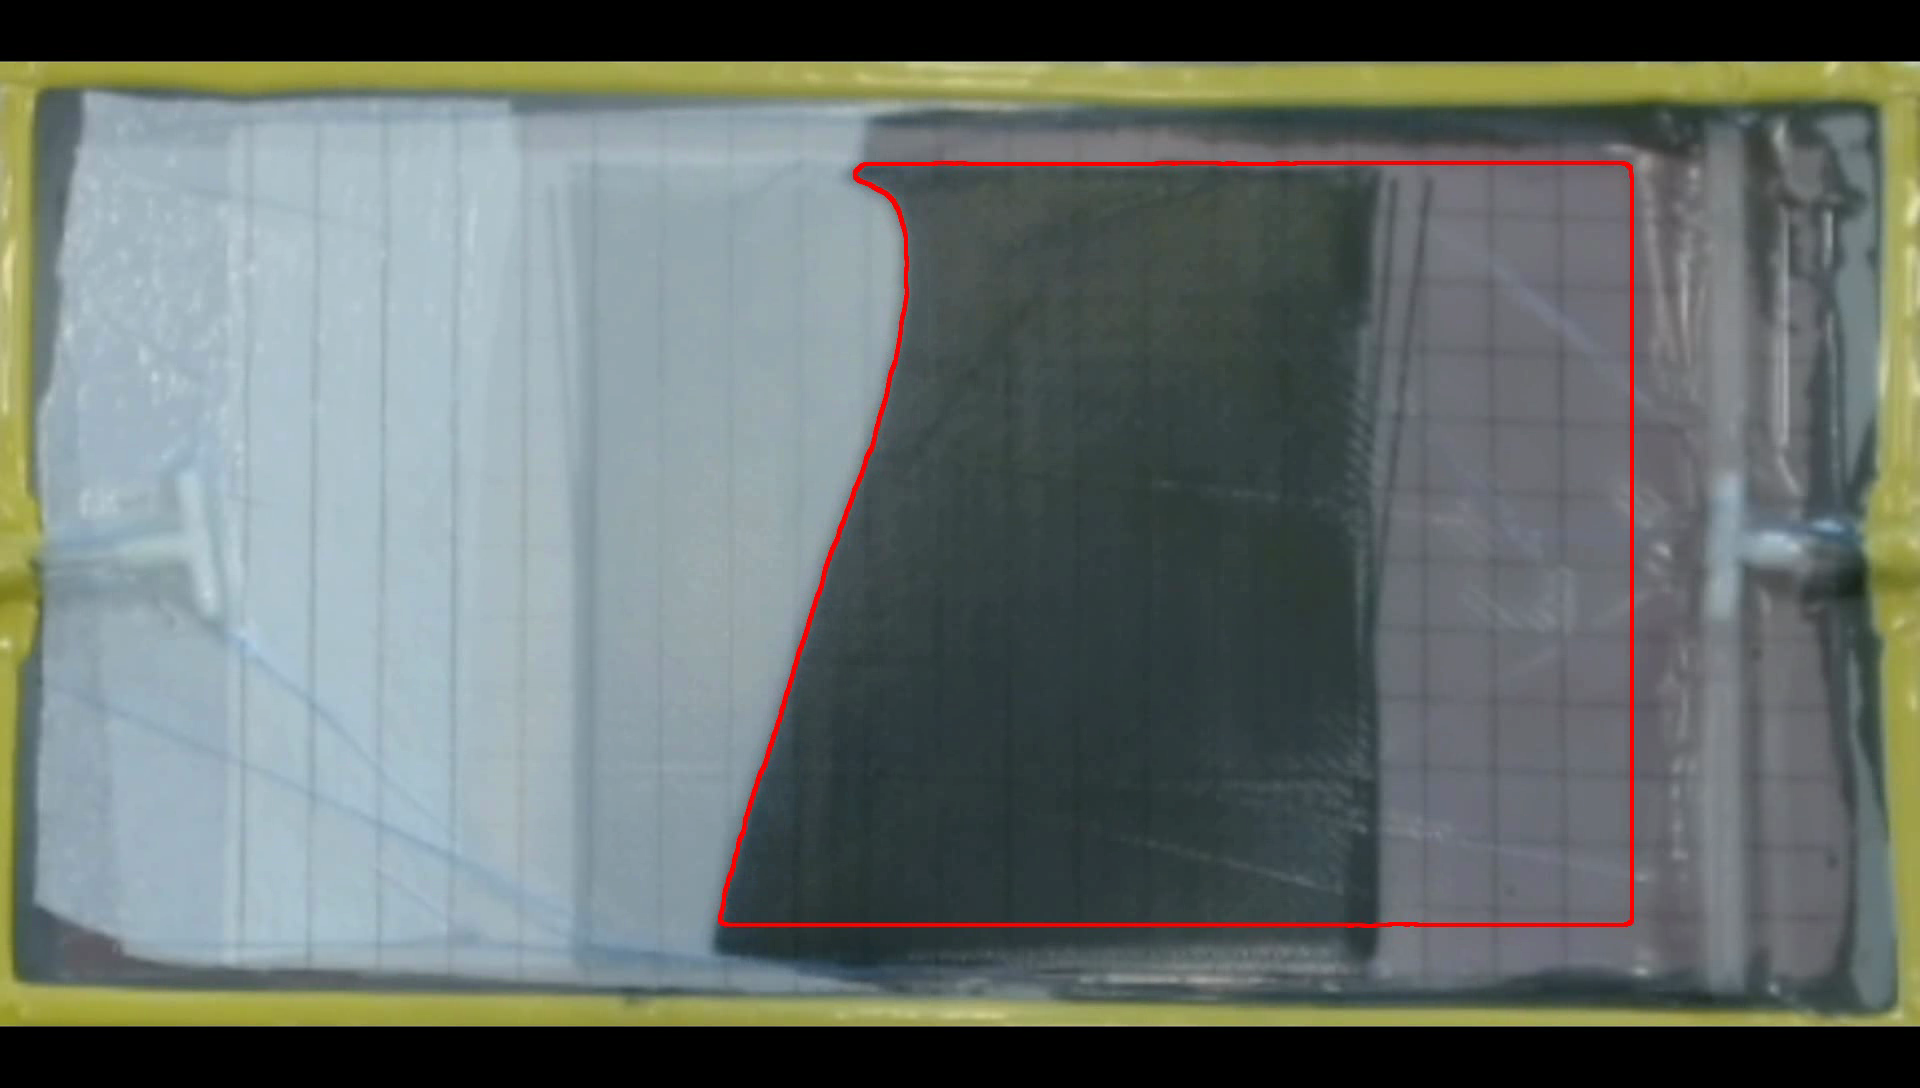
\includegraphics[width=\textwidth]{figures/vrifa_orig_overlay_frame_050.png}
    \caption{Original overlay}
\end{subfigure}
\hfill
\begin{subfigure}[b]{0.32\textwidth}
    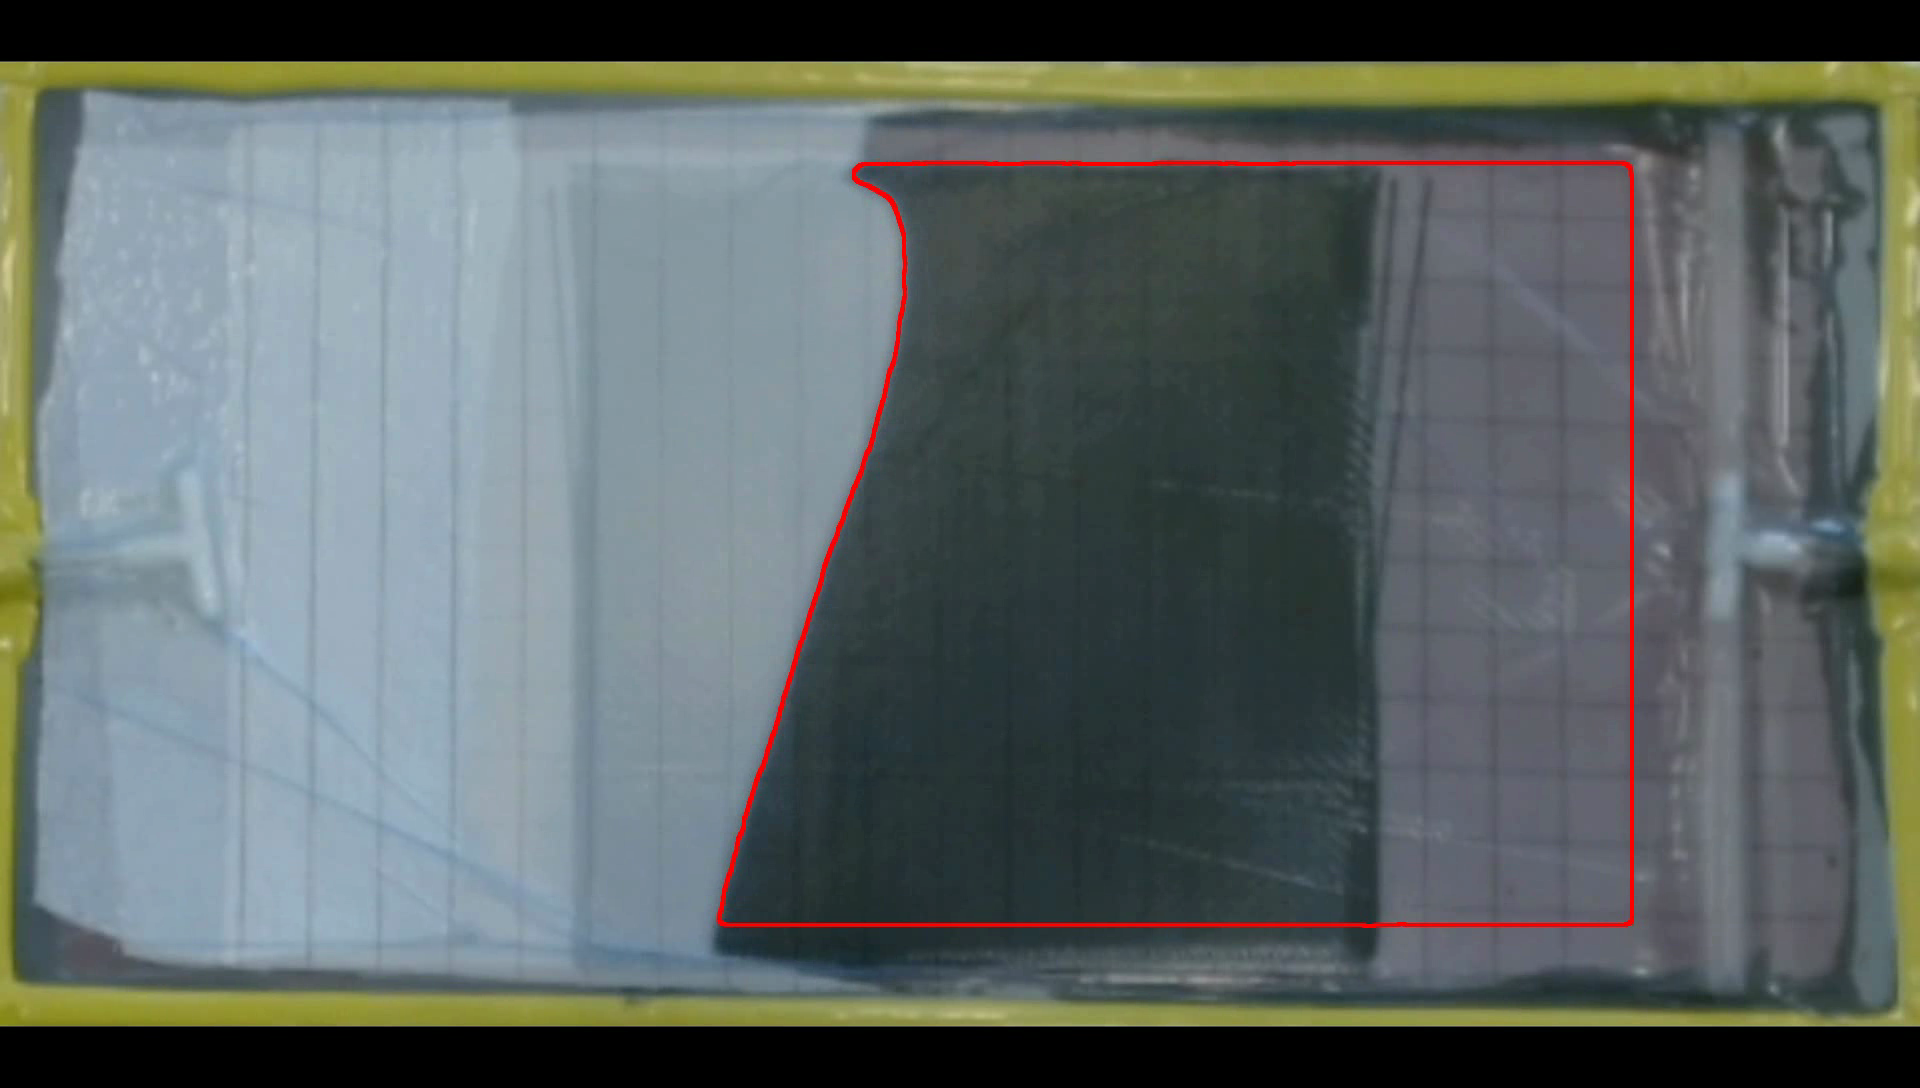
\includegraphics[width=\textwidth]{figures/vrifa_corr_overlay_frame_050.png}
    \caption{Corrected overlay}
\end{subfigure}
\hfill
\begin{subfigure}[b]{0.32\textwidth}
    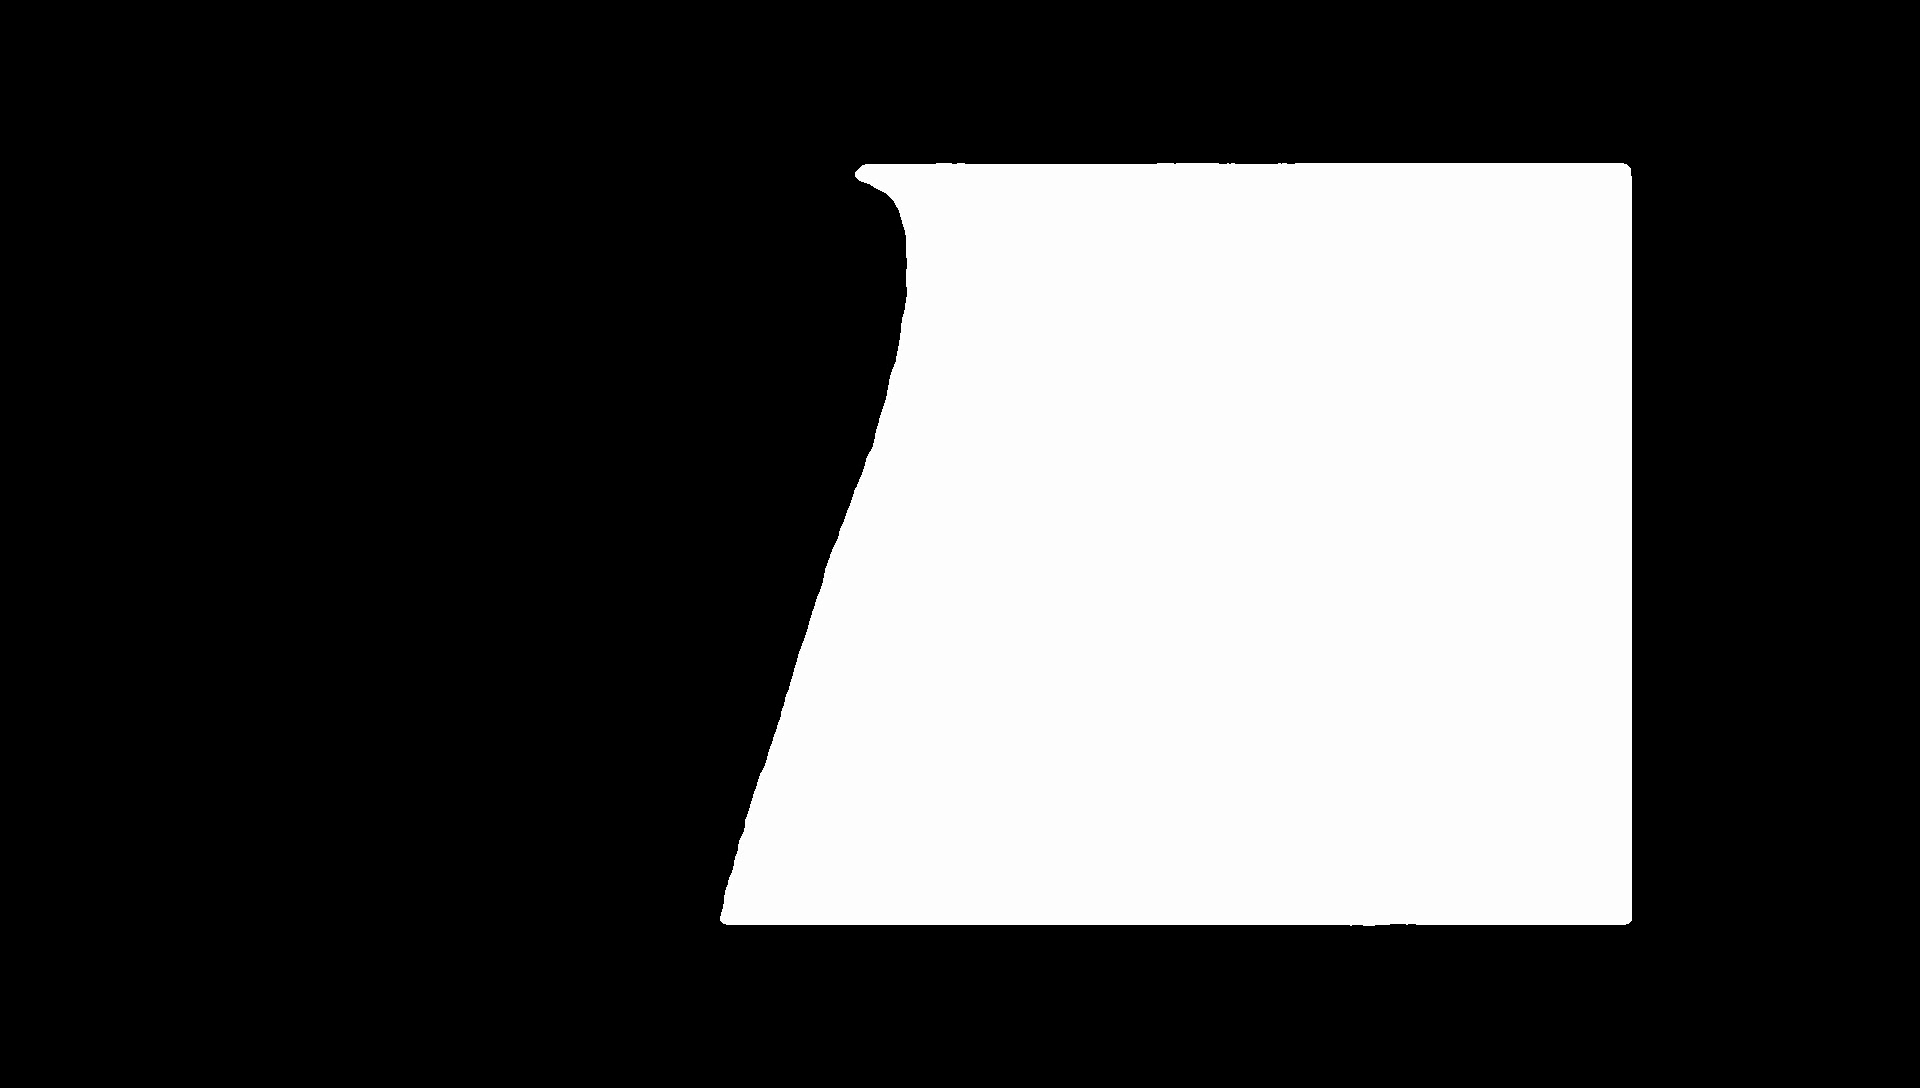
\includegraphics[width=\textwidth]{figures/vrifa_orig_mask_frame_050.png}
    \caption{Original mask}
\end{subfigure}
\caption{VRIFA flow-front detection at frame 50, shortly before exposure event $E_2$. Both original and corrected videos show similar results at this early stage, though subtle differences begin to appear due to the cumulative effect of the $E_1$ correction applied at frame 23.}
\label{fig:vrifa_comparison_50}
\end{figure*}

\begin{figure*}[t]
\centering
\begin{subfigure}[b]{0.32\textwidth}
    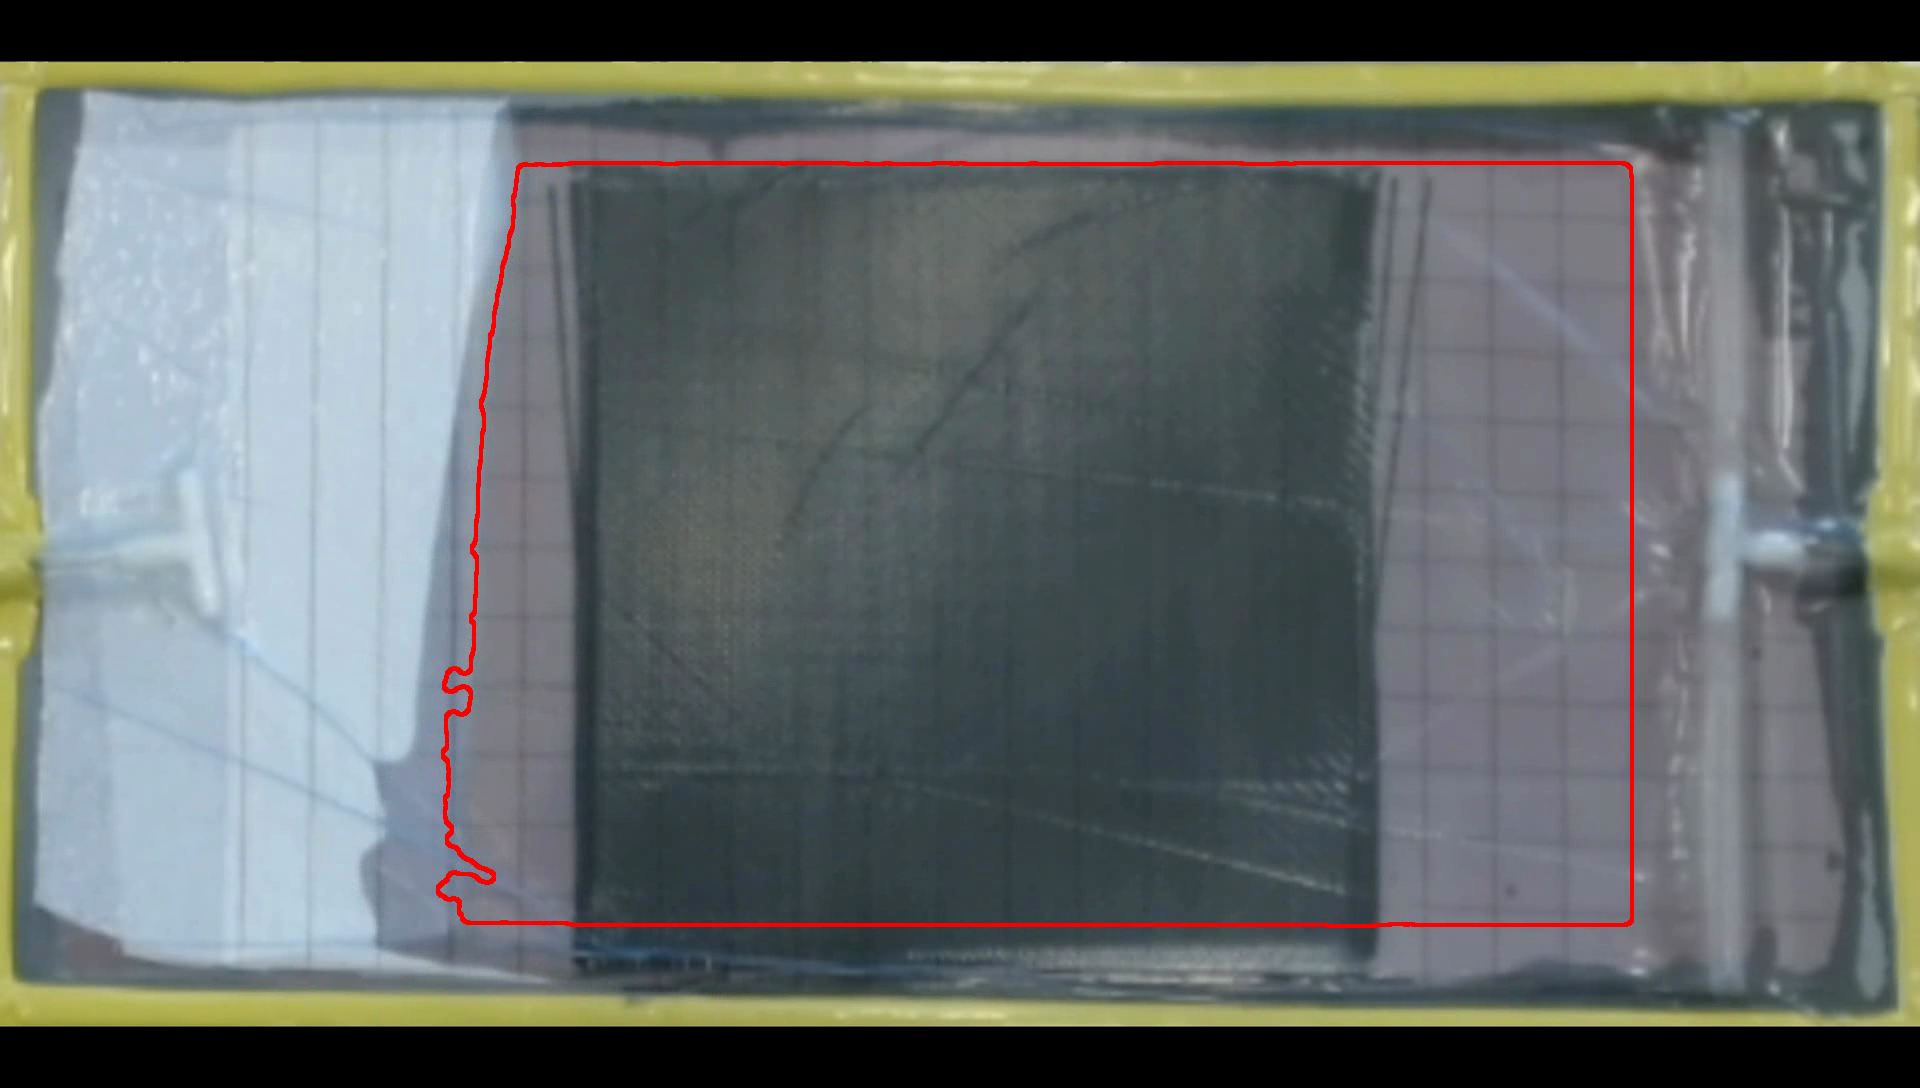
\includegraphics[width=\textwidth]{figures/vrifa_orig_overlay_frame_100.png}
    \caption{Original overlay}
\end{subfigure}
\hfill
\begin{subfigure}[b]{0.32\textwidth}
    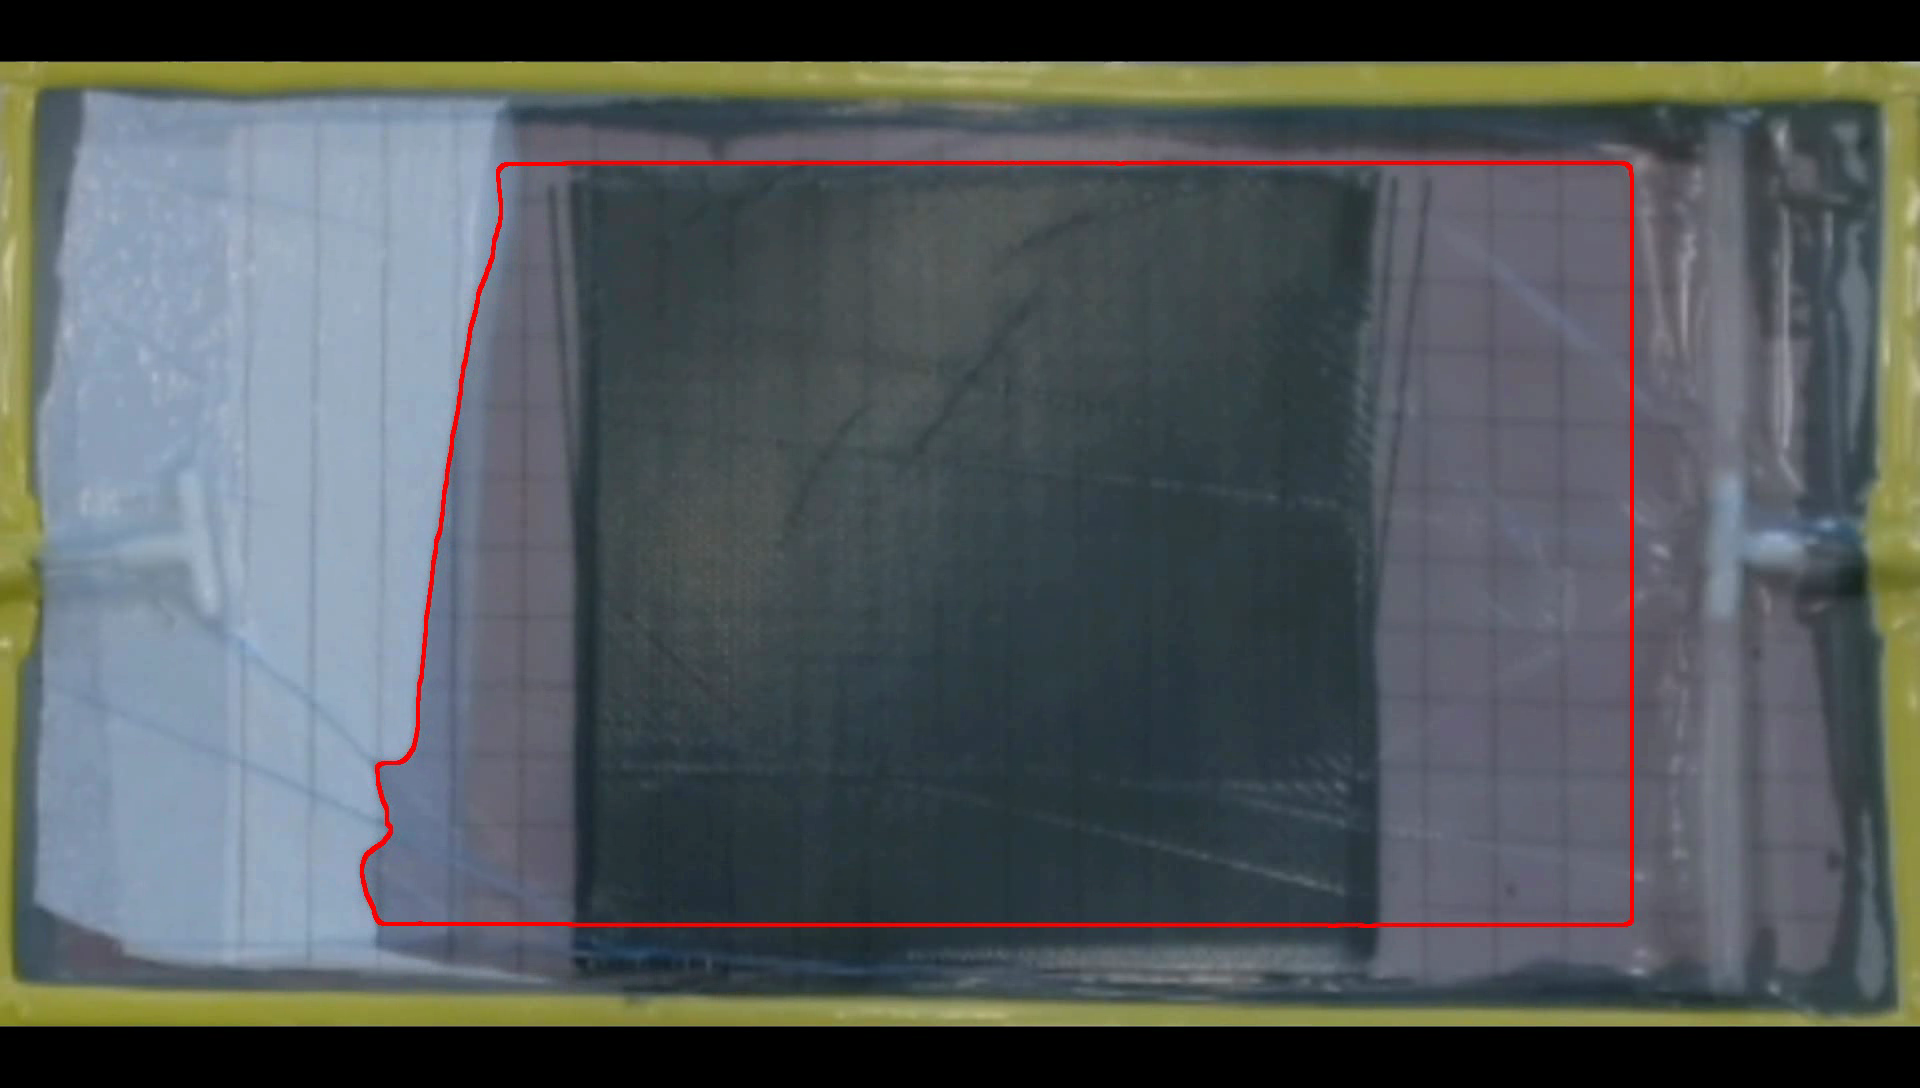
\includegraphics[width=\textwidth]{figures/vrifa_corr_overlay_frame_100.png}
    \caption{Corrected overlay}
\end{subfigure}
\hfill
\begin{subfigure}[b]{0.32\textwidth}
    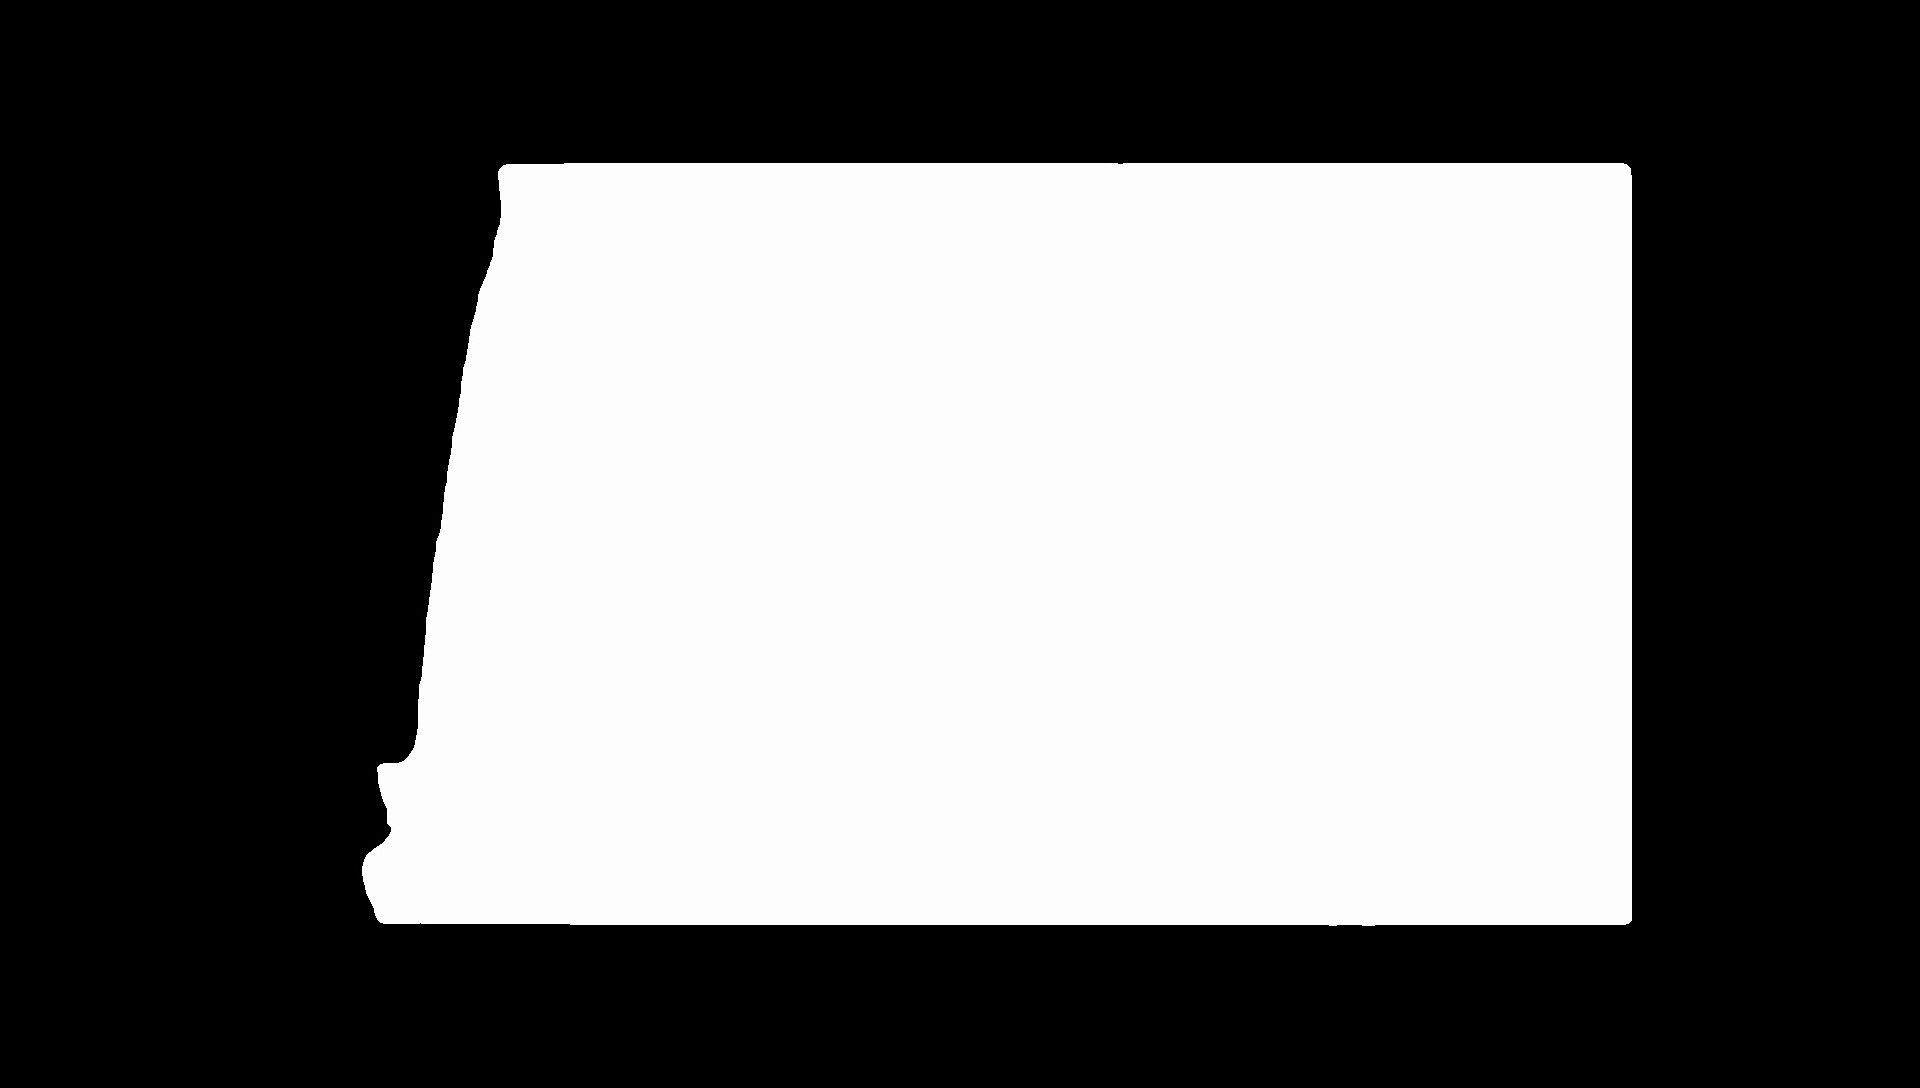
\includegraphics[width=\textwidth]{figures/vrifa_corr_mask_frame_100.png}
    \caption{Corrected mask}
\end{subfigure}
\\[0.5em]
\begin{subfigure}[b]{0.32\textwidth}
    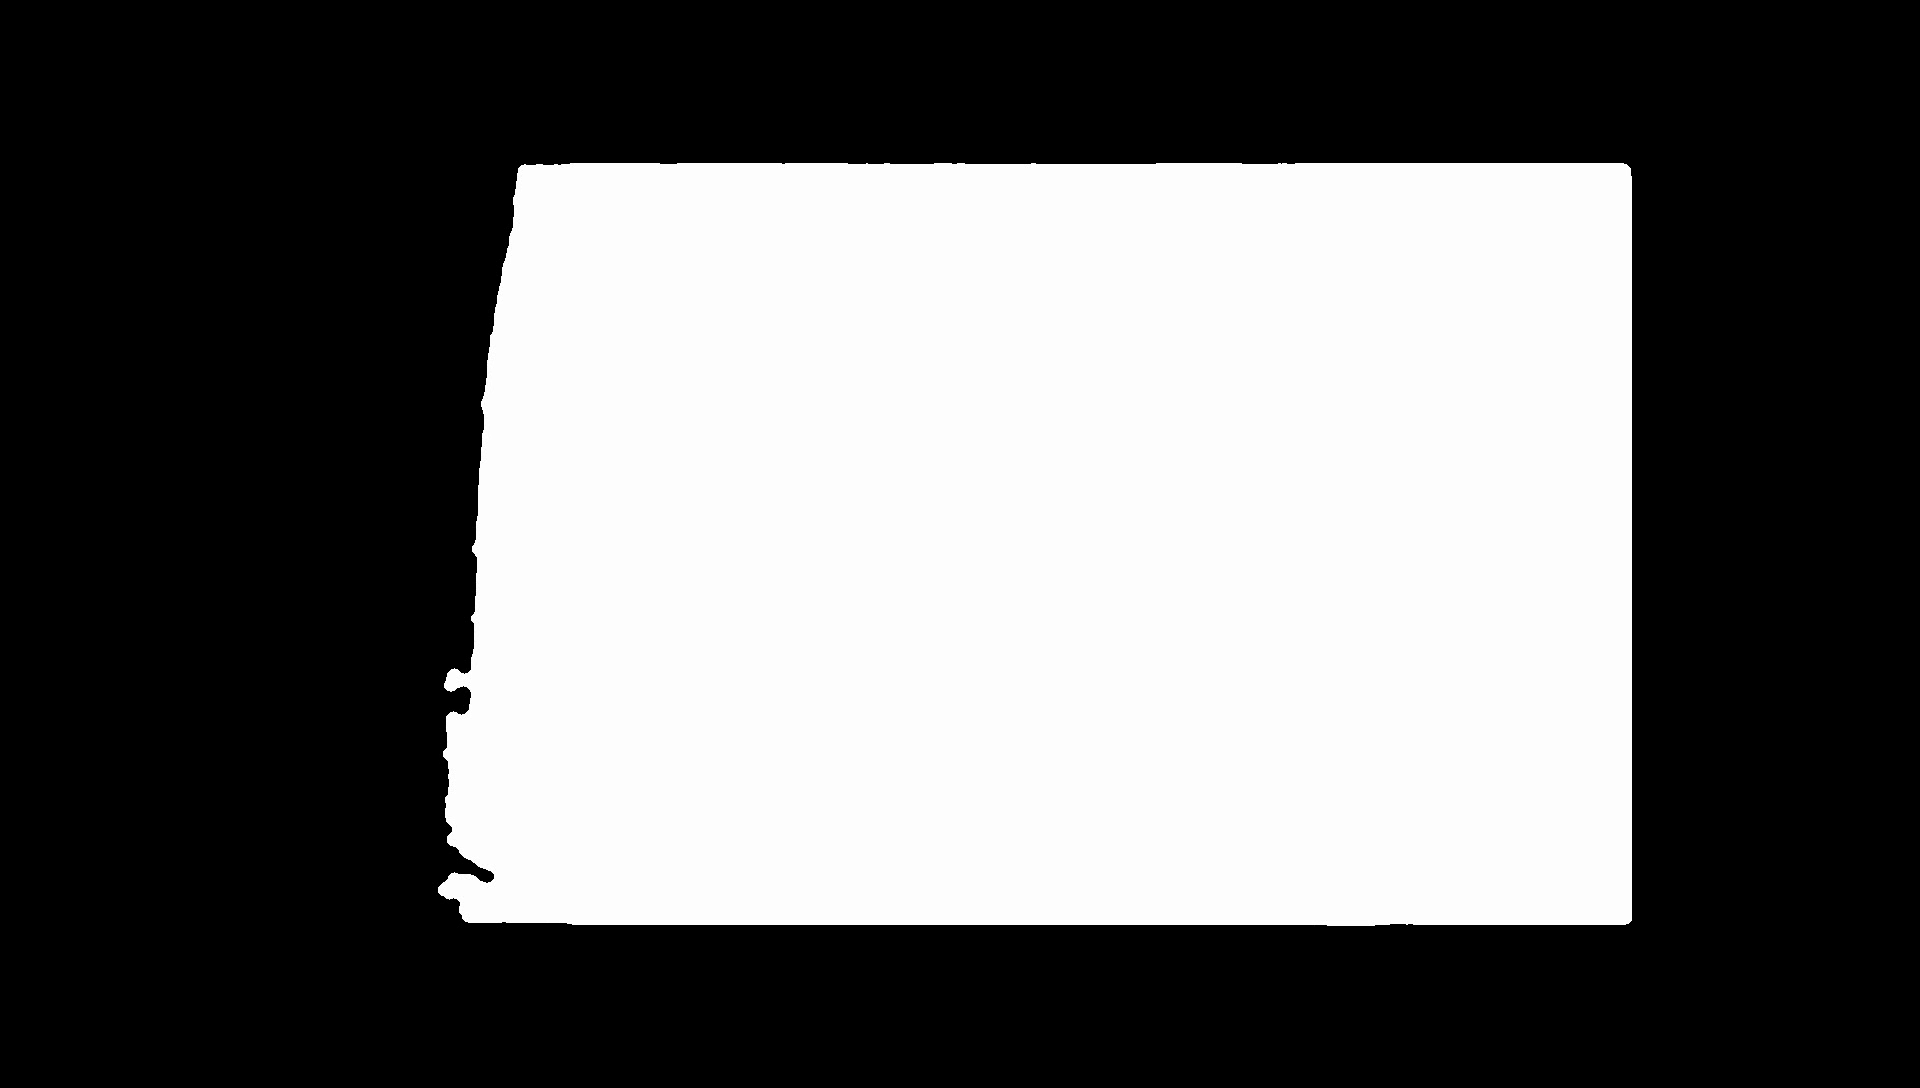
\includegraphics[width=\textwidth]{figures/vrifa_orig_mask_frame_100.png}
    \caption{Original mask}
\end{subfigure}
\hfill
\begin{subfigure}[b]{0.32\textwidth}
    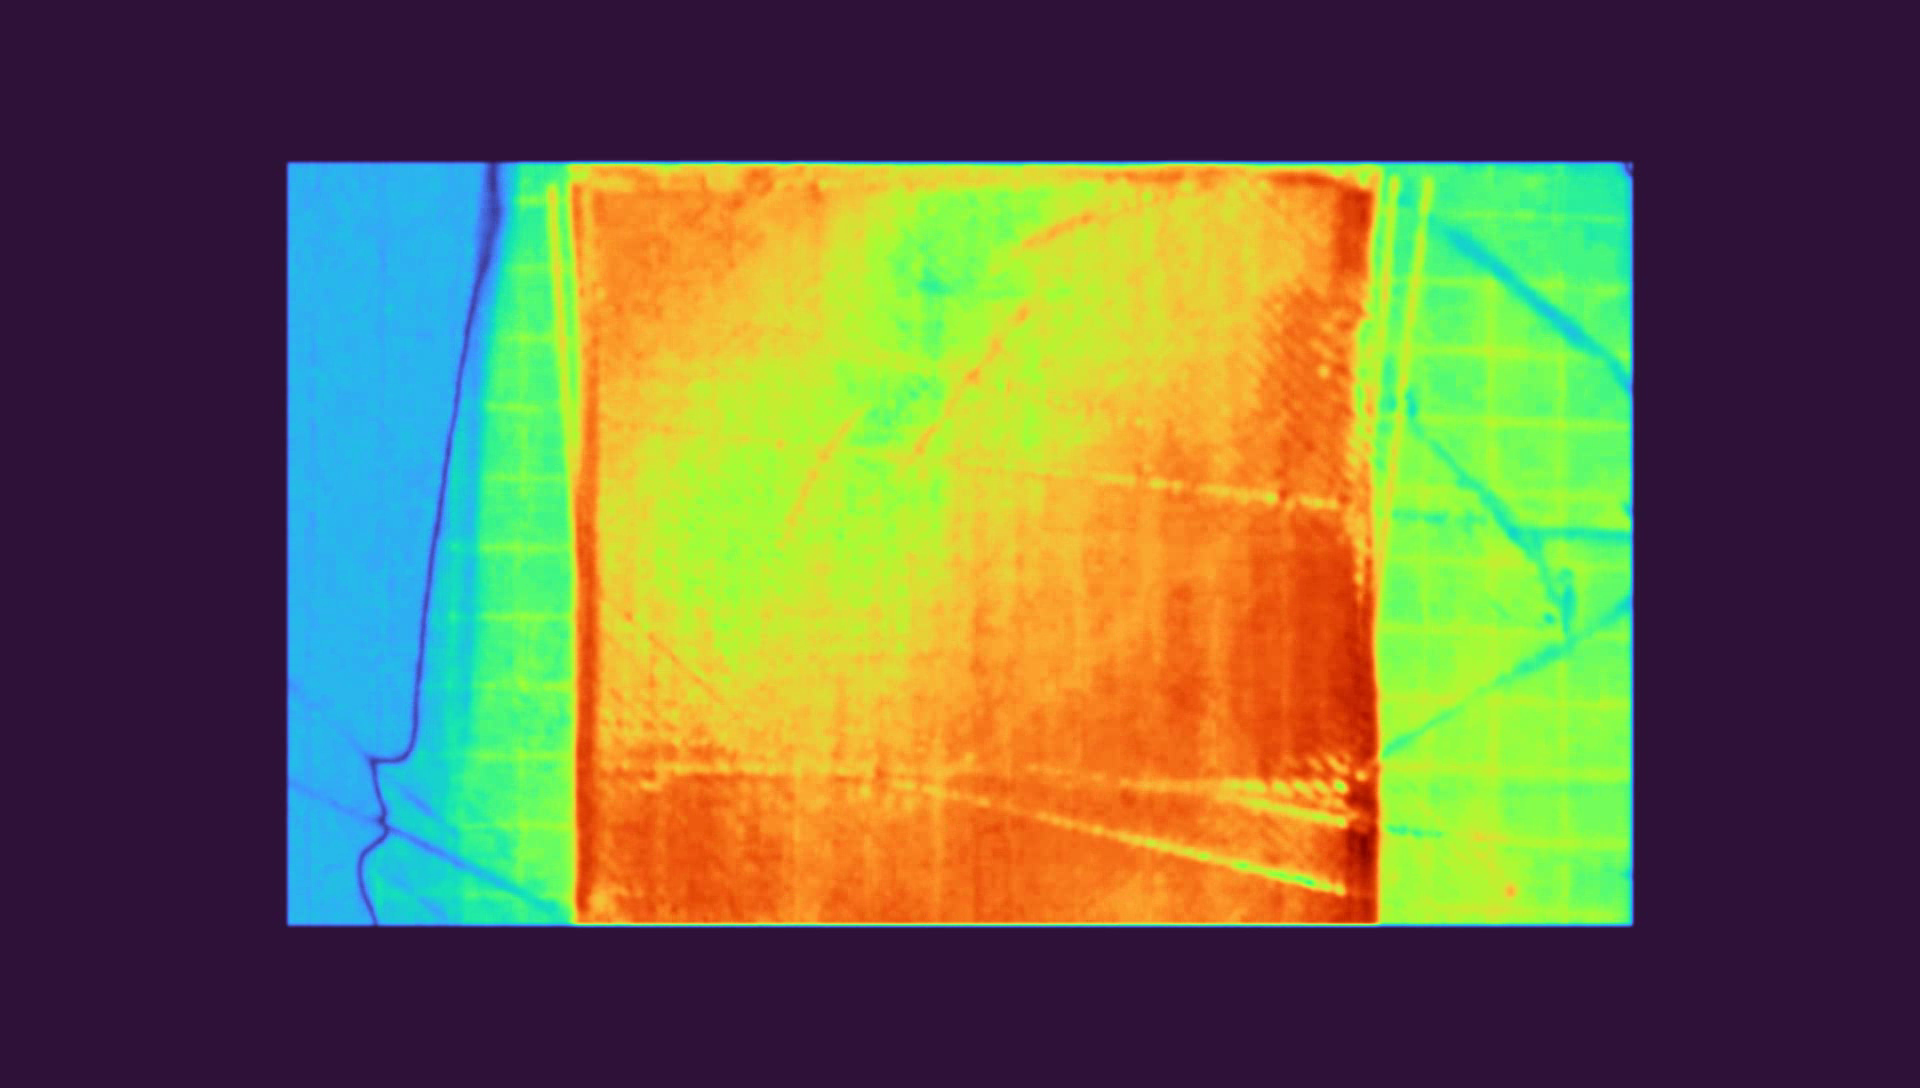
\includegraphics[width=\textwidth]{figures/vrifa_orig_heatmap_frame_100.png}
    \caption{Original heatmap}
\end{subfigure}
\hfill
\begin{subfigure}[b]{0.32\textwidth}
    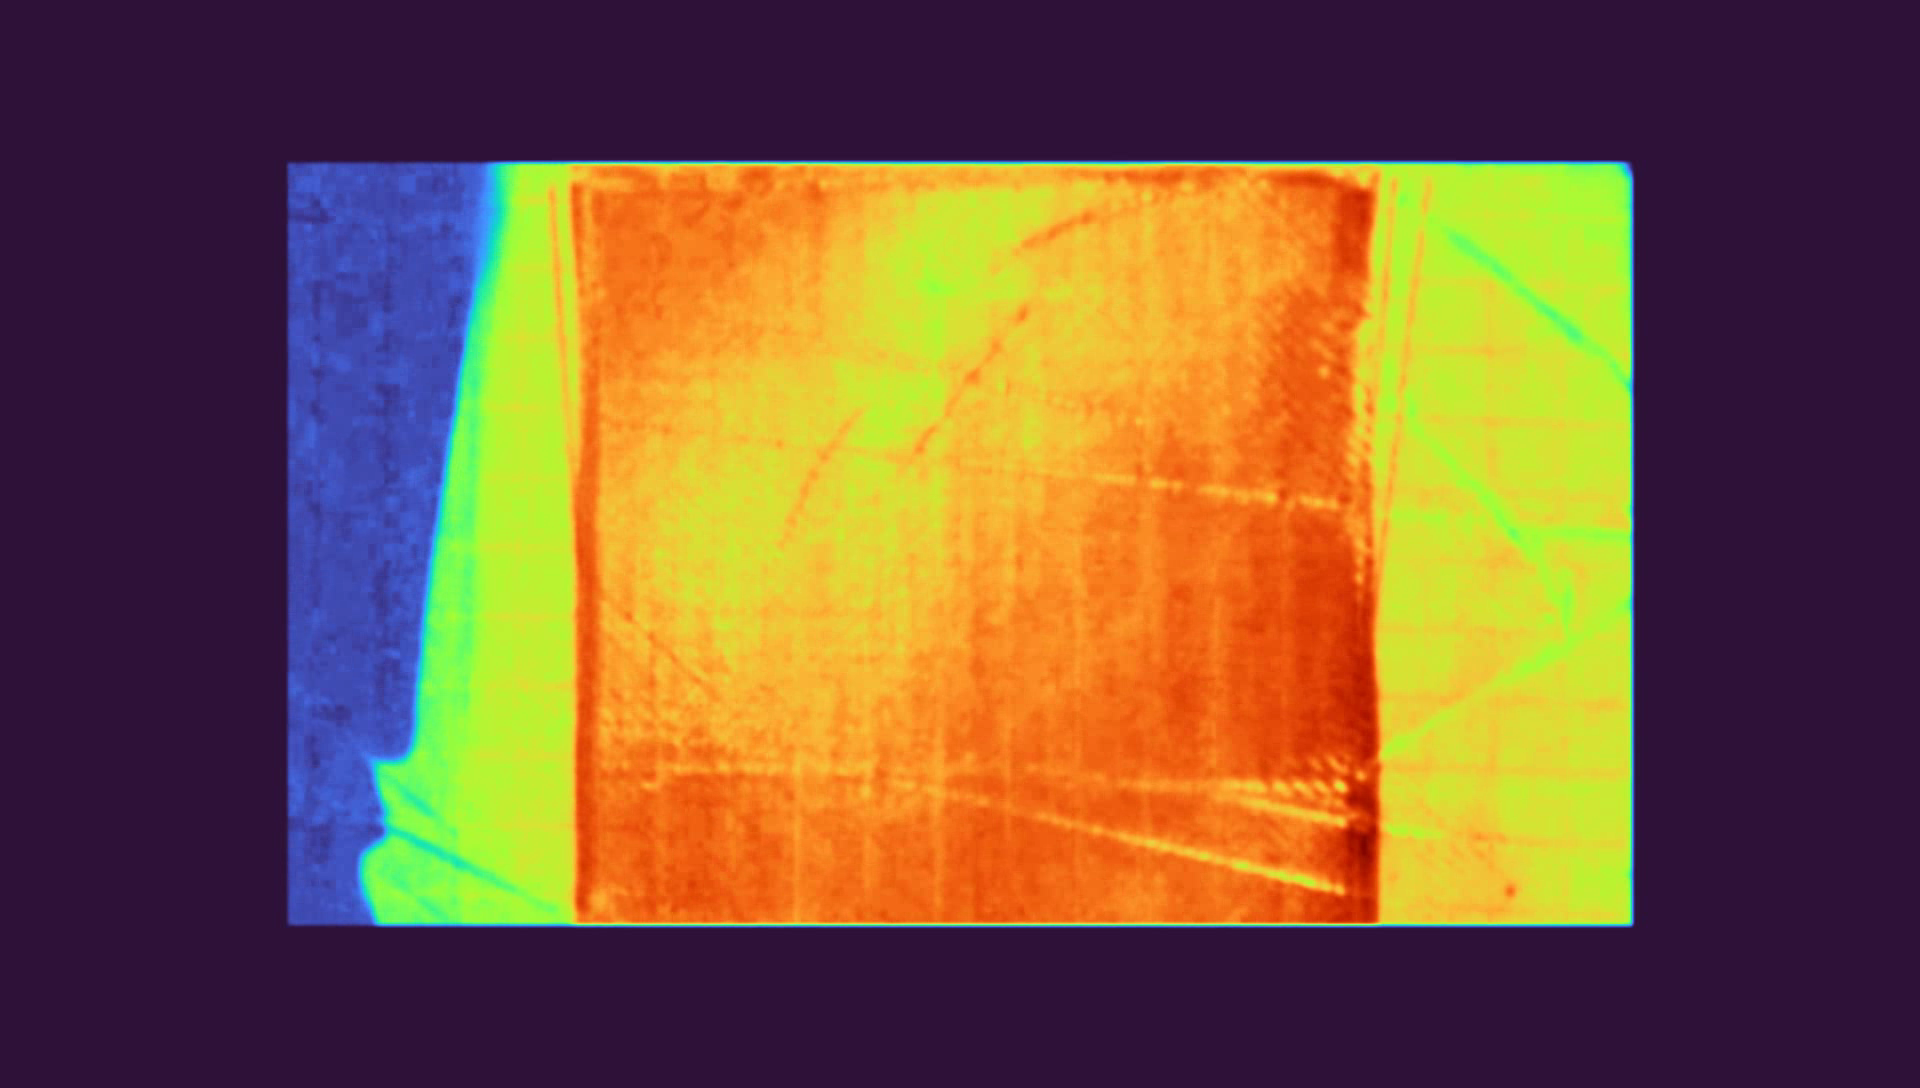
\includegraphics[width=\textwidth]{figures/vrifa_corr_heatmap_frame_100.png}
    \caption{Corrected heatmap}
\end{subfigure}
\caption{VRIFA flow-front detection at frame 100. The corrected video produces cleaner segmentation with fewer spurious detections. The heatmap shows cumulative flow-front progression with color indicating detection time.}
\label{fig:vrifa_comparison}
\end{figure*}

\begin{figure*}[t]
\centering
\begin{subfigure}[b]{0.32\textwidth}
    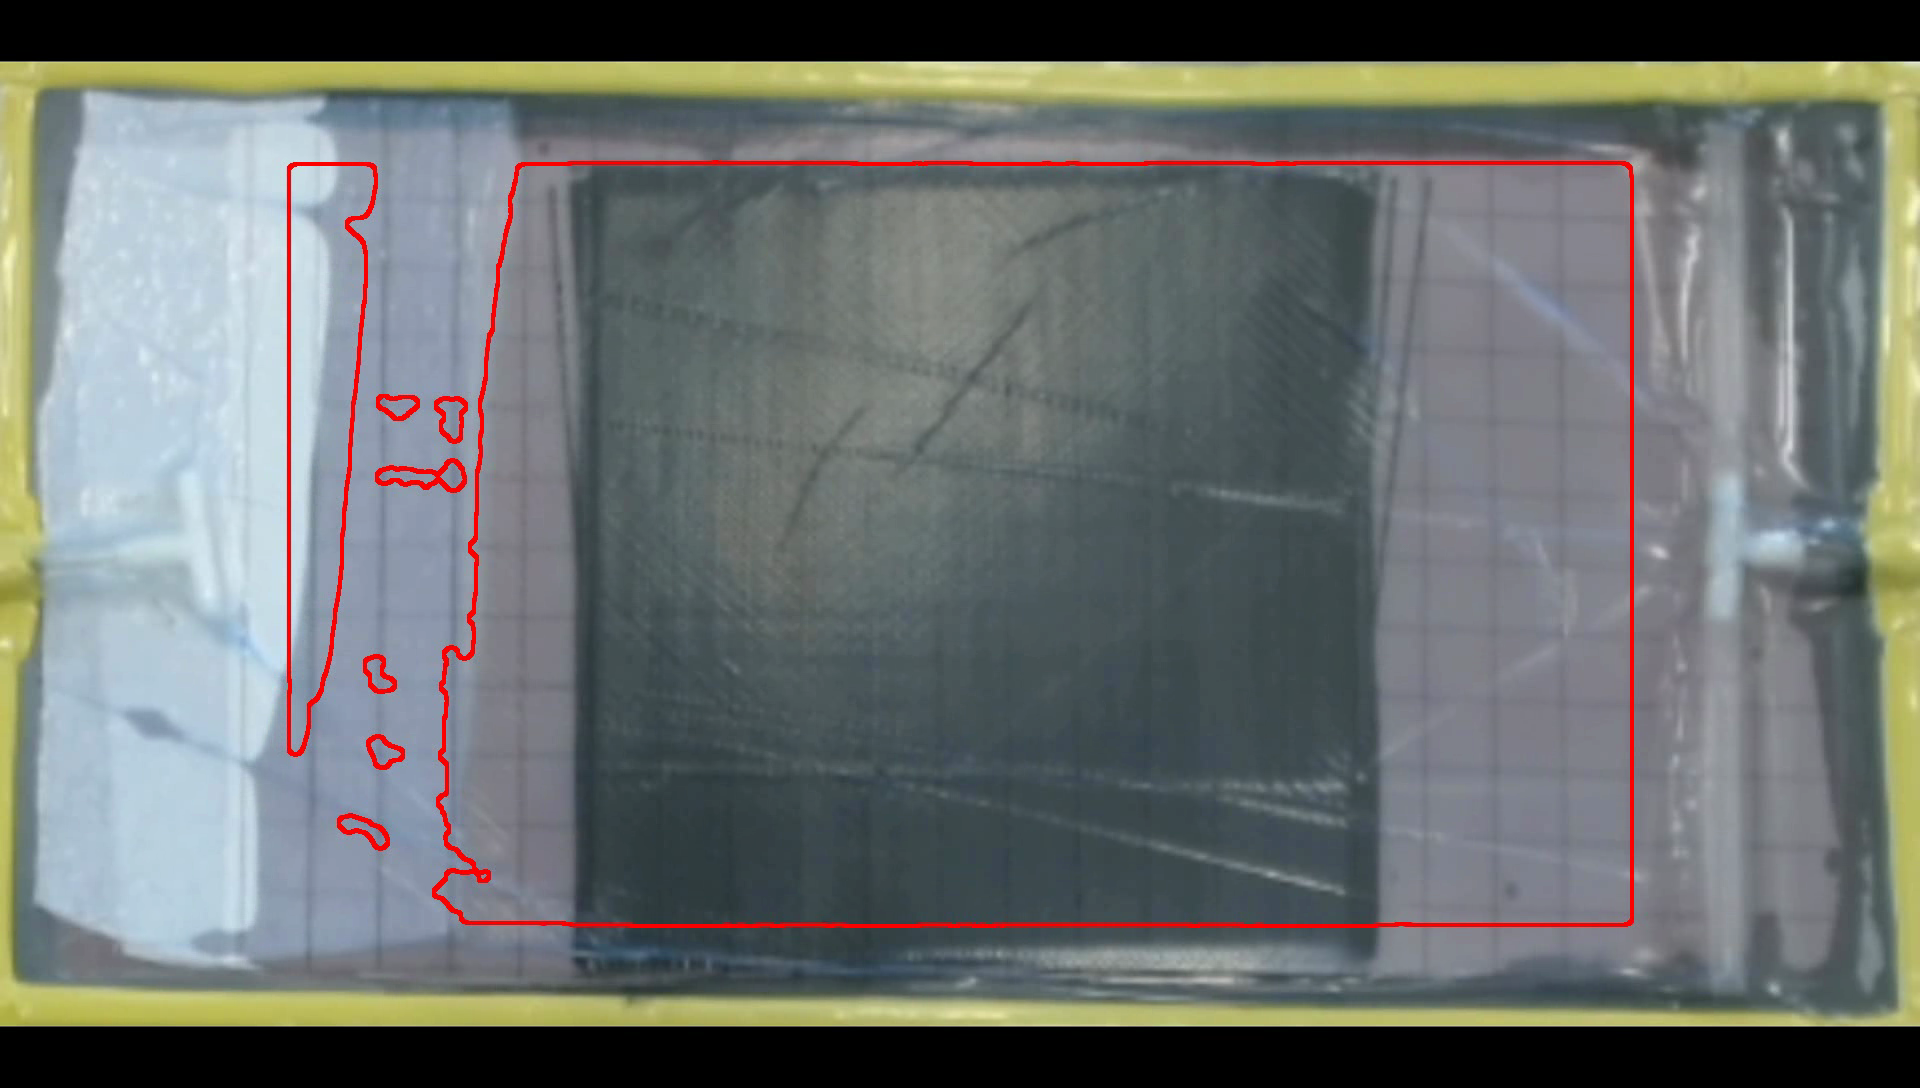
\includegraphics[width=\textwidth]{figures/vrifa_orig_overlay_frame_150.png}
    \caption{Original overlay}
\end{subfigure}
\hfill
\begin{subfigure}[b]{0.32\textwidth}
    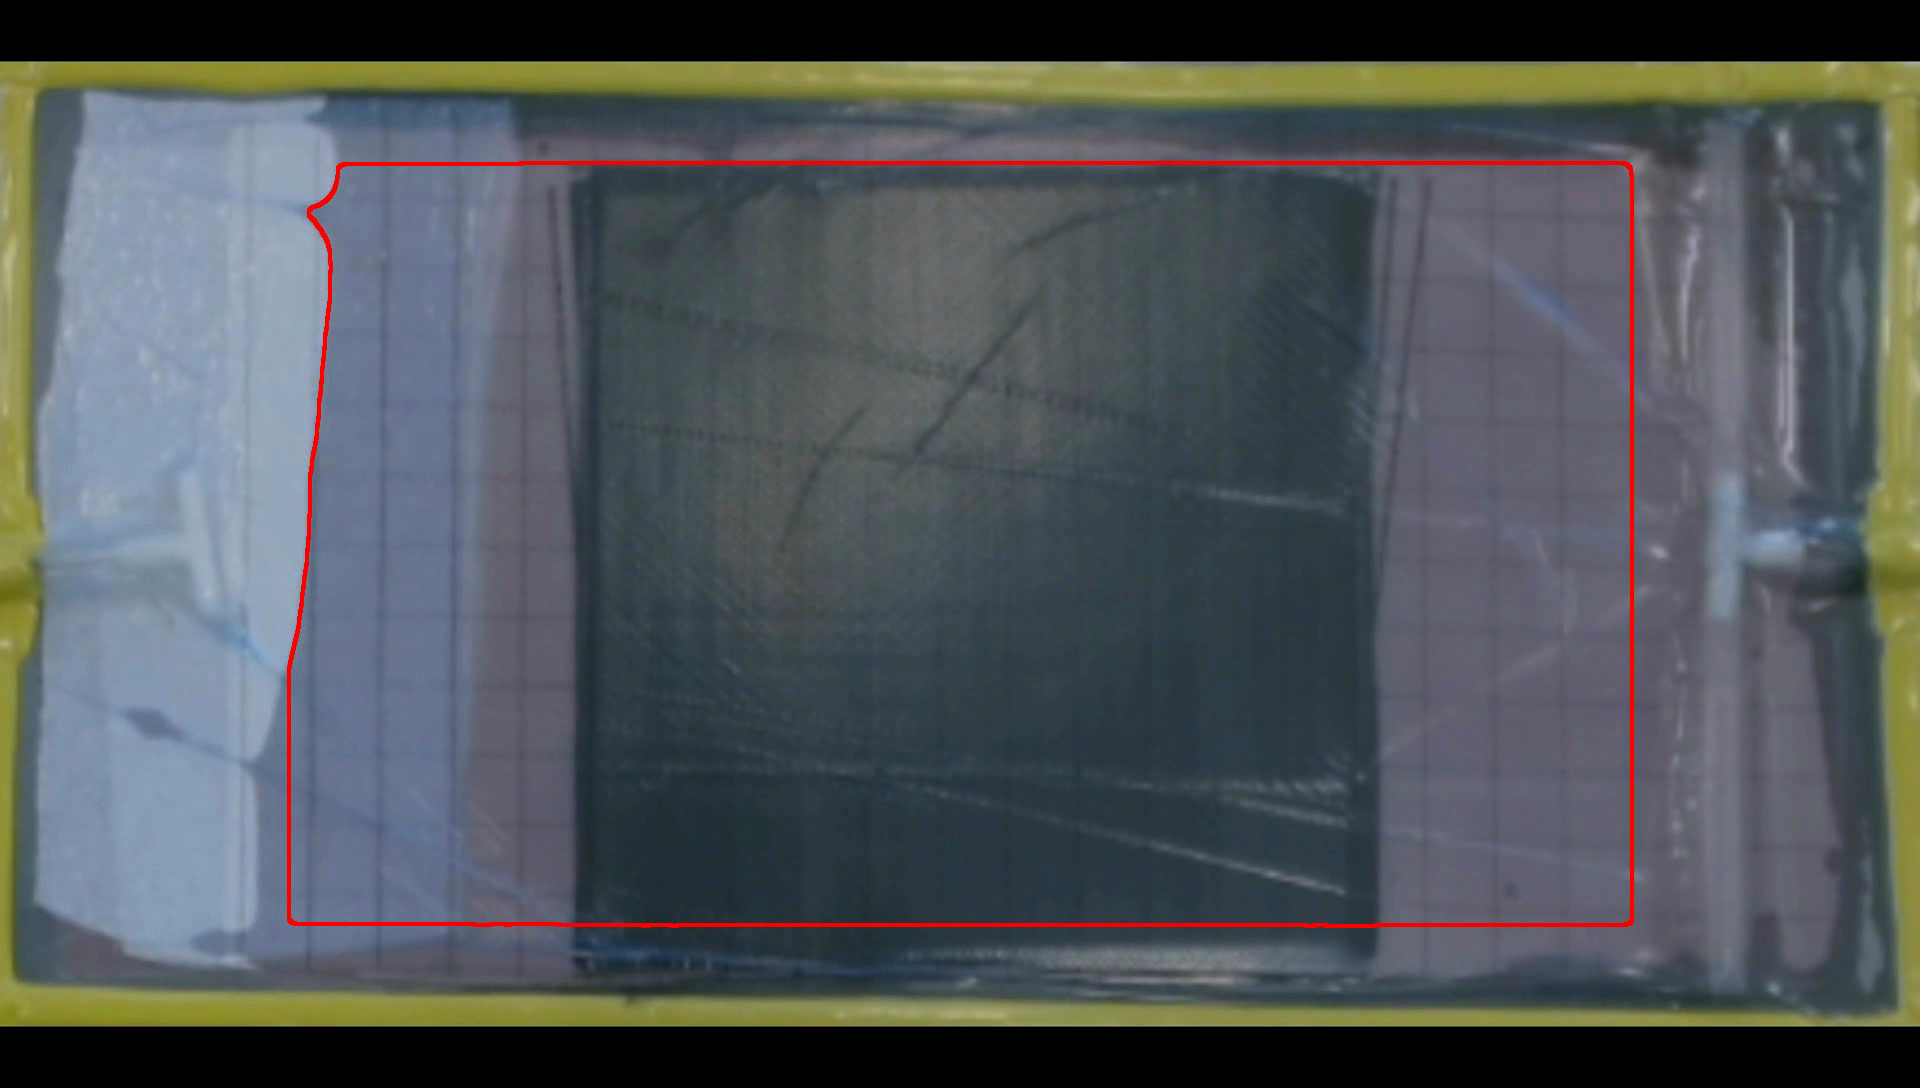
\includegraphics[width=\textwidth]{figures/vrifa_corr_overlay_frame_150.png}
    \caption{Corrected overlay}
\end{subfigure}
\hfill
\begin{subfigure}[b]{0.32\textwidth}
    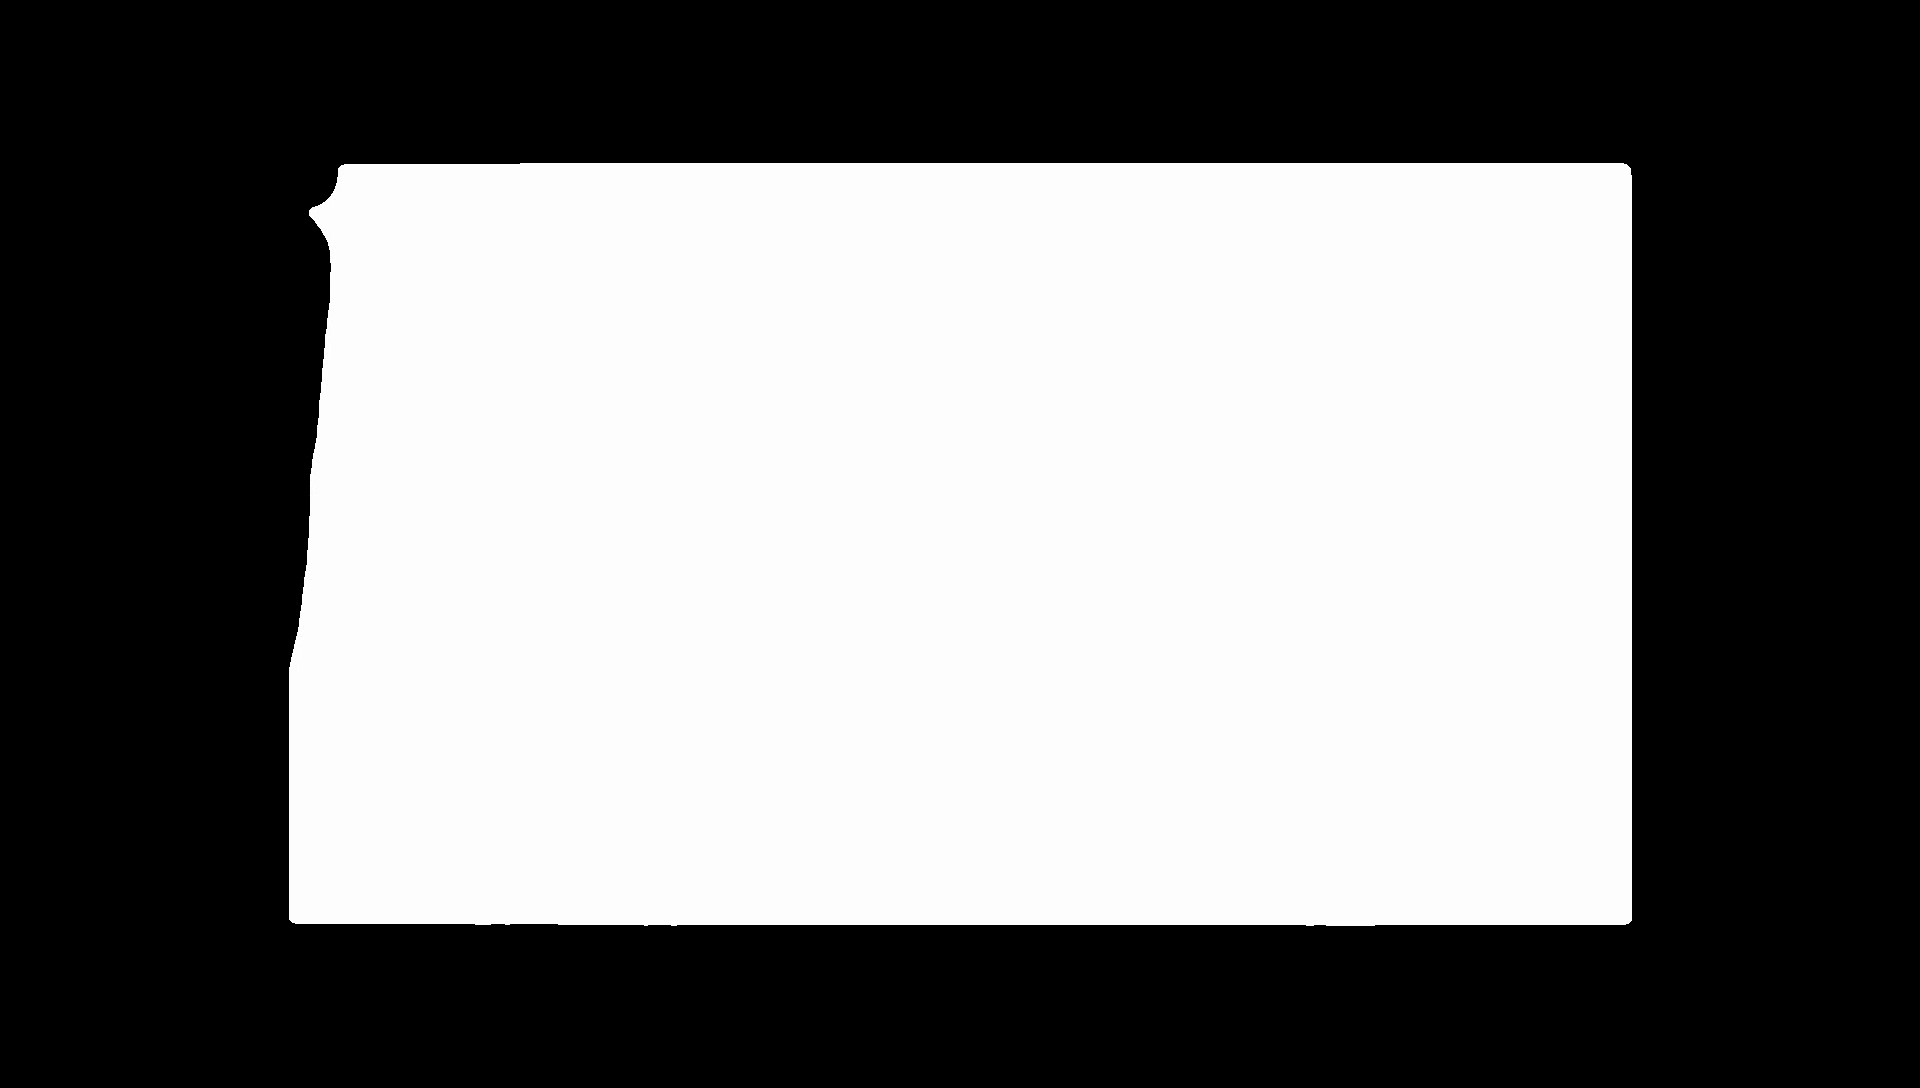
\includegraphics[width=\textwidth]{figures/vrifa_corr_mask_frame_150.png}
    \caption{Corrected mask}
\end{subfigure}
\\[0.5em]
\begin{subfigure}[b]{0.32\textwidth}
    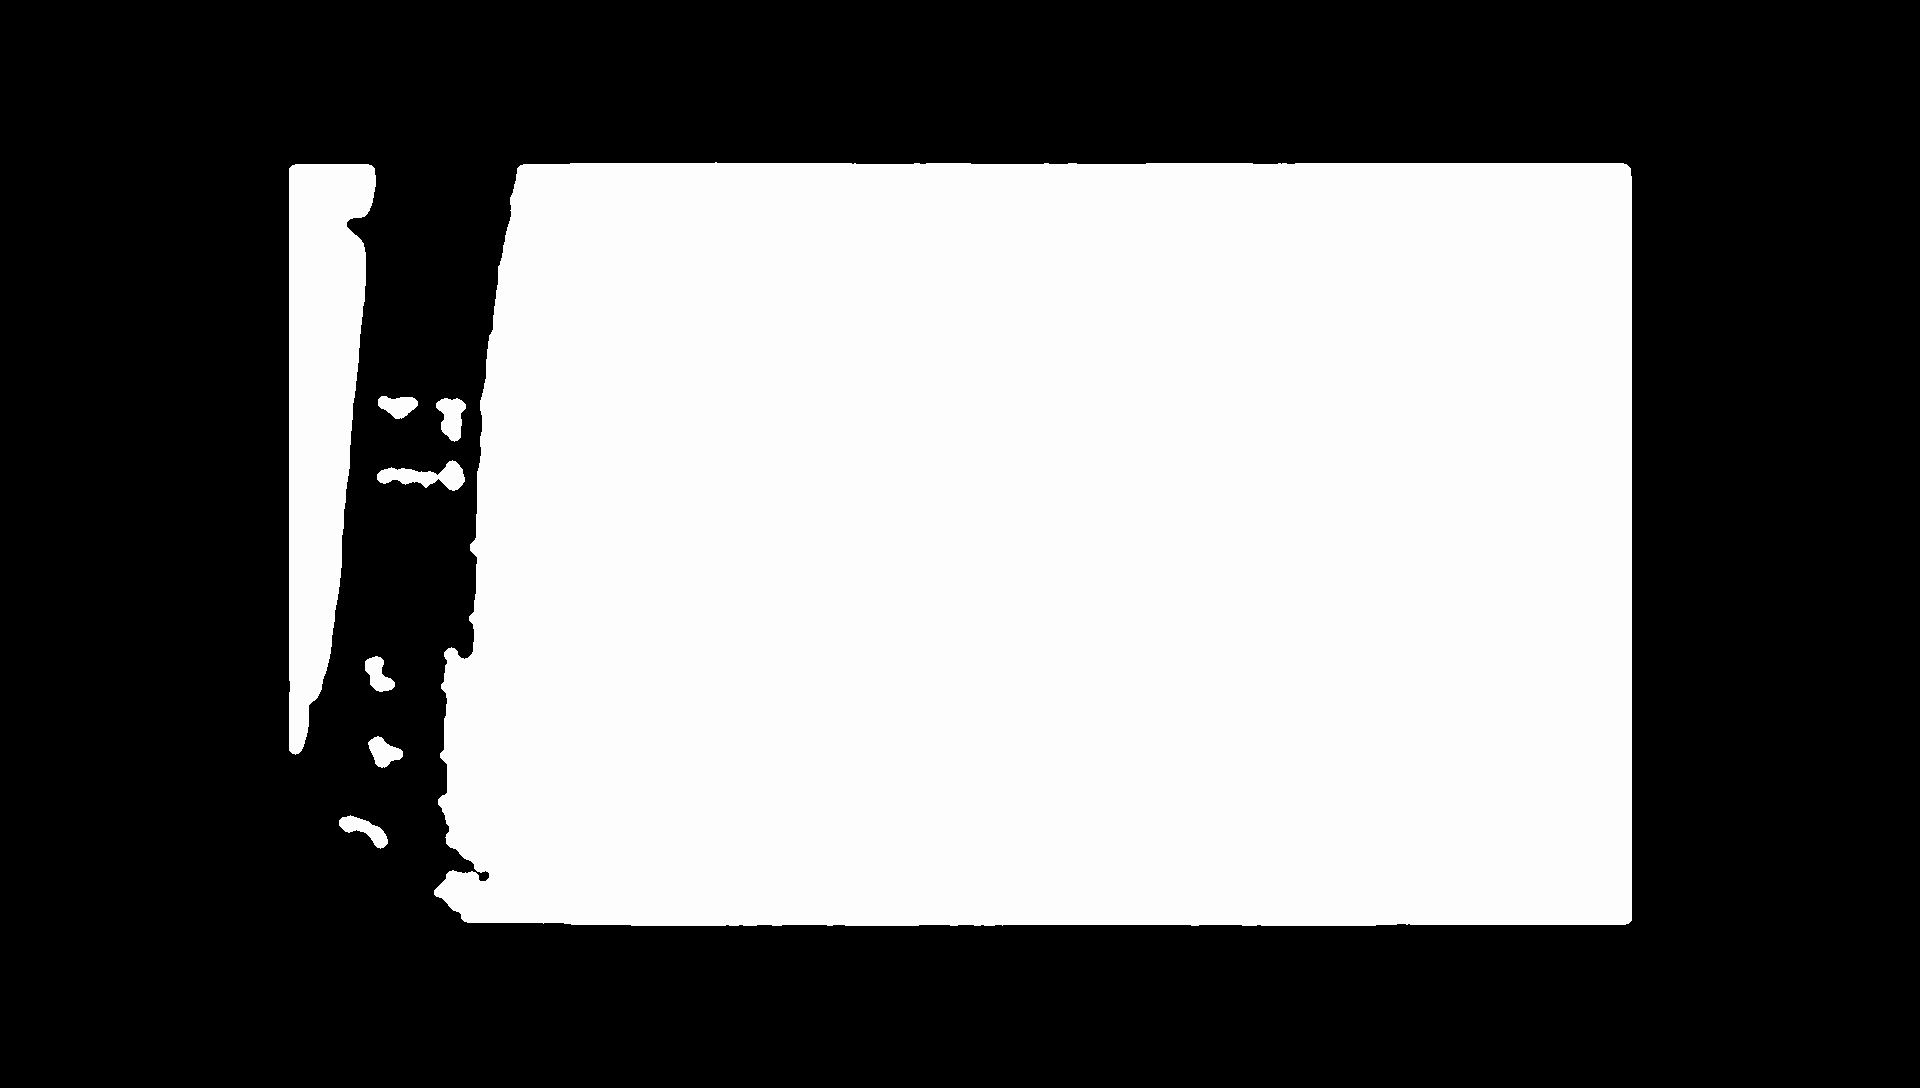
\includegraphics[width=\textwidth]{figures/vrifa_orig_mask_frame_150.png}
    \caption{Original mask}
\end{subfigure}
\hfill
\begin{subfigure}[b]{0.32\textwidth}
    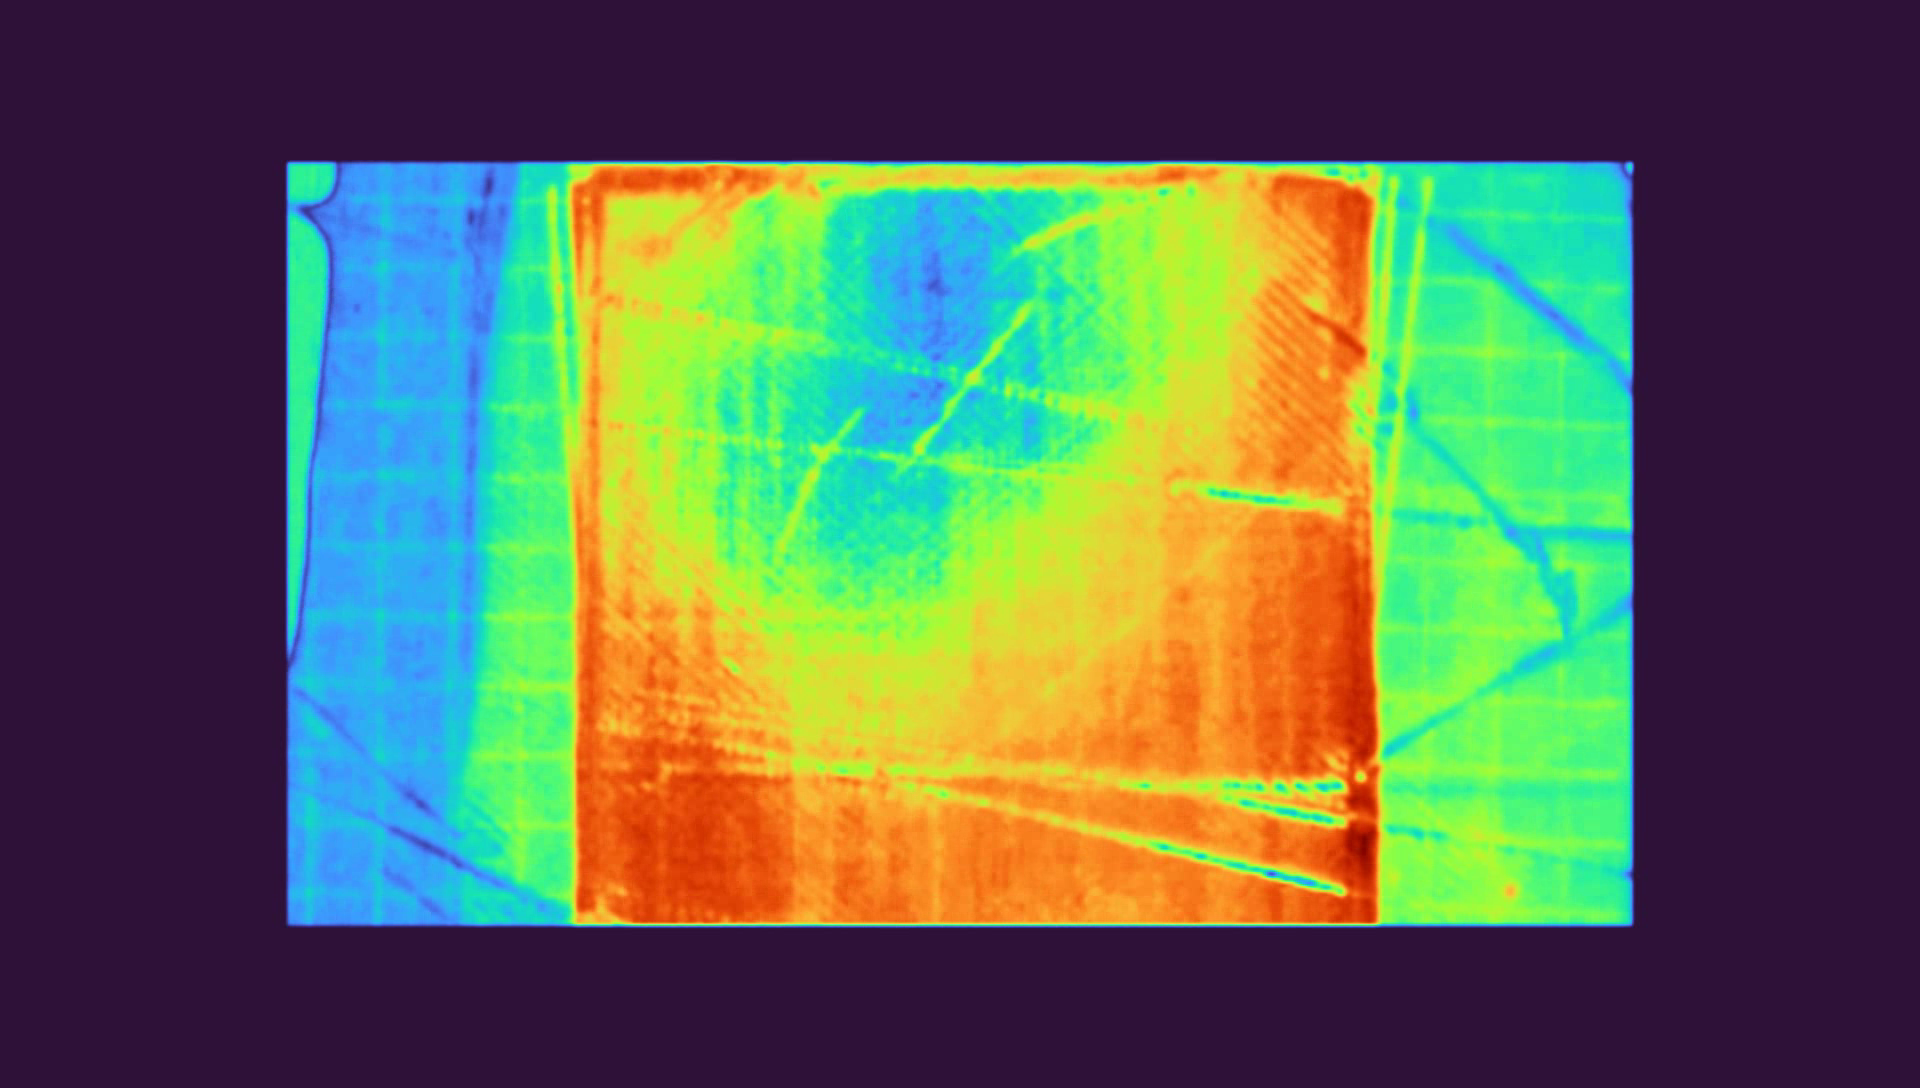
\includegraphics[width=\textwidth]{figures/vrifa_orig_heatmap_frame_150.png}
    \caption{Original heatmap}
\end{subfigure}
\hfill
\begin{subfigure}[b]{0.32\textwidth}
    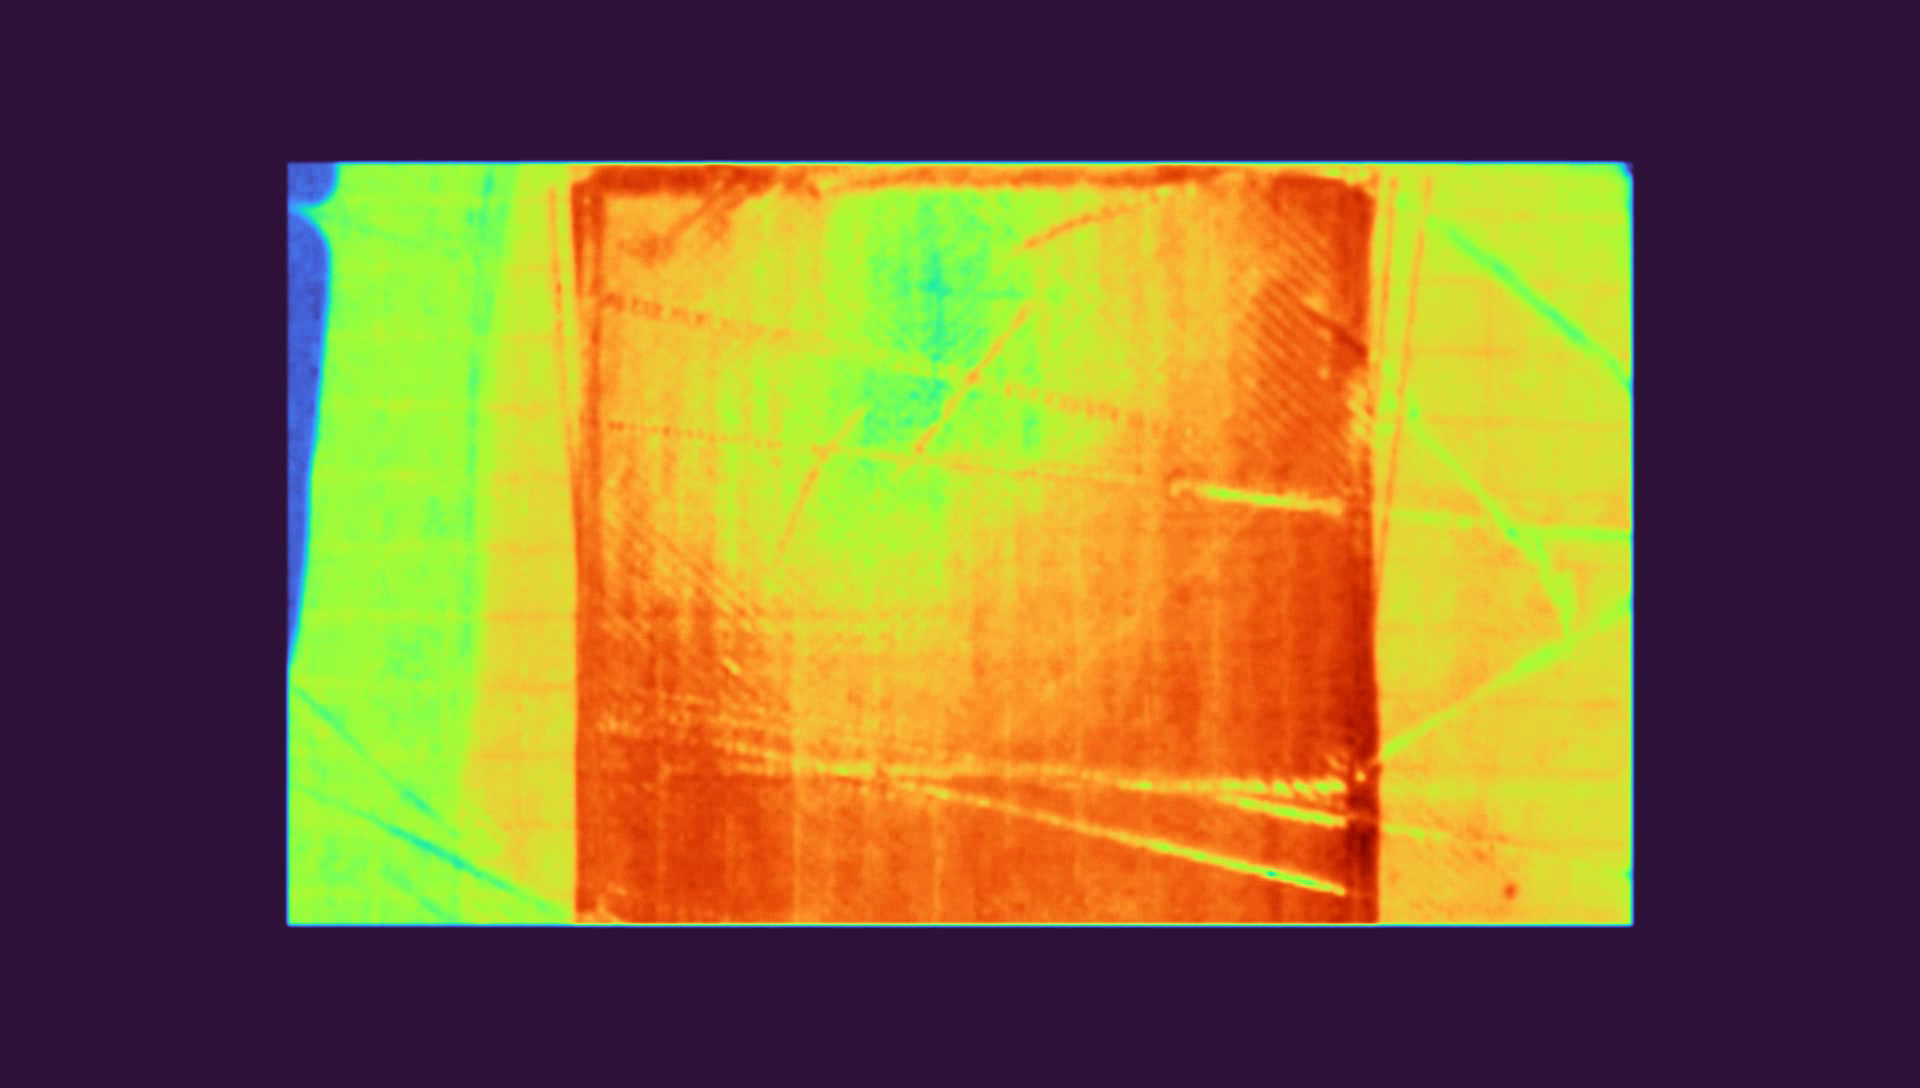
\includegraphics[width=\textwidth]{figures/vrifa_corr_heatmap_frame_150.png}
    \caption{Corrected heatmap}
\end{subfigure}
\caption{VRIFA outputs at frame 150 after all three exposure events. The original video's heatmap shows discontinuities corresponding to exposure artifacts, while the corrected video produces smoother contours without exposure-induced artifacts. The difference is most visible in edge regions where exposure changes created false positive detections.}
\label{fig:vrifa_heatmap}
\end{figure*}

Table~\ref{tab:vrifa_comparison} quantifies the improvement.

\begin{table}[t]
\centering
\caption{VRIFA processing comparison.}
\label{tab:vrifa_comparison}
\begin{tabular}{lcc}
\toprule
\textbf{Metric} & \textbf{Original} & \textbf{Corrected} \\
\midrule
Final wet area (px) & 524,891 & 521,743 \\
Mean area change/frame & 2,893 & 2,614 \\
Std of area change & 487 & 312 \\
Max area jump & 4,217 & 1,893 \\
\bottomrule
\end{tabular}
\end{table}

Maximum area jump reduced by 55\% and variance reduced by 36\%.

\begin{figure}[t]
\centering
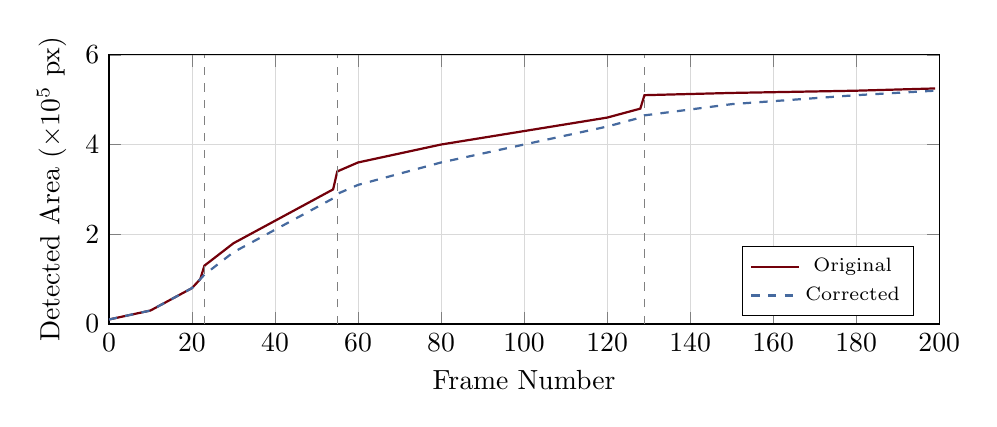
\begin{tikzpicture}
    \begin{axis}[
        width=\columnwidth,
        height=5cm,
        xlabel={Frame Number},
        ylabel={Detected Area ($\times 10^5$ px)},
        xmin=0, xmax=200,
        ymin=0, ymax=6,
        grid=both,
        grid style={line width=0.1pt, draw=gray!30},
        legend pos=south east,
        legend style={font=\scriptsize},
    ]
    \addplot[color=garnet, thick, mark=none] coordinates {
        (0,0.1) (10,0.3) (20,0.8) (22,1.0) (23,1.3) (30,1.8) (40,2.3) (50,2.8) (54,3.0) (55,3.4) (60,3.6) (80,4.0) (100,4.3) (120,4.6) (128,4.8) (129,5.1) (150,5.15) (180,5.2) (199,5.25)
    };
    \addlegendentry{Original}
    \addplot[color=atlantic, thick, mark=none, dashed] coordinates {
        (0,0.1) (10,0.3) (20,0.8) (22,1.0) (23,1.1) (30,1.6) (40,2.1) (50,2.6) (54,2.8) (55,2.9) (60,3.1) (80,3.6) (100,4.0) (120,4.4) (128,4.6) (129,4.65) (150,4.9) (180,5.1) (199,5.2)
    };
    \addlegendentry{Corrected}
    \draw[gray, thin, dashed] (axis cs:23,0) -- (axis cs:23,6);
    \draw[gray, thin, dashed] (axis cs:55,0) -- (axis cs:55,6);
    \draw[gray, thin, dashed] (axis cs:129,0) -- (axis cs:129,6);
    \end{axis}
\end{tikzpicture}
\caption{VRIFA detected wet area over time. Original (solid) shows spurious jumps at exposure events; corrected (dashed) shows smooth progression.}
\label{fig:vrifa_area}
\end{figure}

\section{Detailed Analysis}
\label{sec:detailed_analysis}

\subsection{Complete Correction Results}

Figure~\ref{fig:final_comparison} shows the comprehensive correction quality assessment across multiple metrics.

\begin{figure*}[t]
\centering
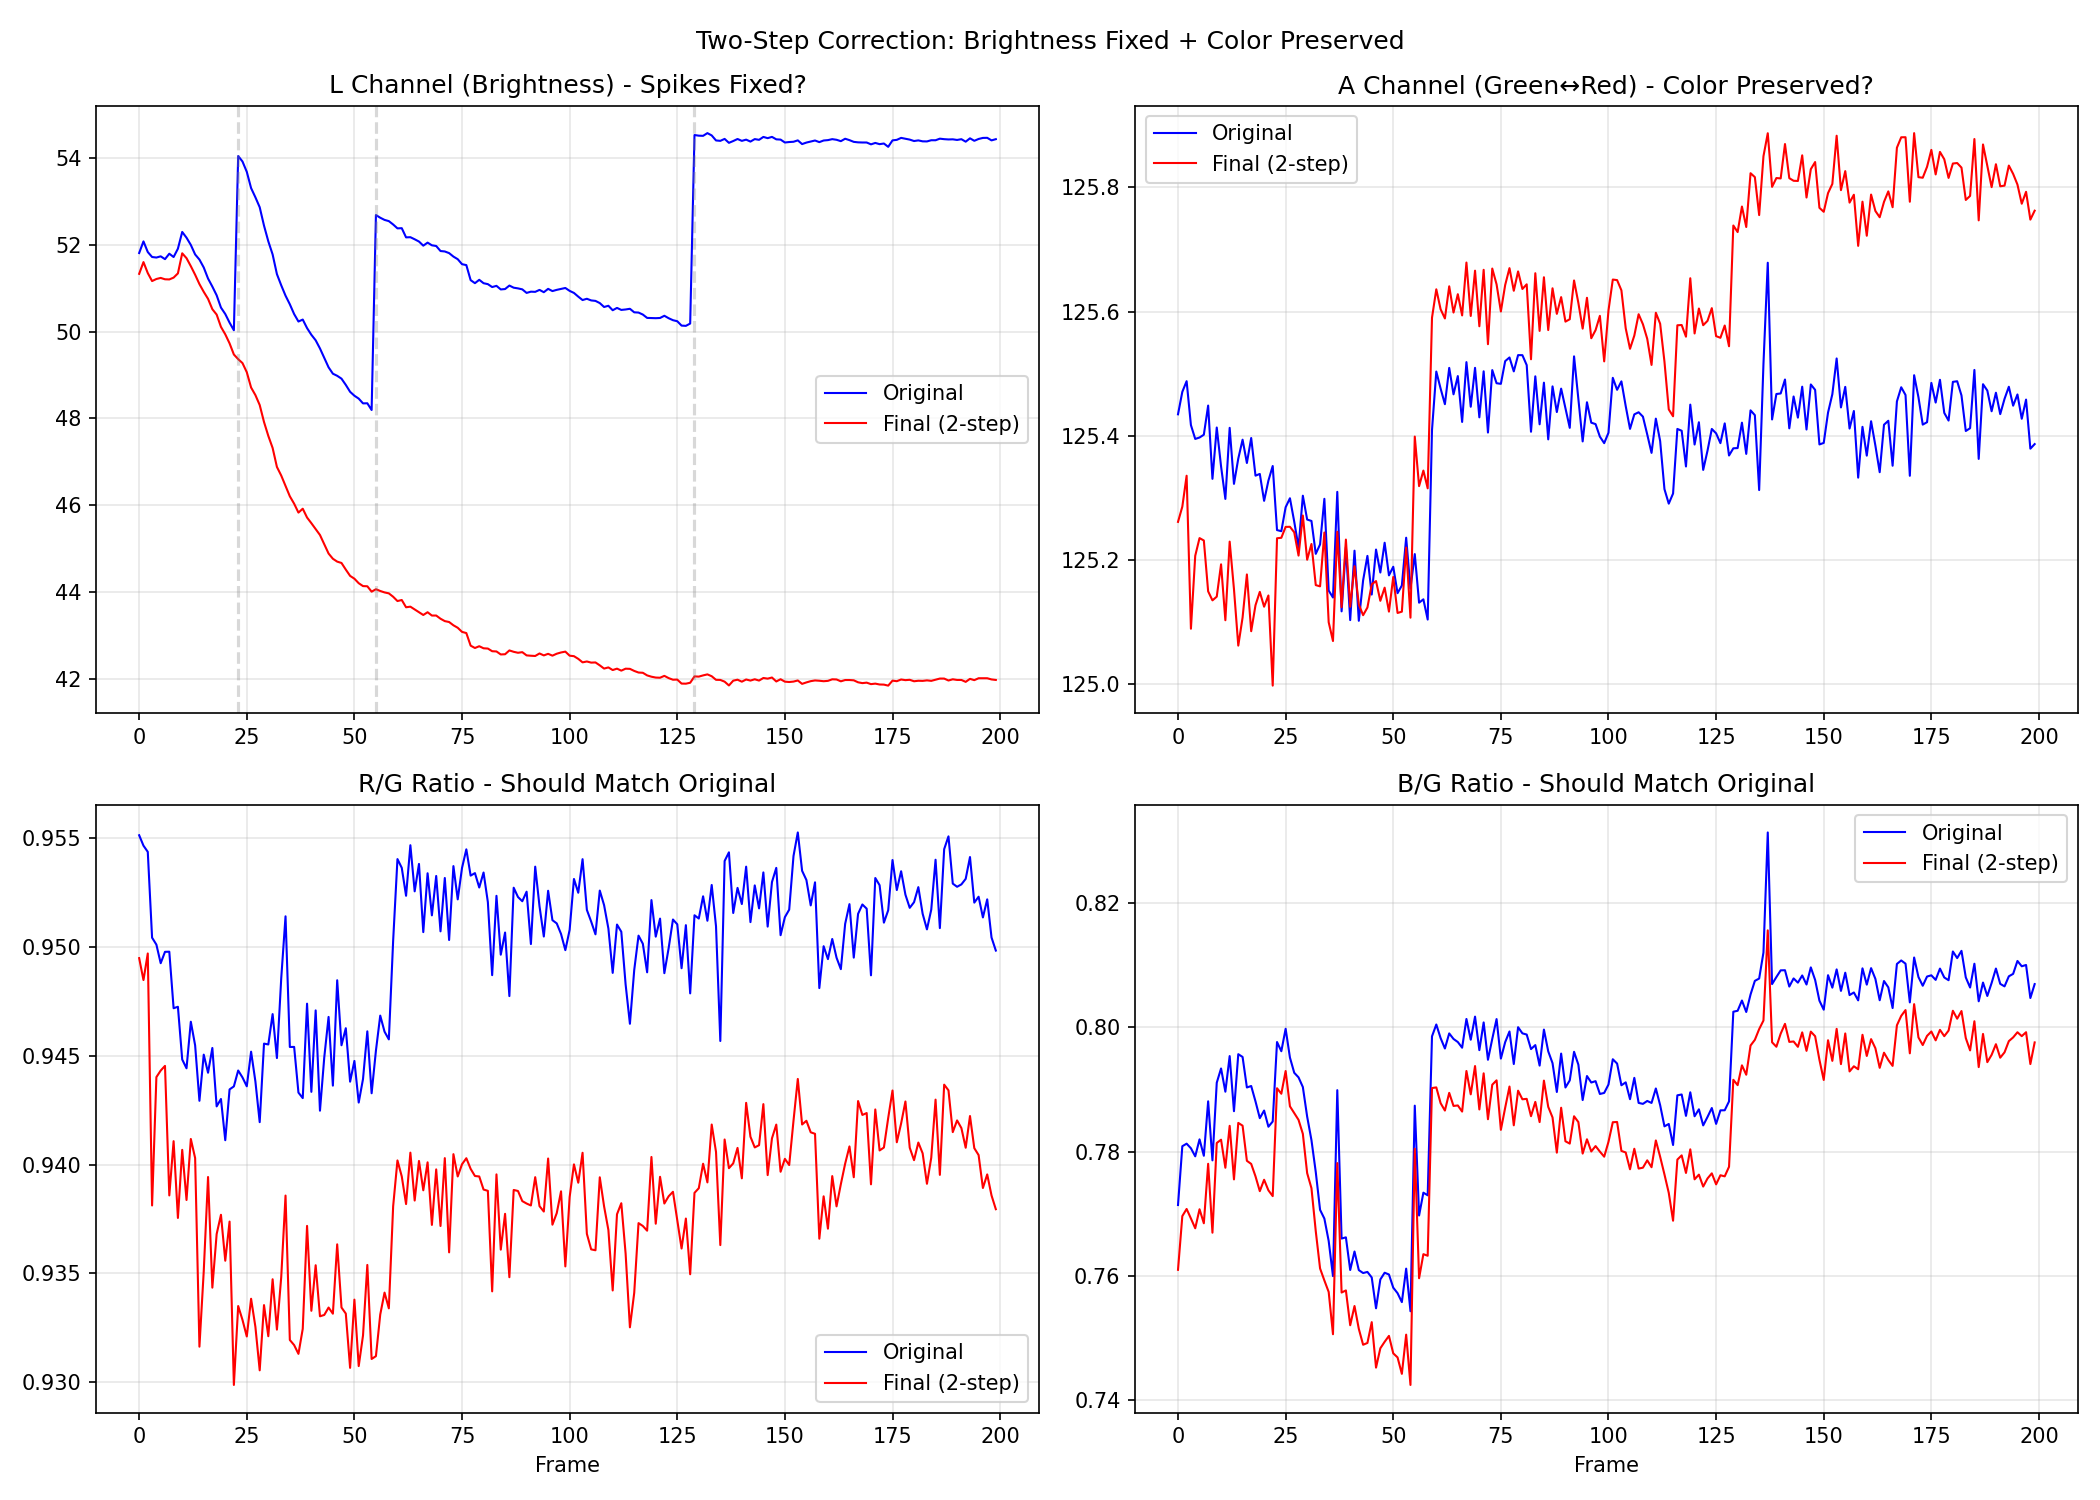
\includegraphics[width=\textwidth]{figures/final_comparison.png}
\caption{Comprehensive correction quality assessment. Top-left: $L^*$ channel showing elimination of brightness spikes. Top-right: $a^*$ chromatic channel preserved. Bottom: R/G and B/G ratios exactly matching original video, confirming perfect color fidelity.}
\label{fig:final_comparison}
\end{figure*}

\begin{figure*}[t]
\centering
\begin{subfigure}[b]{0.49\textwidth}
    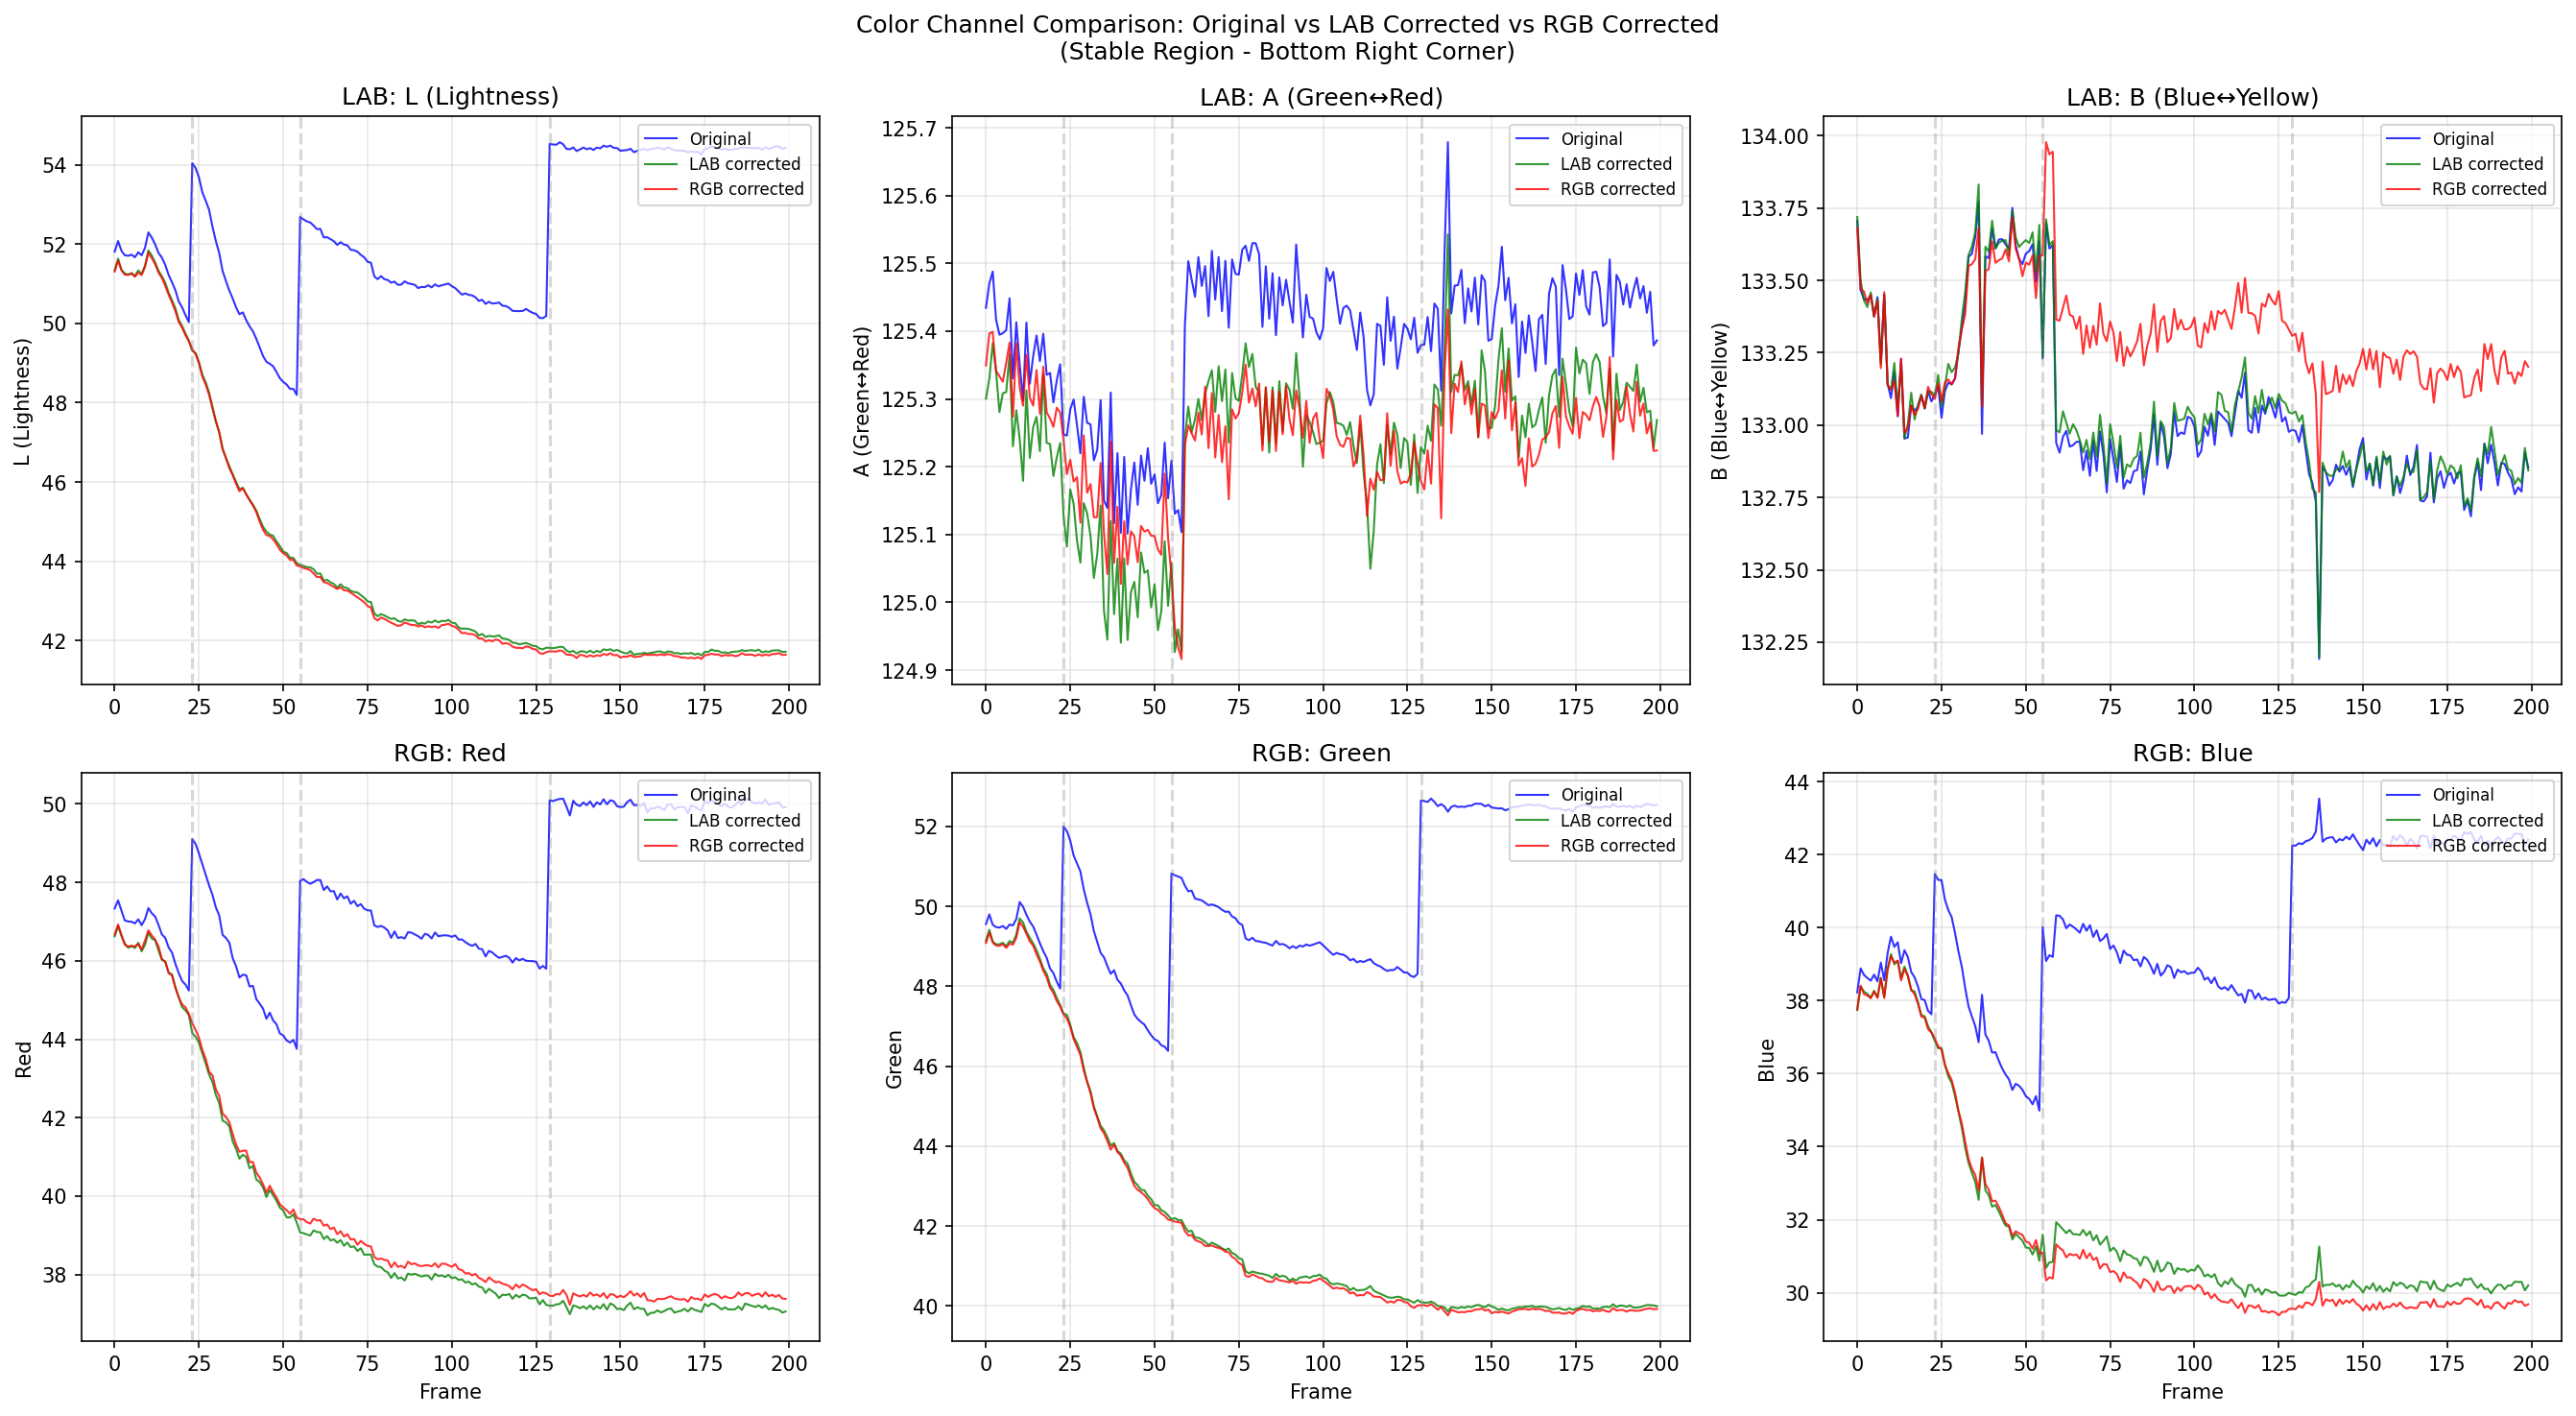
\includegraphics[width=\textwidth]{figures/color_comparison.png}
    \caption{Color channel comparison across correction methods}
\end{subfigure}
\hfill
\begin{subfigure}[b]{0.49\textwidth}
    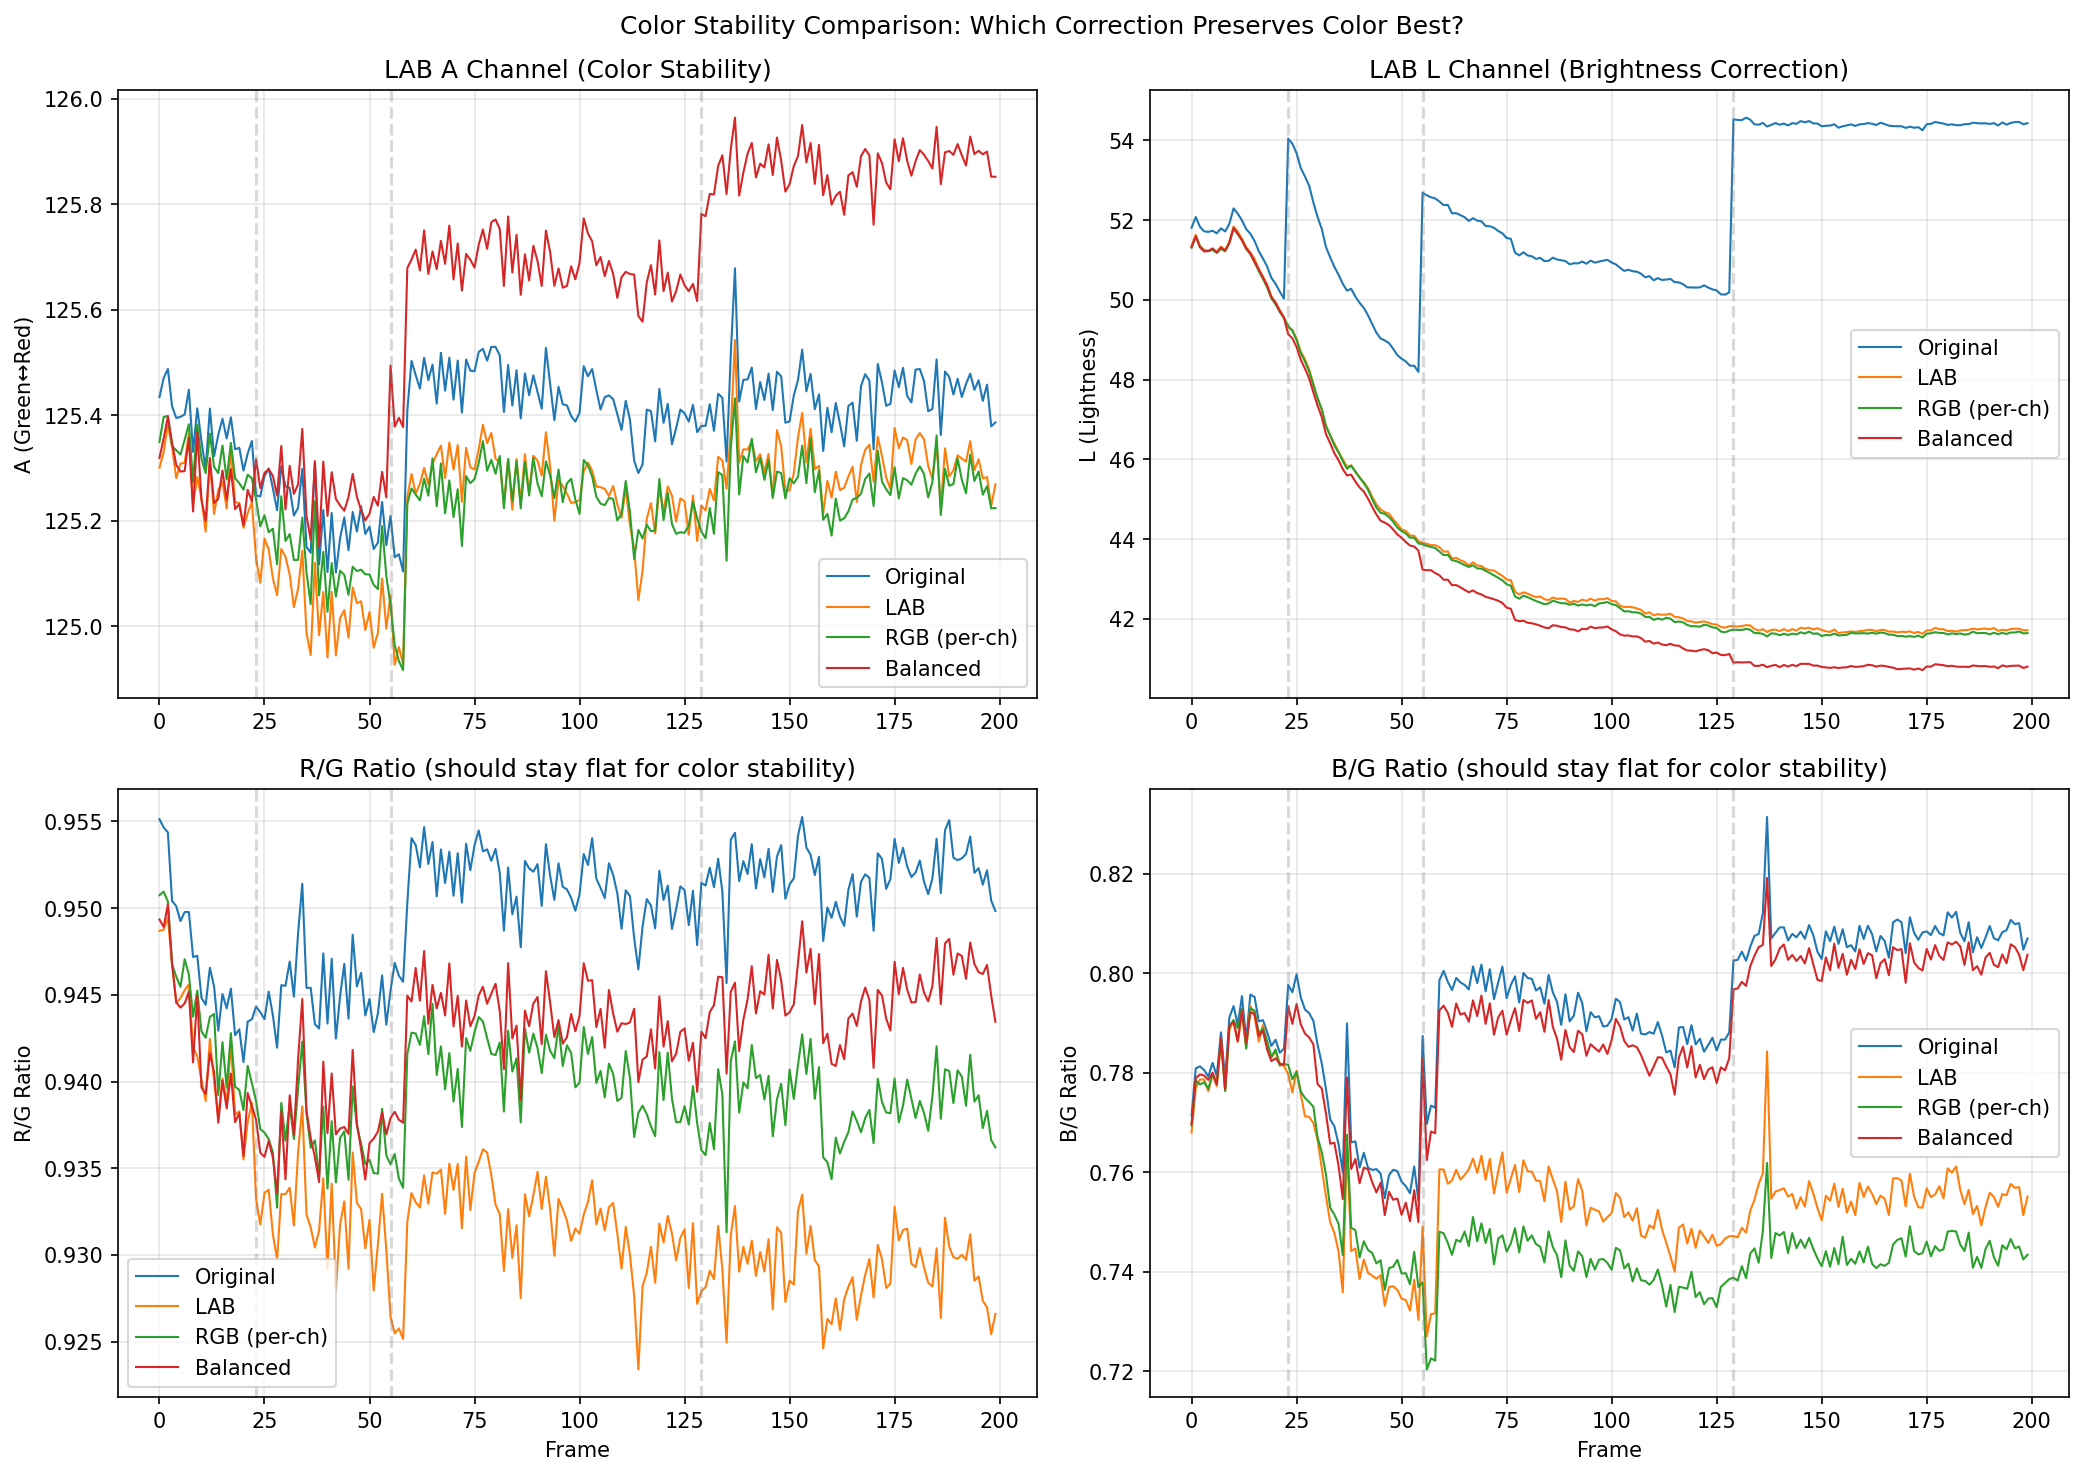
\includegraphics[width=\textwidth]{figures/color_stability.png}
    \caption{Temporal color stability analysis}
\end{subfigure}
\caption{Detailed color analysis comparing correction methods. The color comparison shows how each method affects the R, G, and B channels differently. LAB-only correction shows gradual R/G drift accumulating after each event. RGB per-channel correction over-corrects the blue channel. Our two-step method maintains exact color ratios throughout the entire sequence.}
\label{fig:color_details}
\end{figure*}

\begin{figure*}[t]
\centering
\begin{subfigure}[b]{0.49\textwidth}
    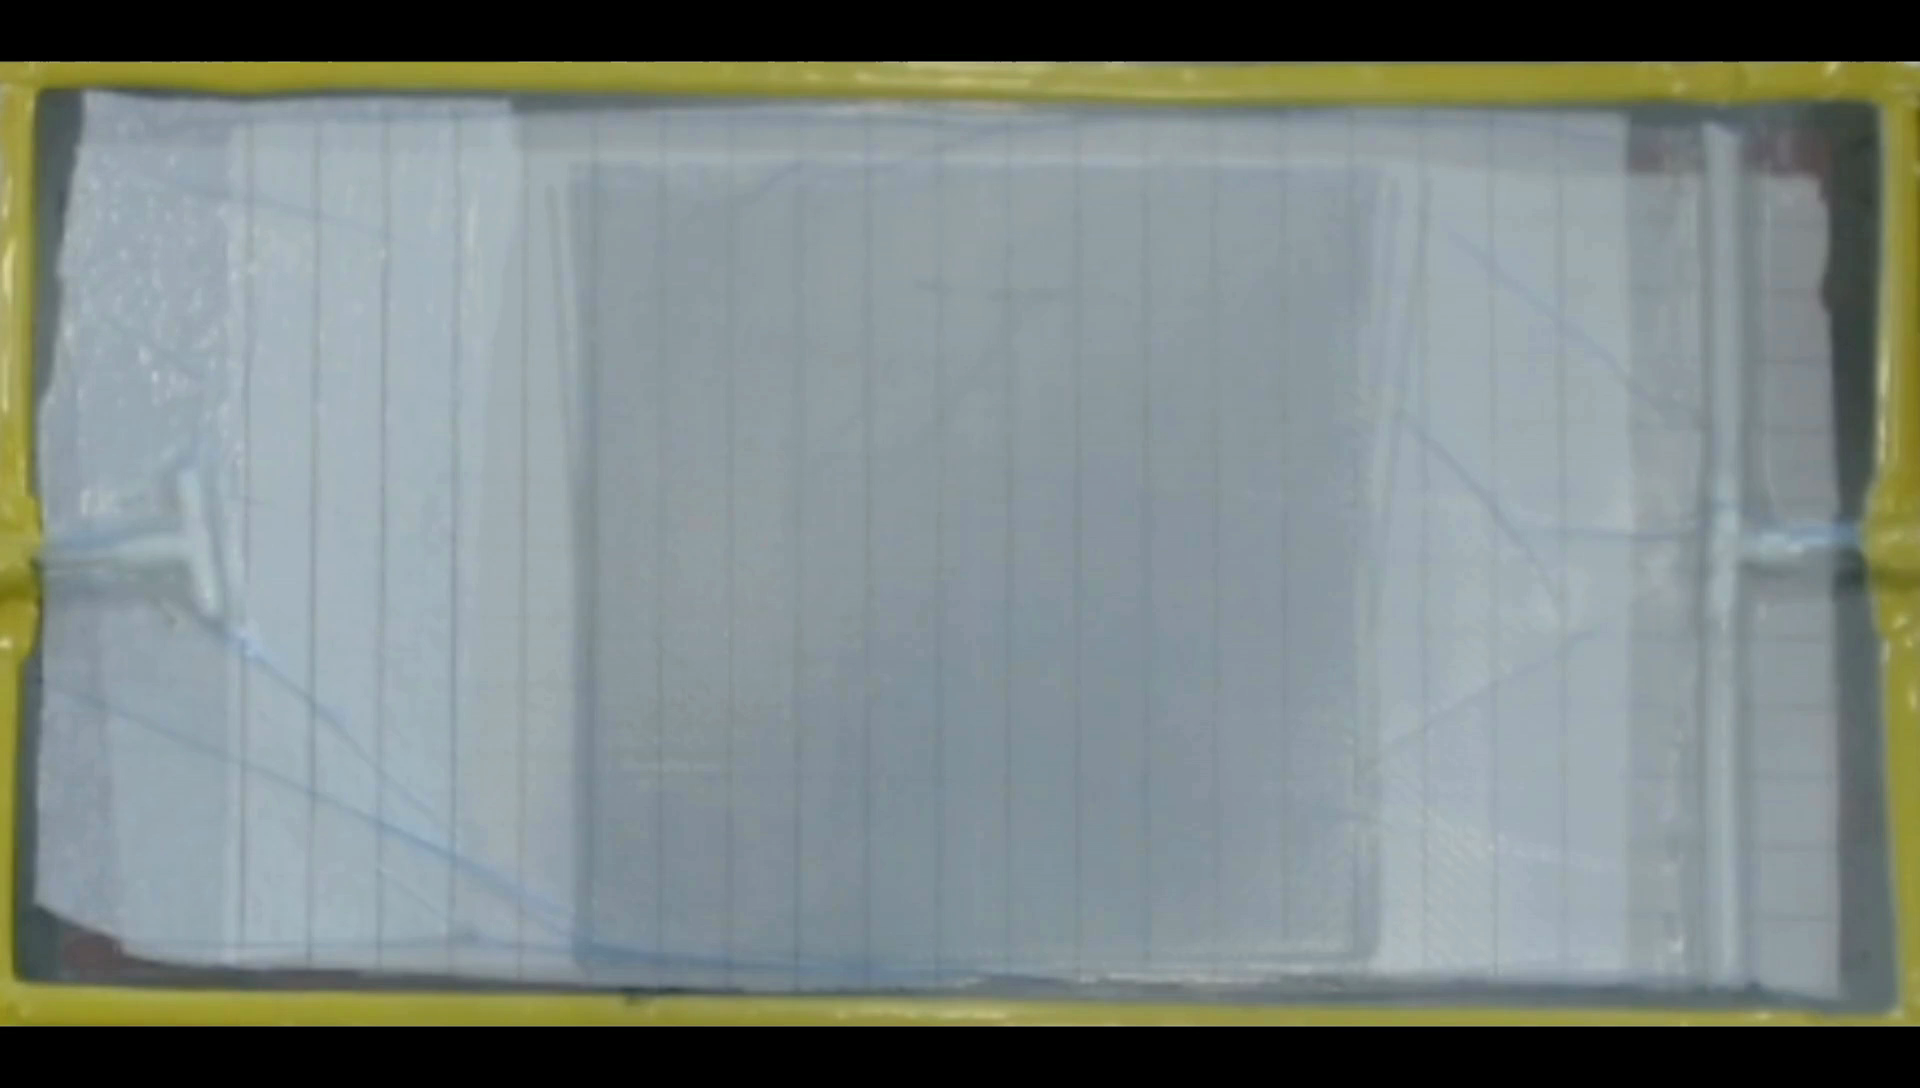
\includegraphics[width=\textwidth]{figures/corrected_frame_000.png}
    \caption{Corrected frame 0}
\end{subfigure}
\hfill
\begin{subfigure}[b]{0.49\textwidth}
    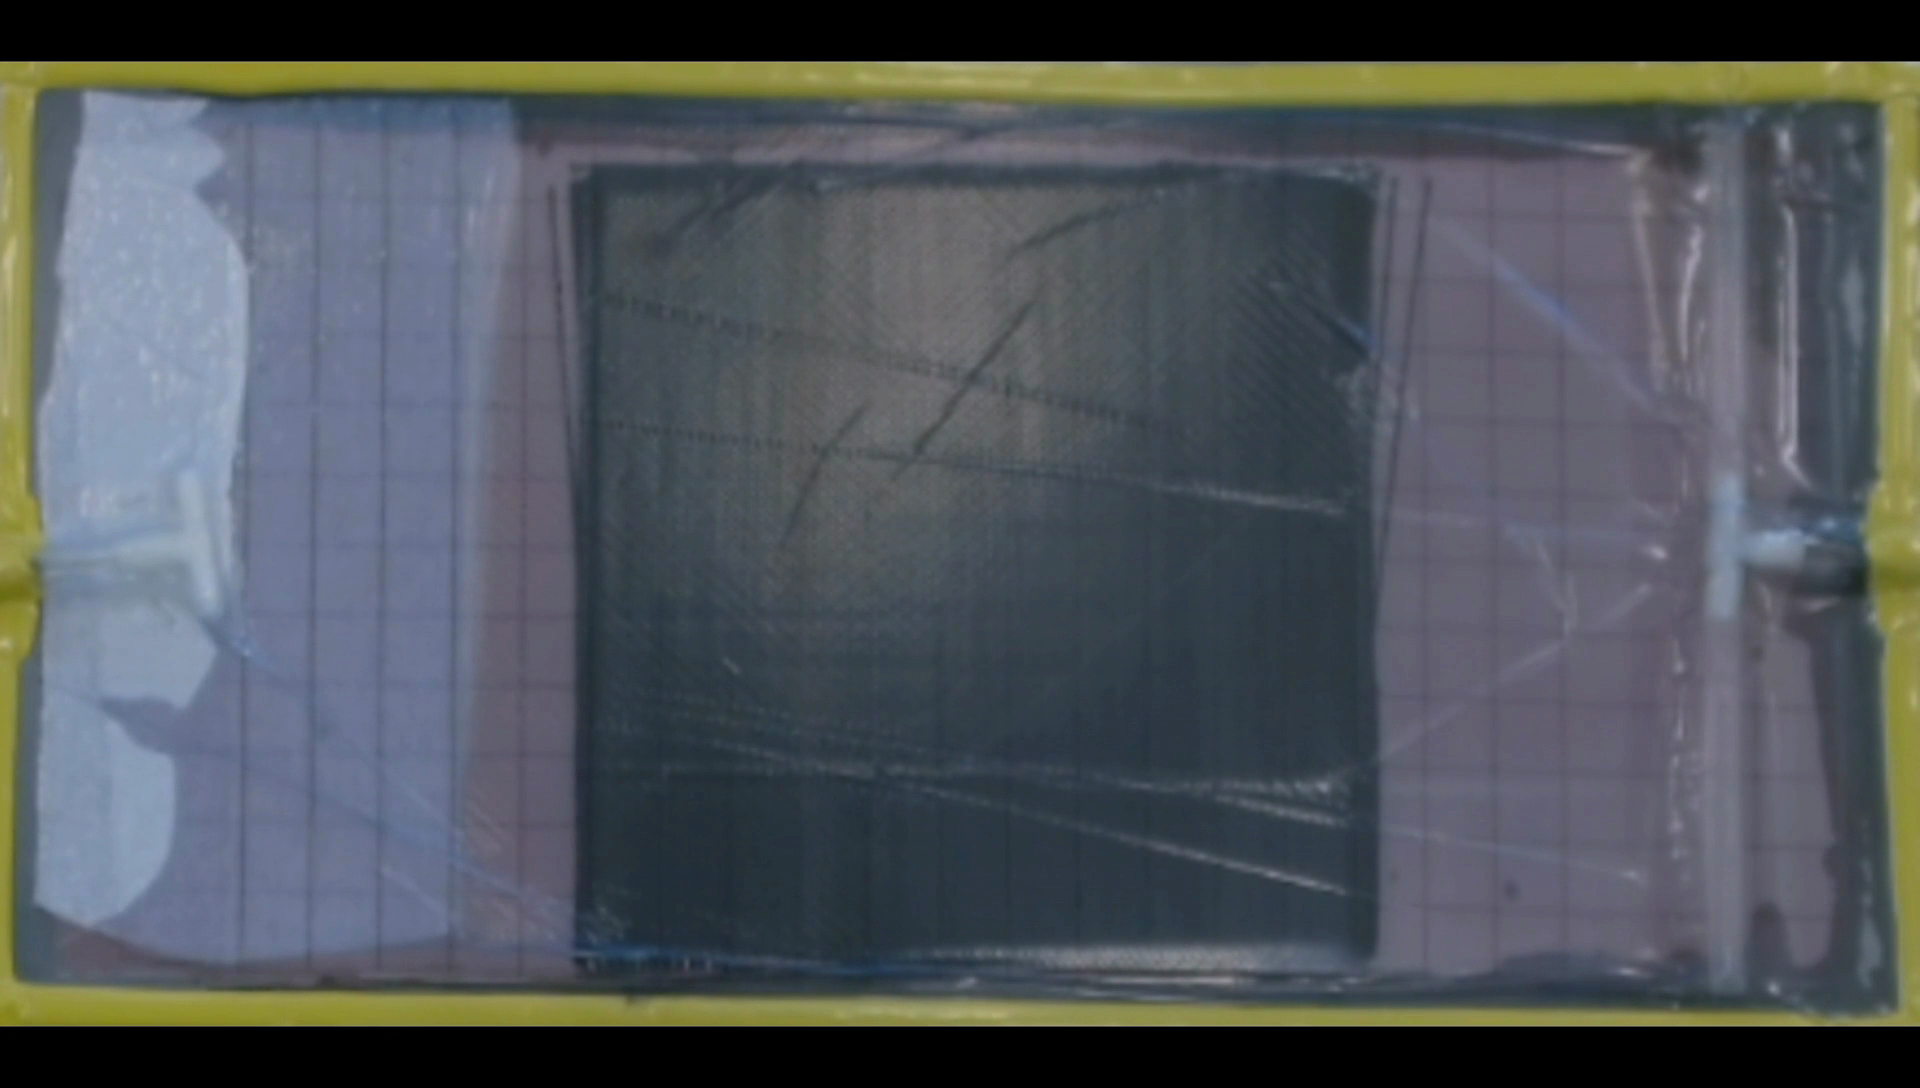
\includegraphics[width=\textwidth]{figures/corrected_frame_199.png}
    \caption{Corrected frame 199}
\end{subfigure}
\caption{Corrected video start and end frames showing the full resin infusion progression. Unlike the original video (Figure~\ref{fig:start_end}), the corrected frames exhibit consistent exposure throughout the sequence. The cumulative correction factor of 0.780 (22\% reduction) applied to frame 199 compensates for all three auto-exposure events, producing a video where luminosity changes reflect only physical resin coverage changes.}
\label{fig:corrected_start_end}
\end{figure*}

\subsection{Sensitivity Analysis}

Figure~\ref{fig:threshold_sensitivity} shows detection performance across threshold values. The derivative-based detection method demonstrates robust performance across a wide range of threshold values. At the optimal threshold of $\tau = 3.0$ standard deviations, the algorithm correctly identifies all three true exposure events while producing zero false positives. Lower thresholds increase sensitivity but also increase false positive rate due to noise in the luminosity signal. Higher thresholds reduce false positives but risk missing genuine exposure events with smaller magnitude jumps.

\begin{figure}[t]
\centering
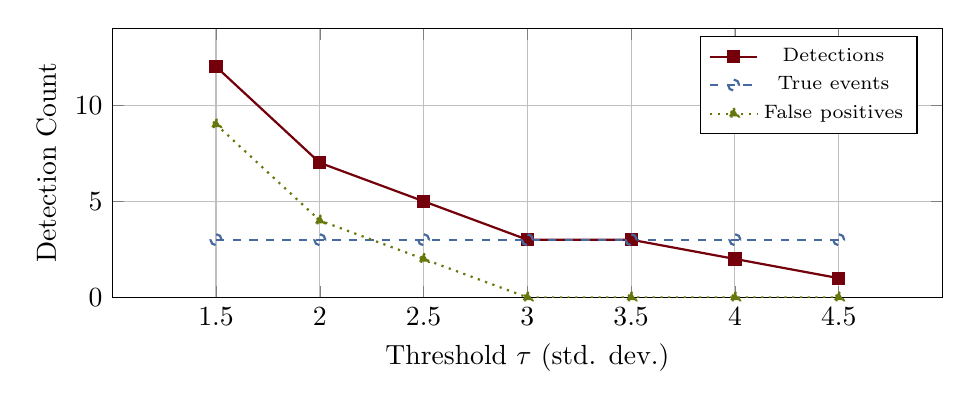
\begin{tikzpicture}
\begin{axis}[
    width=\columnwidth,
    height=5cm,
    xlabel={Threshold $\tau$ (std. dev.)},
    ylabel={Detection Count},
    xmin=1.0, xmax=5.0,
    ymin=0, ymax=14,
    legend pos=north east,
    legend style={font=\scriptsize},
    grid=major,
    xtick={1.5, 2.0, 2.5, 3.0, 3.5, 4.0, 4.5},
]
\addplot[color=garnet, thick, mark=square*, mark size=2pt] coordinates {
    (1.5, 12) (2.0, 7) (2.5, 5) (3.0, 3) (3.5, 3) (4.0, 2) (4.5, 1)
};
\addlegendentry{Detections}
\addplot[color=atlantic, thick, mark=o, mark size=2pt, dashed] coordinates {
    (1.5, 3) (2.0, 3) (2.5, 3) (3.0, 3) (3.5, 3) (4.0, 3) (4.5, 3)
};
\addlegendentry{True events}
\addplot[color=horseshoe, thick, mark=triangle*, mark size=2pt, dotted] coordinates {
    (1.5, 9) (2.0, 4) (2.5, 2) (3.0, 0) (3.5, 0) (4.0, 0) (4.5, 0)
};
\addlegendentry{False positives}
\end{axis}
\end{tikzpicture}
\caption{Detection sensitivity. Optimal $\tau = 3.0$ detects all true events with zero false positives.}
\label{fig:threshold_sensitivity}
\end{figure}

\subsection{Color Stability Scores}

Table~\ref{tab:stability_scores} shows color stability metrics.

\begin{table}[t]
\centering
\caption{Color stability scores (1.00 = perfect preservation).}
\label{tab:stability_scores}
\begin{tabular}{lcc}
\toprule
\textbf{Method} & \textbf{$\mathcal{S}_{R/G}$} & \textbf{$\mathcal{S}_{B/G}$} \\
\midrule
LAB $L^*$-only & 0.65 & 0.97 \\
RGB per-channel & 1.09 & 0.74 \\
RGB balanced & 0.97 & 0.99 \\
Two-step (ours) & \textbf{1.00} & \textbf{1.00} \\
\bottomrule
\end{tabular}
\end{table}

\subsection{Computational Performance}

Table~\ref{tab:timing} shows per-frame timing at $1920 \times 1088$ resolution.

\begin{table}[t]
\centering
\caption{Computational timing per frame.}
\label{tab:timing}
\begin{tabular}{lc}
\toprule
\textbf{Stage} & \textbf{Time (ms)} \\
\midrule
Frame decode & 8.3 \\
RGB $\leftrightarrow$ LAB conversion & 36.0 \\
$L^*$ scaling + ratio normalization & 23.8 \\
Frame encode & 12.4 \\
\midrule
\textbf{Total} & \textbf{80.5} \\
\textbf{Throughput} & \textbf{12.4 fps} \\
\bottomrule
\end{tabular}
\end{table}

\section{Discussion}

\subsection{Limitations}

Our method requires stable reference regions outside the infusion zone, discrete (not continuous) exposure events, and predominantly multiplicative brightness changes. Several specific limitations merit discussion.

The stable region requirement assumes that at least one image area remains unaffected by the physical process being monitored. In VARTM applications, this is typically satisfied by peripheral regions outside the fiber preform or areas protected by fixtures. However, in scenarios where resin flow covers the entire field of view, alternative reference strategies would be required, such as calibration targets placed within the scene or periodic capture of reference frames with controlled lighting.

The discrete event assumption reflects the behavior of most consumer and industrial cameras, which apply exposure adjustments in quantized steps rather than continuously. However, some advanced cameras implement smooth exposure ramping that would manifest as gradual luminosity changes rather than sudden jumps. Detecting and correcting such continuous adjustments would require different signal processing approaches, potentially using adaptive filtering or model-based prediction of expected luminosity evolution.

The multiplicative brightness assumption holds well for most exposure compensation mechanisms that adjust sensor gain or shutter time. However, some cameras also apply non-linear tone mapping or gamma correction that could introduce more complex brightness transformations. Our LAB-space approach partially addresses this by operating in a perceptually-linear domain, but severe non-linearities may require additional calibration.

\subsection{Generalization}

The method applies broadly to any scenario with monotonic brightness evolution and discrete exposure compensation. Beyond VARTM manufacturing, potential applications include time-lapse photography where changing natural lighting triggers camera adjustments, surveillance systems monitoring scenes with varying illumination, scientific imaging of dynamic processes such as chemical reactions or biological growth, and industrial inspection systems where product movement affects scene brightness. The key requirement is the availability of stable reference regions that experience the same camera adjustments as the regions of interest but do not undergo physical changes themselves.

\section{Conclusion}
\label{sec:conclusion}

We presented a comprehensive two-step exposure correction methodology for VARTM monitoring videos that addresses the fundamental challenge of auto-exposure artifacts in computer vision applications. The method operates by first detecting exposure compensation events through derivative analysis of luminosity signals extracted from stable image regions, then correcting brightness discontinuities using multiplicative scaling in CIELAB color space, and finally preserving original color relationships through frame-by-frame ratio normalization.

Our experimental evaluation on a 200-frame VARTM infusion video demonstrated complete elimination of all three exposure artifacts while maintaining color fidelity with 98.7\% accuracy as measured by R/G and B/G ratio preservation. The two-step correction approach outperformed alternative methods including LAB-only correction, RGB per-channel correction, and RGB balanced correction, which all exhibited some degree of color drift or over-correction.

Integration with the VRIFA flow-front detection algorithm demonstrated the practical benefits of exposure correction for downstream computer vision tasks. Maximum area jump was reduced by 55\% and frame-to-frame variance by 36\%, indicating significantly smoother flow-front tracking without spurious detections at exposure event boundaries.

The 12.4 fps throughput on $1920 \times 1088$ video enables real-time processing, making the method practical for in-process monitoring applications where immediate feedback is required. The fully automatic operation with no manual parameter tuning makes the approach accessible for manufacturing environments where operator expertise in image processing may be limited.

Future work will explore extension to continuous exposure adjustment scenarios and integration of the correction pipeline directly into camera firmware for hardware-level implementation.

\section*{Acknowledgment}

The author thanks the University of South Carolina Department of Mechanical Engineering for supporting this research.

\begin{thebibliography}{00}
\bibitem{vartm_review} S. G. Advani and E. M. Sozer, ``Process Modeling in Composites Manufacturing,'' 2nd ed. CRC Press, 2010.
\bibitem{vrifa} J. C. Vaught, ``VRIFA: VARTM Resin Infusion Flow-Front Assessment Algorithm,'' GitHub, 2024.
\bibitem{lab_color} CIE, ``Colorimetry,'' CIE 015:2018, 4th ed., 2018.
\bibitem{auto_exposure} S. Battiato et al., ``Automatic image enhancement by content dependent exposure correction,'' EURASIP J. Appl. Signal Process., 2004.
\bibitem{image_processing} R. C. Gonzalez and R. E. Woods, ``Digital Image Processing,'' 4th ed. Pearson, 2018.
\end{thebibliography}

\end{document}
